% pass biblatex options to the instance loaded by the class
\PassOptionsToPackage{backend=biber,style=authoryear,
                      sorting=none,      % bibliography in citation order
                      sortcites=false,
                      defernumbers=true}
{biblatex}
\PassOptionsToPackage{main=english}{babel}
\documentclass[master,intern,palatino]{rgseThesis}

\usepackage{booktabs}
\usepackage{setspace}
\usepackage[english]{babel}
\usepackage{csquotes}
\usepackage{graphicx}
\usepackage{xcolor}
\usepackage{amsmath}
\usepackage{amssymb}
\usepackage{caption}
\usepackage{subcaption}
\usepackage{float}
\usepackage{rotating}
\usepackage{longtable}
\usepackage{multirow}
\usepackage{makecell}
\usepackage{tabularx}
\usepackage{array}
\usepackage{enumitem}
\usepackage{listings}
\usepackage{hyperref}
\usepackage{fancyhdr}

\geometry{a4paper, margin=1in, includefoot, headheight=14.5pt, headsep=12pt}

% Running header: "N. Chapter Title" in top-right of every page.
\renewcommand{\chaptermark}[1]{\markboth{\thechapter.\ #1}{}}

% Title-page metadata
\author{Kazi Mostafa Shahriar\\[1ex] \normalsize Mat. Nr. 222100444 \\[1ex] \normalsize shahriar@uni-koblenz.de}

\title{Balancing Data Utility and Privacy in Medical Synthetic Data Generation: A Comparative Study of GAN-based and Large Language Model Approaches}

\supervisor{w}{Prof. Dr. Andreas Mauthe}
\supervisorInfo{Institut für Wirtschafts- und Verwaltungsinformatik, FG IT Security and Data Security}

\secondSupervisor{w}{Christopher Latz}
\secondSupervisorInfo{Institut für Wirtschafts- und Verwaltungsinformatik, FG IT Security and Data Security}

% Bibliography database
\addbibresource{literature.bib}

% TOC depth: 1 = sections, 2 = subsections, 3 = subsubsections
\setcounter{tocdepth}{3}
\setcounter{secnumdepth}{3}

\begin{document}

    \selectlanguage{english}
    \pagenumbering{roman}

    % Title page and declaration
    \maketitle

    % Abstract (German + English)
    % !TEX root = ../thesis.tex

% Abstract -- German (Zusammenfassung) + English

\begin{otherlanguage}{ngerman}
    \section*{Zusammenfassung}

    Die Freigabe medizinischer Daten f\"ur die Forschung wird durch
    Datenschutzregelungen wie HIPAA und DSGVO eingeschr\"ankt, w\"ahrend sich
    klassische Anonymisierungsverfahren gegen\"uber Verkn\"upfungs- und
    Re-Identifikationsangriffen wiederholt als unzureichend erwiesen haben.
    Die Erzeugung synthetischer Daten bietet eine Alternative, doch der
    Zielkonflikt zwischen Nutzbarkeit und Privatsph\"are ist \"uber
    grundlegend verschiedene generative Paradigmen hinweg bislang nur
    unzureichend charakterisiert. Diese Arbeit pr\"asentiert einen
    einheitlichen empirischen Vergleich von f\"unf Generatoren auf dem
    Datensatz \emph{Diabetes 130-US Hospitals}, der die GAN- und die
    LLM-Familie jeweils mit und ohne formale Differential Privacy abdeckt:
    HealthGAN, PATE-GAN, Pythia-70M-LoRA, Pythia-1B-LoRA und
    Pythia-1B-DP-LoRA. Jeder Generator wird anhand skalarer Metriken entlang
    zweier S\"aulen bewertet: \emph{Utility}, die statistische \"Ahnlichkeit
    zu den realen Daten mit der pr\"adiktiven Leistung nachgelagerter, auf
    synthetischen Datens\"atzen trainierter Modelle verbindet, und
    \emph{Privacy}, die instanzbasierte Distanzma{\ss}e sowie Membership- und
    Attribute-Inference-Risiken umfasst.

    Keine der beiden Familien dominiert durchg\"angig. Ohne formale Garantie
    bleibt die Wahl ein echter Zielkonflikt: HealthGAN erreicht die beste
    marginale Fidelit\"at und als einziger nutzbarer Generator ein
    N\"achste-Nachbarn-Distanzverh\"altnis an der Einheitsreferenz. Die
    Sprachmodelle erzielen die h\"ochste pr\"adiktive Utility, wobei
    Pythia-1B der realen Referenz am n\"achsten kommt (AUC $0.682$
    gegen\"uber $0.701$). Unter einem angeglichenen Budget
    ($\varepsilon = 5.0$) verschiebt sich die Balance zugunsten der
    LLM-Familie: Pythia-1B-DP bleibt f\"ur einen R\"uckgang von etwa $0.10$
    im TSTR-AUC-ROC nutzbar, beseitigt zugleich das beim nicht-privaten
    Gegenst\"uck beobachtete Attribute-Inference-Leck und senkt die
    Outlier-Linkability auf null. Das hier evaluierte differentiell private
    GAN bricht dagegen auf beiden Utility-Zweigen ein und erzielt lediglich
    die scheinbare Privatheit einer von der realen Datenverteilung
    entfernten Ausgabe. Die Kosten der Differential Privacy sind somit stark
    familienabh\"angig. Die Arbeit liefert eine reproduzierbare
    Evaluationspipeline, einen direkten Benchmark entlang der GAN-LLM- und
    der DP-nicht-DP-Achse sowie quantitative Evidenz zu den Grenzkosten
    formaler Differential Privacy innerhalb jeder Generatorfamilie.
\end{otherlanguage}
\cleardoublepage

\begin{otherlanguage}{english}
    \section*{Abstract}

    Privacy regulations such as Health Insurance Portability and Accountability Act 
    (HIPAA) and General Data Protection Regulation (GDPR) provide the governance 
    framework within which medical data can be shared and reused responsibly 
    for research., while classical anonymisation has
    proven insufficient under linkage and re-identification attacks. Synthetic
    data generation offers an alternative, yet the trade-off between utility and
    privacy remains poorly characterised across fundamentally different
    generative paradigms. This thesis presents a unified empirical comparison of
    five generators on the \emph{Diabetes 130-US Hospitals} dataset, spanning
    the Generative Adversarial Network (GAN) and Large Language Model (LLM) 
    families both with and without formal differential privacy:
    HealthGAN, PATE-GAN, Pythia-70M-LoRA, Pythia-1B-LoRA, and Pythia-1B-DP-LoRA.
    Every generator is assessed with single-number metrics across two pillars:
    \emph{utility}, combining statistical similarity to the real data with the
    downstream predictive performance of models trained on the synthetic
    records, and \emph{privacy}, covering instance-level distance and
    membership- and attribute-inference risk.

    Without a formal guarantee the choice is a
    genuine trade-off: HealthGAN attains the best marginal fidelity and the only
    distance ratio at the nearest-neighbour unity reference. The language models
    reach the highest predictive utility, with Pythia-1B closest to the
    real-data ceiling (AUC $0.682$ against $0.701$). Under a matched
    $(\varepsilon = 5.0)$ budget the balance tips toward the LLM family:
    Pythia-1B-DP stays usable for roughly a $0.10$ drop in TSTR AUC-ROC while
    removing its non-private counterpart's observed attribute-inference leak
    and driving outlier linkability to zero. The differentially private GAN
    evaluated here, by contrast, collapses on both utility branches and earns
    only the apparent privacy of off-manifold output. The cost of differential privacy is thus
    strongly family-dependent. The thesis contributes a reproducible evaluation
    pipeline, a head-to-head benchmark spanning the GAN-LLM and DP-non-DP axes,
    and quantitative evidence on the marginal cost of formal differential
    privacy within each generative family.
\end{otherlanguage}
\cleardoublepage


    \tableofcontents
    \cleardoublepage

    \listoffigures
    \cleardoublepage

    \listoftables
    \cleardoublepage

    \pagenumbering{arabic}

    % Activate running header for main matter: chapter on top-right, page
    % number bottom-centre. Chapter-opening pages stay plain by default.
    \pagestyle{fancy}
    \fancyhf{}
    \fancyhead[R]{\nouppercase{\leftmark}}
    \fancyfoot[C]{\thepage}
    \renewcommand{\headrulewidth}{0.4pt}
    \fancypagestyle{plain}{%
        \fancyhf{}%
        \fancyfoot[C]{\thepage}%
        \renewcommand{\headrulewidth}{0pt}%
    }

    % --- Main chapters ---
    % !TEX root = ../thesis.tex

\chapter{Introduction}
\label{ch:introduction}

\section{Background and Motivation}
\label{sec:intro:motivation}

% Migrated and lightly edited from proposal §1 (Introduction) + §2 (Motivation).
The sustained growth of digital health records, together with rapid advances
in artificial intelligence (AI), offers significant potential to transform
healthcare delivery. At the same time, robust regulatory frameworks such as the
General Data Protection Regulation (GDPR) and the Health Insurance Portability
and Accountability Act (HIPAA) play a crucial role in safeguarding patient
confidentiality and ensuring responsible data use. These protections are
essential for maintaining public trust in digital health systems. They also
require researchers to explore innovative methods that enable data-driven
innovation while upholding proper privacy standards. Conventional anonymisation
methods have repeatedly proven insufficient to guarantee privacy in
high-dimensional health data, as re-identification and linkage attacks remain
viable~\cite{Murtaza2023,stadler2022synthetic}.

Synthetic data generation (SDG) has emerged as a promising alternative,
enabling the creation of artificial datasets that retain the statistical
properties of the original while mitigating privacy risks. Among the most
prominent approaches are \emph{Generative Adversarial Networks} (GANs) and
\emph{Large Language Models} (LLMs). GANs have demonstrated success in
structured medical records~\cite{Choi2017MedGAN,Xu2019CTGAN},
and imaging data, while transformer-based LLMs
offer advantages in modelling heterogeneous and unstructured
records~\cite{Miletic2024}. GANs work by training
two neural networks: a generator that creates synthetic samples and a
discriminator that tries to distinguish them from real data until the
generator learns to produce highly realistic outputs. LLMs
operate using transformer architectures that leverage self-attention to learn
long-range patterns in sequences, allowing them to generate coherent text or
structured records. While GANs focus on matching data distributions through
adversarial learning, LLMs generate data by predicting the next most probable
token based on context.

The need for privacy-preserving data generation in healthcare is not only a
technical challenge but a foundational concern of medical research. The
scarcity of openly accessible, high-quality clinical data constrains
innovation in diagnosis, treatment planning, and epidemiological modelling.
Regulatory restrictions and ethical imperatives make direct sharing of
identifiable records infeasible. Synthetic data presents a pathway to alleviate
this bottleneck by allowing the distribution of data without direct disclosure
of personal identifiers, thus accelerating AI model development and
validation.

\section{Problem Statement: The Utility--Privacy Tension}
\label{sec:intro:problem}

The adoption of synthetic data in healthcare depends on two interdependent
requirements: utility and privacy. Synthetic data is valuable only if it remains
analytically useful, and defensible only if it reduces the risk of exposing
information about real patients. The core problem is therefore not to optimise
either criterion in isolation, but to understand the trade-off between them.

\begin{enumerate}\itemsep0.25em
  \item \textbf{Utility:} the dataset must preserve the statistical,
        structural, and predictive characteristics needed for downstream
        analysis, including marginal feature distributions, variable
        dependencies, target class balance, and model generalisation to real
        held-out data.
  \item \textbf{Privacy:} the dataset must provide resistance to adversarial
        attacks, such as membership inference, attribute disclosure, and
        record-level linkage, especially when rare diagnoses, unusual treatment
        patterns, or repeated encounters make patients identifiable even after
        direct identifiers have been removed.
\end{enumerate}
While GANs and LLMs each offer unique strengths, there is limited comparative
work evaluating their effectiveness under a unified privacy--utility framework,
particularly for heterogeneous healthcare datasets.

\section{Research Questions}
\label{sec:intro:rqs}

This thesis addresses three research questions.

\paragraph{RQ1:}
\label{rq:rq1} Which methods and metrics are suitable for evaluating the
utility (statistical resemblance and predictive performance) and privacy risk
of synthetic tabular medical data, and what distinct dimension of data
characteristics does each capture?

\paragraph{RQ2:}
\label{rq:rq2} How do GAN-based and LLM-based synthesisers compare on the
privacy--utility trade-off when applied to tabular medical data, and which
achieves a more effective balance?

\paragraph{RQ3:}
\label{rq:rq3} At a matched privacy budget ($\varepsilon = 5.0$), how does
enforcing differential privacy using mechanisms appropriate to each family
affect utility, and how do the resulting privacy--utility profiles differ
between GAN-based (PATE-GAN vs.\ HealthGAN) and LLM-based (Pythia-1B-DP vs.\
Pythia-1B) synthesisers of tabular medical data?

\section{Contributions}
\label{sec:intro:contributions}

This thesis makes four main contributions to the evaluation of
privacy-preserving synthetic tabular health data.

First, it develops a reproducible evaluation pipeline for synthetic medical
tabular data. The pipeline is organised around two complementary dimensions:
\emph{utility}, comprising both statistical similarity to the real data and the
predictive performance of downstream models, and \emph{privacy}, covering
proximity-based memorisation indicators, membership-inference risk,
attribute-inference risk, and outlier linkability.

Second, it provides a head-to-head empirical comparison of five generators on
the \emph{Diabetes 130-US Hospitals} dataset~\cite{diabetes_db}: HealthGAN
(WGAN-GP)~\cite{healthgan}, PATE-GAN
($(\varepsilon,\delta)$-DP)~\cite{pategan}, Pythia-70M-LoRA and
Pythia-1B-LoRA~\cite{Biderman2023Pythia,Hu2022LoRA,Miletic2024}, and
Pythia-1B-DP-LoRA using DP-SGD via
Opacus~\cite{Yousefpour2021Opacus,Abadi2016DPSGD}.

Third, it quantifies the marginal cost of formal differential privacy within
both model families: non-DP HealthGAN versus PATE-GAN at $\varepsilon=5.0$ in
the GAN setting, and non-DP Pythia-1B versus Pythia-1B-DP at
$\varepsilon=5.0$ in the LLM setting. The inclusion of the non-DP Pythia-1B
scale anchor and the Pythia-1B-DP variant constitutes a scope extension beyond
the originally submitted proposal, motivated by the finding that DP-SGD applied
to Pythia-70M does not converge usefully at this privacy budget
(\S\ref{sec:results:rq3:pythia-70m-failure}).

Fourth, it derives practical recommendations for medical data stewards. These
recommendations identify when a non-DP GAN may be sufficient, which
differentially private mechanism is preferable when a formal guarantee is
required, and under which privacy-budget and governance constraints LLM-based
synthesis is competitive.

\section{Thesis Outline}
\label{sec:intro:outline}

The remainder of this thesis is structured as follows.
\textbf{Chapter~\ref{ch:background}} surveys the background and related work
on tabular synthetic data generation, GAN- and LLM-based approaches,
differential privacy, and existing evaluation frameworks.
\textbf{Chapter~\ref{ch:methodology}} consolidates the experimental
methodology of the thesis. Section~\ref{sec:method:data} describes the
\emph{Diabetes 130-US Hospitals} benchmark and the feature-engineering
pipeline used to prepare it for synthesis.
Section~\ref{sec:method:generators} details the five generators compared in
this work: HealthGAN, PATE-GAN, Pythia-70M-LoRA, Pythia-1B-LoRA, and
Pythia-1B-DP-LoRA, including architectures, training protocols, and the
differentially private mechanisms employed. Section~\ref{sec:method:evaluation} defines the unified
two-pillar evaluation framework: utility (statistical similarity and
predictive performance) and privacy.
\textbf{Chapter~\ref{ch:results}} reports the empirical findings, structured
around the three research questions.
\textbf{Chapter~\ref{ch:discussion}} interprets the results, discusses
strengths and weaknesses of each generator, and acknowledges threats to
validity. Finally, \textbf{Chapter~\ref{ch:conclusion}} summarises the
contributions, returns directly to RQ1--RQ3, and outlines avenues for future
work.

\cleardoublepage

    % !TEX root = ../thesis.tex

\chapter{Background and Related Work}
\label{ch:background}

% This chapter migrates and expands proposal §4 (Literature Review) and adds
% the technical background sections needed to support Chapters 4 and 5.

\section{Medical Tabular Data and Privacy Regulations}
\label{sec:bg:regulations}

Classical anonymisation methods like generalisation, suppression, distortion,
swapping, masking, and the $k$-anonymity / $\ell$-diversity / $t$-closeness
lineage struggle to preserve utility on high-dimensional EHR data and have
repeatedly been shown vulnerable to linkage and inference
attacks~\cite{anonymization,Murtaza2023}. Synthetic data sidesteps direct
release of real records but does not automatically resolve the trade-off:
\textcite{stadler2022synthetic} show that non-DP synthetic data still leaks
information about outliers, motivating the formal privacy machinery
(§\ref{sec:bg:dp}) used by the DP generators in this thesis. 
\section{Synthetic Data Generation: A Taxonomy}
\label{sec:bg:taxonomy}

Synthetic tabular data generators fall broadly into statistical models (copulas,
Bayesian networks, sequential trees), deep generative models (GAN- and
VAE-based), and language-model-based approaches that treat rows as
text~\cite{hernandez2022synthetic,Murtaza2023}. Alongside these data-driven
families, \textcite{Murtaza2023} also describe a knowledge-driven approach that
builds generators from hand-curated expert rules, and a hybrid approach that
blends the two; both remain labour-intensive and predominantly knowledge-driven,
and therefore fall outside the fully data-driven scope of this thesis. Each
family admits a differentially-private variant, yielding the GAN/LLM $\times$ DP/non-DP axes
along which the five generators evaluated in this thesis are positioned. The
remainder of the chapter develops the two families used here
(§\ref{sec:bg:gan}, §\ref{sec:bg:llm}) and the DP machinery they rely on
(§\ref{sec:bg:dp}). Unlike image 
or text data, which consist of uniform basic units amenable to a single modelling 
paradigm, tabular data combines categorical and numerical columns with heterogeneous 
statistical properties which is a challenge that no single generative family solves cleanly, 
and that drives the proliferation of distinct approaches surveyed in \cite{shi2025comprehensive}.
 Within each family, known failure modes (training instability and mode collapse in GANs,
 a tendency toward over-averaged outputs in VAEs, and hallucination in LLMs) have
 motivated successive specialisations, including the diffusion-model and fine-tuned-LLM
 branches that occupy the DP/non-DP axes evaluated in this thesis.


\section{GAN-based Approaches for Tabular Data}
\label{sec:bg:gan}

Generative adversarial networks constitute the dominant deep generative
paradigm for tabular synthesis, yet inherit the training instability and
mode-collapse pathologies first documented in the image
domain~\cite{shi2025comprehensive}. The remainder of this section reviews
the architectural progression from the original minimax formulation through
the Wasserstein and gradient-penalty refinements that stabilise adversarial
training (§\ref{sec:bg:gan:foundations}), and subsequently examines the two
healthcare-oriented variants situated on the DP and non-DP axes evaluated
in this thesis: HealthGAN (§\ref{sec:bg:gan:health}) and
PATE-GAN (§\ref{sec:bg:gan:pategan}).


\subsection{Foundations: GAN, WGAN, WGAN-GP}
\label{sec:bg:gan:foundations}

Generative adversarial networks formulate data generation as a
minimax game between a generator $G$, which maps noise samples into
the data space, and a discriminator $D$, which estimates the
probability that a given sample originates from the data distribution
rather than from $G$~\cite{Goodfellow2014GAN}:
\begin{equation}
\label{eq:gan-minimax}
\min_{G} \max_{D}\; V(D, G) =
\mathbb{E}_{x \sim p_{\text{data}}}\!\left[\log D(x)\right]
+ \mathbb{E}_{z \sim p_z}\!\left[\log\bigl(1 - D(G(z))\bigr)\right].
\end{equation}
The global optimum is attained when the generator distribution
matches the data distribution and the discriminator is everywhere
indifferent. In practice, however, optimisation of this objective is
fragile: the discriminator can saturate and starve the generator of
gradient signal, the value function offers no monotonic indicator of
convergence, and the generator is prone to mode collapse, in which
it concentrates mass on a narrow subset of plausible samples.

These pathologies have been attributed to the implicit
Jensen--Shannon divergence underlying the original objective, which
is discontinuous in the generator's parameters whenever the model
and data distributions have disjoint or near-disjoint
supports~\cite{Arjovsky2017WGAN}. Replacing it with the Wasserstein-1
distance restores continuity throughout training and yields a
gradient that remains informative even in this regime. Via the
Kantorovich--Rubinstein duality, the Wasserstein-1 distance admits
the variational form
\begin{equation}
\label{eq:wasserstein-dual}
W(p_{\text{data}}, p_g)
= \sup_{\|f\|_{L} \leq 1}\;
\mathbb{E}_{x \sim p_{\text{data}}}\!\left[f(x)\right]
- \mathbb{E}_{x \sim p_g}\!\left[f(x)\right],
\end{equation}
so that the discriminator is replaced by a 1-Lipschitz \emph{critic}
whose scalar output approximates this supremum. The Lipschitz
constraint is enforced in the original Wasserstein GAN by clipping
the critic's weights to a fixed interval, a modification that
produces markedly stabler training and a loss that correlates with
sample quality.

Weight clipping, however, was subsequently shown to be the source of
its own pathologies, chief among them a sharp loss of critic
capacity and gradient norms that either explode or vanish depending
on the clipping threshold~\cite{Gulrajani2017WGANGP}. The improved
formulation replaces clipping with a soft penalty on the critic's
input-gradient norm,
\begin{equation}
\label{eq:wgan-gp}
\mathcal{L}
= \mathbb{E}_{\tilde{x} \sim p_g}\!\left[D(\tilde{x})\right]
- \mathbb{E}_{x \sim p_{\text{data}}}\!\left[D(x)\right]
+ \lambda \,
\mathbb{E}_{\hat{x}}\!\left[
\bigl(\|\nabla_{\hat{x}} D(\hat{x})\|_{2} - 1\bigr)^{2}
\right],
\end{equation}
where $\hat{x}$ is sampled uniformly along straight lines between
paired real and generated samples. The penalty encourages the
critic to satisfy the Lipschitz condition with unit norm along the
region of the input space where the two distributions are being
compared, rather than uniformly across its parameters. This
Wasserstein-with-gradient-penalty formulation is the backbone on
which HealthGAN (§4.2) and its differentially-private extension
(§2.5) are built.

\subsection{Healthcare-specific Variants: HealthGAN}
\label{sec:bg:gan:health}

HealthGAN was introduced as a response to the limitations of medGAN, which
could only generate binary diagnosis codes and often produced unrealistic
distributions, making it unsuitable for mixed-type EHR
data~\cite{healthgan,yale2020synthesizing,bhanot2022investigating}. To address
these shortcomings, the model combines medGAN's design with the WGAN-GP
framework, leveraging the Wasserstein distance and a tailored data
transformation pipeline to support continuous and categorical variables
commonly found in datasets such as MIMIC-III~\cite{healthgan}. Its architecture
employs large batch sizes to ensure that outliers and rare clinical values are
reliably captured, and incorporates a bottleneck to reduce memorisation and
maintain a compact model footprint, facilitating secure model export outside
the training environment. A key contribution of HealthGAN is the introduction
of \emph{Nearest-Neighbour Adversarial Accuracy} (AA), a metric suite that
enables joint assessment of resemblance and privacy and has been recognised in
systematic reviews as an important development in synthetic health data
evaluation~\cite{Murtaza2023}. Empirical results show that HealthGAN was the
only model in a six-method benchmark that maintained privacy while supporting
model export, achieving competitive utility and resemblance relative to
established baselines~\cite{healthgan}.

\subsection{PATE-GAN}
\label{sec:bg:gan:pategan}

\textsc{PATE-GAN} adapts the Private Aggregation of Teacher Ensembles (PATE)
framework to generative modelling by training multiple teacher discriminators
on disjoint data partitions and aggregating their predictions through a
differentially-private noisy mechanism, thereby providing formal
$(\varepsilon,\delta)$-DP guarantees while avoiding direct exposure of private
gradients~\cite{pategan,Papernot2017PATE}. This provides a tunable privacy
budget with an explicit accountant, which aligns with survey guidance to
report both formal guarantees and empirical privacy
audits~\cite{hernandez2022synthetic,Murtaza2023}. In domains where non-DP
synthetic data has been shown to leave outliers
vulnerable~\cite{stadler2022synthetic}, and where DP graphical approaches
(e.g., PrivSyn~\cite{privsyn2021}) trade utility for stronger privacy,
PATE-GAN offers a principled middle ground with controllable $\varepsilon$.

\section{LLM-based Approaches for Tabular Data}
\label{sec:bg:llm}

Large language models offer a generative paradigm that is structurally
distinct from the adversarial approach of \S\ref{sec:bg:gan}. Rather than
learning an implicit sampler through a minimax game, a decoder-only
transformer models the joint distribution of a record explicitly, as a
product of autoregressive conditionals over a tokenised representation of
that record. This formulation confers two properties that are attractive for
heterogeneous clinical tables. First, mixed-type columns are handled without
the mode-specific normalisation or one-hot expansion required by conditional
tabular GANs, because every value, whether numeric or categorical, is
rendered as text~\cite{Miletic2024}. Second, the self-attention mechanism
models dependencies across all columns natively, which mitigates the
difficulty GANs encounter as dimensionality grows~\cite{Miletic2024,shi2025comprehensive}.
The remainder of this section describes the row-as-text serialisation that
makes tabular data amenable to language modelling
(\S\ref{sec:bg:llm:tabula}), the Pythia model family used as the synthesiser
(\S\ref{sec:bg:llm:pythia}), the low-rank adaptation scheme used for
parameter-efficient fine-tuning (\S\ref{sec:bg:llm:lora}), and the
differentially private regime within which this thesis situates the
Pythia-1B-DP variant (\S\ref{sec:bg:llm:dp}).

\subsection{Tabula and the Row-as-Text Paradigm}
\label{sec:bg:llm:tabula}

The serialisation underlying language-model-based tabular synthesis was
introduced by the GReaT framework, which encodes each record as a
natural-language sentence~\cite{Borisov2023GReaT}. A row with features
$f_1, \dots, f_m$ and corresponding values $v_1, \dots, v_m$ is rendered as a
sequence of clauses of the form ``$f_i$ is $v_i$'', concatenated into a single
token sequence $s = (w_1, \dots, w_T)$. During training a random permutation
of the feature order is applied to each row, so that the model is not biased
towards a fixed column ordering and can subsequently be conditioned on any
subset of features at sampling time~\cite{Borisov2023GReaT}. The language
model is then fit with the standard autoregressive objective, which
factorises the sequence probability as
\begin{equation}
\label{eq:bg:llm:ar}
p_\theta(s) = \prod_{t=1}^{T} p_\theta\!\left(w_t \mid w_1, \dots, w_{t-1}\right),
\end{equation}
and is trained by minimising the token-level negative log-likelihood
$\mathcal{L}(\theta) = -\sum_{t=1}^{T} \log p_\theta(w_t \mid w_{<t})$. New
records are generated by sampling from this distribution and parsing the
emitted text back into typed feature values.

Tabula extends GReaT with modifications that target the efficiency
limitations of applying full natural-language models to tabular
data~\cite{Zhao2023Tabula}. It compresses the token representation of feature
names and categorical values to shorten sequences, applies a fixed padding
strategy, and considers initialising the network from random weights rather
than from a corpus-pretrained checkpoint, which removes the need for the model
to unlearn natural-language priors that are irrelevant to tabular
structure~\cite{Zhao2023Tabula}. Building on this framework,
\textcite{Miletic2024} serialise rows with token-sequence compression and
left padding, condition generation on the binary target variable as the
leading token, and benchmark the Pythia models against CTGAN, a conditional
tabular GAN that employs mode-specific normalisation~\cite{Xu2019CTGAN}. Using
a train-on-synthetic, test-on-real protocol with a random-forest estimator,
they report that the language models match or surpass the GAN baseline, with
utility increasing in model size, while the comparison of randomly initialised
against pretrained starting points was inconclusive. That study evaluates
utility alone and reports no privacy assessment, a gap that motivates the
present work.

\subsection{The Pythia Model Family}
\label{sec:bg:llm:pythia}

Pythia is a suite of decoder-only autoregressive transformers released to
support controlled study of how language models behave across scale and
training~\cite{Biderman2023Pythia}. The models span parameter counts from
tens of millions to twelve billion, and share a common architecture and a
single training corpus presented in an identical data order, so that
differences in behaviour can be attributed to scale rather than to confounded
data or optimisation choices~\cite{Biderman2023Pythia}. All checkpoints and
intermediate training states are publicly released, which makes the suite a
reproducible basis for fine-tuning experiments.

This thesis uses two members of the suite as scale anchors. Pythia-70M serves
as a compute-tractable baseline whose training and sampling costs are modest,
whereas Pythia-1B is the largest configuration examined by
\textcite{Miletic2024} and the scale at which the utility advantage of
language-model synthesis over tabular GANs is most pronounced. Restricting the
comparison to these two sizes isolates the effect of model capacity on the
privacy-utility trade-off while keeping the experimental budget feasible.

\subsection{LoRA Fine-tuning for Parameter-Efficient Adaptation}
\label{sec:bg:llm:lora}

Fine-tuning every parameter of a billion-parameter model is costly in memory
and storage, and is especially burdensome under differentially private
optimisation, which requires per-example gradient computation. Low-Rank
Adaptation (LoRA) reduces this cost by freezing the pretrained weight matrices
and learning a low-rank update in their place~\cite{Hu2022LoRA}. For a
pretrained weight matrix $W_0 \in \mathbb{R}^{d \times k}$, LoRA parameterises
the adapted layer as
\begin{equation}
\label{eq:bg:llm:lora}
h = W_0 x + \Delta W x = W_0 x + \frac{\alpha}{r}\, B A\, x,
\end{equation}
where $B \in \mathbb{R}^{d \times r}$, $A \in \mathbb{R}^{r \times k}$, the
rank $r \ll \min(d, k)$, and $\alpha$ is a fixed scaling constant. The matrix
$A$ is initialised from a random Gaussian distribution and $B$ is initialised
to zero, so that $\Delta W = 0$ at the start of training and the adapted model
initially coincides with the pretrained one~\cite{Hu2022LoRA}. Only $A$ and
$B$ are updated, which reduces the number of trainable parameters per layer
from $dk$ to $r(d + k)$, typically by several orders of magnitude.

This reduction is consequential for the differentially private fine-tuning
discussed in \S\ref{sec:bg:dp:dpsgd}. Because the Gaussian noise that DP-SGD
adds to enforce privacy is injected into every trainable coordinate,
restricting training to the low-dimensional LoRA parameters concentrates a
fixed privacy budget over far fewer dimensions and lowers the memory overhead
of per-example gradient clipping. Parameter-efficient adapters have been shown
to attain privacy-utility trade-offs competitive with, and often superior to,
full-model private fine-tuning~\cite{Yu2022DPFT,Li2022LargeDP}.

\subsection{DP-Augmented LLM Synthesis}
\label{sec:bg:llm:dp}

Language models are known to memorise and, under suitable prompting, to
reproduce verbatim training records, which makes uncontrolled LLM synthesis a
privacy hazard rather than a safeguard~\cite{Carlini2021Extracting}. Two
routes to constraining this leakage appear in the literature. The first
perturbs the generation process directly: SafeSynthDP pairs LLM-driven
synthesis with calibrated Laplace and Gaussian noise and traces the resulting
downstream accuracy against the privacy parameter $\varepsilon$, reporting
competitive performance and resistance to membership inference on a
text-classification benchmark~\cite{Nahid2024}. This output-side perturbation
does not, however, furnish a formal end-to-end training guarantee. The second
route enforces privacy during fine-tuning through DP-SGD
(\S\ref{sec:bg:dp:dpsgd}): \textcite{Yu2022DPFT} combine parameter-efficient
adapters with private optimisation to approach non-private utility on language
tasks at single-digit $\varepsilon$, and \textcite{Li2022LargeDP} report that
larger pretrained models act as stronger private learners, retaining more of
their utility as the privacy constraint tightens. This thesis adopts the
second route, fine-tuning Pythia-1B with DP-SGD via Opacus to instantiate the
Pythia-1B-DP synthesiser, and positions it against the non-private Pythia
variants and the GAN-based generators within a single privacy-utility
evaluation.

\section{Differential Privacy}
\label{sec:bg:dp}

\subsection{$(\varepsilon,\delta)$-Differential Privacy and Composition}
\label{sec:bg:dp:def}

Differential privacy provides a formal mathematical framework for quantifying
the privacy guarantees of randomised algorithms, and forms the theoretical
foundation for the differentially-private generators evaluated in this thesis.
A randomised mechanism $\mathcal{M}$ is said to satisfy
$(\varepsilon, \delta)$-differential privacy if, for every pair of neighbouring
datasets $D, D'$ that differ in a single record, and for every measurable
output subset $S \subseteq \mathrm{Range}(\mathcal{M})$:

\begin{equation}
\label{eq:bg:dp:def}
\Pr[\mathcal{M}(D) \in S] \;\le\; e^{\varepsilon}\,\Pr[\mathcal{M}(D') \in S] + \delta.
\end{equation}

The parameter $\varepsilon$ denotes the privacy budget: smaller values impose
stricter limits on the multiplicative ratio between output distributions, with
$\varepsilon = 0$ corresponding to statistical indistinguishability. The
relaxation term $\delta$ permits a small probability of catastrophic failure
and is conventionally chosen to be substantially smaller than the inverse
dataset size, with $\delta = 10^{-5}$ representing a standard convention for
datasets of order $10^5$ records~\cite{Dwork2014Foundations}.

The privacy guarantee of a deterministic query $f$ is converted into a
randomised mechanism by adding noise calibrated to the function's
\emph{global sensitivity}, defined as the maximum change in $f$ over all
pairs of neighbouring datasets. The Laplace and Gaussian mechanisms add noise
proportional to this sensitivity divided by $\varepsilon$ to satisfy pure
$\varepsilon$-DP and approximate $(\varepsilon, \delta)$-DP
respectively~\cite{Dwork2006DP,Dwork2014Foundations}.

Iterative procedures such as the differentially-private optimisation
algorithms employed in this thesis perform many noisy queries against the
private dataset, requiring composition rules that quantify how the cumulative
privacy cost grows. Basic sequential composition states that $k$ mechanisms,
each $(\varepsilon, 0)$-differentially private, yield a
$(k\varepsilon, 0)$-private composite, but this linear bound is loose for
practical training regimes that invoke thousands of gradient computations.
The advanced composition theorem of~\textcite{Dwork2014Foundations} tightens
the bound to approximately $O(\sqrt{k \log(1/\delta)}\,\varepsilon)$ for $k$
adaptive queries; even this remains insufficient for the repeated Gaussian
noise injections of DP-SGD, motivating the tighter accountants introduced in
§\ref{sec:bg:dp:rdp}.

\subsection{DP-SGD and Opacus}
\label{sec:bg:dp:dpsgd}

The Differentially-Private Stochastic Gradient Descent algorithm
of~\textcite{Abadi2016DPSGD} extends standard mini-batch SGD with two
privacy-preserving operations applied at every training step. Given a model
with parameters $\theta$, loss $\mathcal{L}$, clipping threshold $C$, noise
multiplier $\sigma$, and a Poisson-sampled mini-batch $B$ in which each
training example is included independently with probability $p$, the
algorithm computes per-example gradients
$g_i = \nabla_\theta \mathcal{L}(\theta, x_i)$ and clips each to a bounded
L2 norm:

\begin{equation}
\label{eq:bg:dp:clip}
\bar{g}_i = \frac{g_i}{\max\!\big(1,\; \lVert g_i \rVert_2 / C\big)}.
\end{equation}

The clipped per-example gradients are then summed, perturbed by isotropic
Gaussian noise, and averaged to obtain the noisy gradient used for the
parameter update:

\begin{equation}
\label{eq:bg:dp:update}
\tilde{g} \;=\; \frac{1}{\lvert B \rvert}\!\left(\sum_{i \in B} \bar{g}_i
   \;+\; \mathcal{N}\!\big(\mathbf{0},\, \sigma^{2} C^{2}\,\mathbf{I}\big)\right),
\qquad
\theta \;\leftarrow\; \theta - \eta\,\tilde{g}.
\end{equation}

Per-example clipping bounds the contribution any single training record can
make to a gradient update, capping the L2 sensitivity of the gradient sum at
$C$ and rendering the addition of Gaussian noise with standard deviation
$\sigma C$ sufficient to provide a formal privacy guarantee. The noise
multiplier $\sigma$ controls the privacy--utility trade-off: larger values
yield smaller privacy budgets at the cost of noisier gradients and slower
convergence. The total privacy expenditure across $T$ training steps is
computed using a tight accountant (§\ref{sec:bg:dp:rdp}) rather than by
naïvely composing the $(\varepsilon, \delta)$ guarantee of each step.

The Opacus library~\cite{Yousefpour2021Opacus} provides an implementation of
DP-SGD for the PyTorch ecosystem, exposing per-example gradient computation,
gradient clipping, noise injection, and privacy accounting as extensions to
standard training pipelines. Opacus is adopted in this thesis to train the
Pythia-1B-DP generator, with method-specific configuration details such as the
chosen noise multiplier and target $(\varepsilon, \delta)$ deferred to
Section~\ref{sec:method:generators}.

\subsection{The PATE Framework}
\label{sec:bg:dp:pate}

The Private Aggregation of Teacher Ensembles (PATE) framework
of~\textcite{Papernot2017PATE} offers an alternative route to
differentially-private learning that avoids the explicit gradient perturbation
of DP-SGD. The private training data is first partitioned into $N$ disjoint
subsets, and an independent \emph{teacher} model is trained on each partition
without any privacy mechanism. A separate \emph{student} model is then
trained on a corpus of unlabelled public data, with labels generated by
aggregating the teachers' predictions through a noisy voting mechanism:

\begin{equation}
\label{eq:bg:dp:pate}
\hat{y}(x) \;=\; \arg\max_{j}\;\Big\{\, n_{j}(x) \;+\; \mathrm{Lap}(1/\gamma)\,\Big\},
\end{equation}

where $n_j(x)$ denotes the number of teachers voting for class $j$ on input
$x$ and $\mathrm{Lap}(1/\gamma)$ is Laplace noise with scale $1/\gamma$
controlling the privacy cost per query.

The disjointness of the partitions is essential to the construction: because
any individual training record influences exactly one teacher, the
sensitivity of the vote count to the substitution of a single record is
bounded by one, allowing calibrated noise to confer a formal
$(\varepsilon, \delta)$-DP guarantee on the released labels. The student
model is trained exclusively on these noisy aggregated labels and never
accesses the private dataset, so the guarantee transfers to the trained
student via the post-processing property of differential privacy. A
favourable feature of the construction is that consensus among teachers
consumes a smaller portion of the privacy budget than disagreement, allowing
the framework to exploit easy queries efficiently. The Gaussian-noise
variant of PATE admits tighter analysis under Rényi differential privacy
(§\ref{sec:bg:dp:rdp}), and the application of the PATE construction to
generative adversarial networks is described in §\ref{sec:bg:gan:pategan}.

\subsection{Rényi DP and the Moments Accountant}
\label{sec:bg:dp:rdp}

The repeated application of the Gaussian mechanism in DP-SGD and the
iterative noisy aggregation in PATE both require composition tools more
refined than the basic and advanced composition theorems introduced in
§\ref{sec:bg:dp:def}. \textcite{Mironov2017RDP} proposed Rényi Differential
Privacy (RDP), a relaxation of standard differential privacy expressed in
terms of the Rényi divergence of order $\alpha > 1$. A randomised mechanism
$\mathcal{M}$ satisfies $(\alpha, \bar{\varepsilon})$-RDP if, for every pair
of neighbouring datasets $D, D'$:

\begin{equation}
\label{eq:bg:dp:rdp}
D_{\alpha}\!\big(\mathcal{M}(D)\,\Vert\,\mathcal{M}(D')\big)
\;\le\; \bar{\varepsilon},
\end{equation}

where $D_\alpha(P \Vert Q)$ denotes the Rényi divergence of order $\alpha$
between distributions $P$ and $Q$.

Rényi differential privacy admits a particularly simple composition rule:
the sequential application of $k$ mechanisms, each $(\alpha,
\bar{\varepsilon})$-RDP, yields a $(\alpha, k\bar{\varepsilon})$-RDP
composite. This linear growth at fixed $\alpha$ avoids the
square-root inflation incurred by the advanced composition theorem of
standard $(\varepsilon, \delta)$-DP. An $(\alpha, \bar{\varepsilon})$-RDP
mechanism may be converted to a standard $(\varepsilon, \delta)$-DP guarantee
via

\begin{equation}
\label{eq:bg:dp:conv}
\varepsilon \;=\; \bar{\varepsilon} \;+\; \frac{\log(1/\delta)}{\alpha - 1},
\end{equation}

for any $\delta \in (0, 1)$~\cite{Mironov2017RDP}. In practice the accountant
tracks the RDP cost at multiple orders $\alpha$ simultaneously during
training and, upon conversion, selects the order that minimises the resulting
$\varepsilon$ at the chosen $\delta$.

Rényi DP generalises the earlier \emph{moments accountant}
of~\textcite{Abadi2016DPSGD}, which tracked the higher moments of the
privacy-loss random variable to obtain tighter bounds for repeated Gaussian
queries than basic composition would yield. The Gaussian mechanism, the
subsampled Gaussian mechanism employed by DP-SGD with Poisson batching, and
the Laplace mechanism employed by PATE all admit closed-form RDP bounds at
every order $\alpha$, making RDP the standard accounting framework for both
algorithms.

\section{Evaluation Frameworks for Synthetic Data}
\label{sec:bg:eval}

% This thesis adopts a two-pillar evaluation framework: utility and privacy.
% The utility pillar is broad and itself contains two complementary aspects:
% statistical similarity (how well the synthetic distributions resemble the
% real ones) and predictive performance (how well downstream models trained
% on synthetic data behave). Privacy is assessed separately. The literature
% reviewed below populates both pillars.

\subsection{Utility -- Statistical Similarity to the Real Data}
\label{sec:bg:eval:similarity}

\textcite{Murtaza2023} propose a taxonomy that distinguishes univariate
metrics such as Kolmogorov--Smirnov (KS), Kullback--Leibler (KL) divergence,
and moment-based comparisons from multivariate metrics including correlation
matrix similarity, Maximum Mean Discrepancy, Jensen--Shannon divergence, and
Wasserstein distance, all used to quantify how closely synthetic distributions
match real data. \textcite{goncalves2020generation} complement these
distributional measures by combining KL divergence with pairwise correlation
differences (PCD) to assess both marginal and joint-distribution fidelity in
synthetic patient data. In the framework adopted here these metrics are
treated as one branch of utility, since a synthetic dataset that fails to
preserve the statistical structure of the real data cannot reasonably be
expected to support downstream tasks.

\subsection{Utility -- Predictive Performance of Downstream Models}
\label{sec:bg:eval:predictive}

\textcite{hernandez2022synthetic} survey tabular synthetic data generators and
emphasise model-based utility evaluations, including Train-on-Synthetic
Test-on-Real (TSTR) and related train--test regimes (TRTR/TRTS/TSTS), as
central tools for assessing whether synthetic data supports realistic
downstream inference. Reported metrics typically include accuracy, F1, and
AUC. \textcite{wang2019continuous}, \textcite{yang2019grouped},
\textcite{park2018data}, and \textcite{beaulieu2019privacy} all employ such
regimes; \textcite{emam2021optimizing} introduces Dimension-Wise Prediction
(DWP) as a complementary multivariate utility metric. Together with the
statistical-similarity metrics in the previous subsection, these
predictive-performance metrics constitute the second branch of the utility
pillar used throughout the thesis.

\subsection{Privacy Metrics: Distance, Inference, and Linkability}
\label{sec:bg:eval:privacy}

% Single combined section pulling together the privacy-metric paragraph from
% proposal §4 (the long paragraph beginning "Across the synthetic data
% literature").
Across the synthetic data literature, different studies employ diverse
privacy metrics to quantify disclosure risks. The evaluation framework by
\textcite{syninhospital} measures membership inference and attribute inference
for each patient record, together with privacy gain, which captures the
reduction of re-identification probability when disclosing synthetic rather
than real data. HealthGAN-based work evaluates privacy through
Nearest-Neighbour Adversarial Accuracy (AA) and privacy loss, and also
simulates membership inference attacks~\cite{yale2020synthesizing}.
\textcite{hernandez2022synthetic} summarise additional metrics, including
identity/attribute disclosure, Distance to Closest Record (DCR), membership
attack success rate, max real-to-synthetic similarity, formulation of
differential privacy, privacy loss, and Maximum Mean Discrepancy (MMD).
\textcite{Murtaza2023} systematically categorise privacy metrics into
integrated DP mechanisms (DP, Rényi DP, moments accountant), embedded
objectives such as $\varepsilon$-identifiability, $\ell$-diversity, and
probabilistic $k$-anonymity, and post-hoc metrics including nearest-neighbour
similarity, NN attribute estimation, reproduction rate, outlier similarity,
and distribution-based measures such as perplexity-distribution similarity.
Several papers also simulate membership inference by matching real and
synthetic records through distance thresholds (e.g., Hamming
distance~\cite{goncalves2020generation}) and evaluate attribute disclosure by
testing whether unknown attributes can be inferred from nearest synthetic
neighbours.

\section{Research Gap and Positioning}
\label{sec:bg:gap}

% TODO: Make explicit:
%  1. Few studies compare GAN- and LLM-based generators head-to-head on the
%     same medical benchmark with the same evaluation protocol.
%  2. Even fewer compare DP and non-DP variants \emph{within} the same family
%     (HealthGAN vs. PATE-GAN; Pythia vs. Pythia-DP).
%  3. Yale et al. \cite{healthgan} establish NNAA but do not benchmark against
%     LLMs; Miletic et al. \cite{Miletic2024} establish Pythia for tabular
%     data but skip privacy.
%  4. \textcite{hernandez2022synthetic} state that no single method or metric
%     is universally best — motivating the unified pipeline contributed here.
\textcite{hernandez2022synthetic}, in their systematic review of tabular
health data for synthetic data generation, conclude that no single method or
metric is universally best, and survey resemblance, privacy, and utility
metrics used by other authors. The thesis presented here directly addresses
this gap by applying a unified evaluation pipeline to four representative
generators spanning the GAN/LLM and DP/non-DP axes.

\cleardoublepage

    % !TEX root = ../thesis.tex

\chapter{Methodology}
\label{ch:methodology}

This chapter consolidates the experimental methodology of the thesis. It
first describes the benchmark dataset and the preprocessing pipeline that
produces a consistent input table for all generators
(Section~\ref{sec:method:data}), then specifies the four synthetic-data
generation models compared in this work
(Section~\ref{sec:method:generators}), and finally defines the two-pillar
evaluation framework used to score every generator
(Section~\ref{sec:method:evaluation}).

\section{Dataset and Preprocessing}
\label{sec:method:data}

\subsection{The Diabetes 130-US Hospitals Dataset}
\label{sec:data:dataset}

The benchmark used throughout this thesis is the \emph{UCI Diabetes 130-US
Hospitals} dataset~\cite{diabetes_db,strack2014impact}. It contains 101{,}766
inpatient encounters from diabetic patients treated across 130 U.S.\ hospitals
between 1999 and 2008. Each record describes a hospital admission of 1--14
days and includes 47 mixed-type features covering demographics (age, gender,
race), admission characteristics, laboratory test results, diagnoses,
medication use, and prior inpatient, outpatient, and emergency visits. The
data consists primarily of categorical and integer variables and represents
detailed clinical, administrative, and treatment-related information collected
during the patient's hospital stay. Missing values are present, and no
predefined data splits are provided, enabling flexible
train--validation--test partitioning. The binary target used throughout this
work is \texttt{readmitted}: hospital readmissions of any kind are encoded as
the positive class and ``no readmission'' as the negative class.

\paragraph{Scope.} The proposal contemplated MIMIC-III as a secondary
benchmark; the final thesis is restricted to the Diabetes 130-US Hospitals
dataset to keep training budgets and evaluation runs manageable across four
generators and seventeen metrics. Cross-dataset generalisation is discussed as
future work in Section~\ref{sec:conclusion:future}.

\subsection{Exploratory Data Analysis}
\label{sec:data:eda}

The raw CSV contains 50 columns: 13 integer columns and 37 object columns
when loaded directly with \texttt{pandas}. The integer fields include
encounter and patient identifiers, utilisation counts, procedure counts,
medication counts, diagnosis counts, and length of stay. Most remaining
fields are categorical, including demographic variables, admission and
discharge codes, ICD-9 diagnosis codes, laboratory-result indicators,
medication-change indicators, and the readmission target. The preprocessing
loader treats \texttt{?} as a missing value and then casts known count and
identifier fields to numeric type while leaving the remaining columns as
categorical variables. Missingness is concentrated in a small number of
clinical and administrative fields: weight (96.86\% missing),
max-glucose-serum (94.75\%), \texttt{A1Cresult} (83.28\%), medical specialty
(49.08\%), and payer code (39.56\%), with lower missingness in \texttt{race}
(2.23\%), \texttt{diag\_3} (1.40\%), \texttt{diag\_2} (0.35\%), and
\texttt{diag\_1} (0.02\%). The pipeline removes \texttt{weight},
\texttt{payer\_code}, and \texttt{medical\_specialty} because their
missingness is high and their values are not needed for the downstream
synthetic-data comparison; \texttt{race} is also removed after resolving
multiple encounters, avoiding use of a sensitive demographic field, while
\texttt{A1Cresult} and the diagnosis fields are retained because their
missingness can be represented or imputed after clinically motivated
encoding.

Several medication variables are highly imbalanced in the raw dataset
because almost all encounters record \texttt{No}. Fifteen medication fields
have fewer than 1\% non-mode values, including rare drugs such as
\texttt{examide}, \texttt{citoglipton}, \texttt{troglitazone}, and several
combination medications. The pipeline keeps these medication fields, but
converts each from the original \texttt{No}, \texttt{Steady}, \texttt{Up},
and \texttt{Down} representation into a binary exposure indicator. This
preserves whether a drug was used while reducing sparse categorical levels
that would be difficult for tabular generators to model reliably.

The raw target has three categories: \texttt{NO}, \texttt{>30}, and
\texttt{<30}. In the full raw dataset, \texttt{NO} accounts for 54{,}864
encounters (53.91\%), \texttt{>30} for 35{,}545 encounters (34.93\%), and
\texttt{<30} for 11{,}357 encounters (11.16\%). For this thesis, the two
readmission categories are collapsed into a single positive class because
the main modelling task is whether any readmission occurred. After
multiple-encounter resolution and binary target encoding, the processed
dataset contains 47{,}188 non-readmitted records (65.98\%) and 24{,}330
readmitted records (34.02\%). The stratified training split preserves this
imbalance with 37{,}750 negatives and 19{,}464 positives. This class
distribution is used as a baseline property that synthetic generators
should reproduce.

\subsection{Feature Engineering Pipeline}
\label{sec:data:fe}

The preprocessing and feature-engineering code is implemented in the
feature-engineering module and executed by the data-preprocessing script.
The script loads the raw data, applies the engineering pipeline, writes the
full preprocessed table, and then creates stratified train and test CSV
files. The transformation order is fixed so that row-level deduplication and
clinically meaningful grouping occur before imputation and label encoding.
The raw dataset contains repeated encounters for some patients: although
there are 101{,}766 encounter rows, there are 71{,}518 unique values of
\texttt{patient\_nbr}; 16{,}773 patients appear more than once, and the
maximum number of encounters for a single patient is 40. To avoid
patient-level leakage between train and test splits,
\texttt{process\_multiple\_encounters} keeps one row per patient by sorting
on \texttt{patient\_nbr} and \texttt{time\_in\_hospital}, retaining the
encounter with the longest hospital stay, and dropping duplicate patient
rows. \texttt{patient\_nbr} is then removed because it is a direct patient
identifier, and \texttt{race} is also removed to reduce the use of
sensitive demographic information.

\label{sec:data:fe:age}%
\texttt{consolidate\_age} converts the original decade-based age buckets
into ordered numeric values: the final experiments use a 1--10 ordinal
encoding where \texttt{[0-10)} maps to 1, \texttt{[10-20)} to 2, and so on
through \texttt{[90-100)}, which maps to 10. This preserves the natural
ordering of age while avoiding a high-cardinality string representation. An
earlier preprocessing variant collapsed the ten decades into a three-level
grouping (young / middle-aged / elderly) to reduce categorical sparsity,
but a direct ablation against the ten-bin encoding showed that the coarser
grouping substantially degraded downstream synthetic-data utility for the
LLM-based generator while leaving the GAN baselines largely unaffected. The
native ten-bin encoding is therefore retained for all experiments in this
thesis. Quantitative results of the ablation are reported in
Section~\ref{sec:results:rq2:utility:age-binning}. Three sparse fields ---
weight, payer code, and medical specialty --- are also dropped to reduce
dimensionality and prevent the synthetic-data generators from spending
capacity on poorly observed variables.

\texttt{change\_diag\_columns} maps \texttt{diag\_1}, \texttt{diag\_2}, and
\texttt{diag\_3} from raw ICD-9 strings into broader diagnosis groups using
\texttt{\_icd9\_to\_group}: codes beginning with 250 are mapped to
\texttt{Diabetes}, and numeric ICD-9 ranges are grouped as circulatory,
respiratory, digestive, genitourinary, neoplasm, musculoskeletal, and injury
categories. External cause and supplementary codes beginning with \texttt{E}
or \texttt{V}, missing values, and unrecognised codes are mapped to
\texttt{Other}. This step reduces thousands of possible diagnosis-code
values into nine clinically interpretable categories, which are converted to
integer labels later by the label-encoding step.
\texttt{change\_medication\_columns} transforms 23 medication columns into
binary indicators: for each medication, \texttt{No} is encoded as 0 and
every other value, including \texttt{Steady}, \texttt{Up}, and \texttt{Down},
is encoded as 1. The encoded set includes individual diabetes medications
and combination therapies such as metformin, insulin, sulfonylureas,
thiazolidinediones, and metformin-based combinations. The binary
representation emphasises whether a medication was prescribed or changed
during the encounter, rather than attempting to model sparse dosage
direction categories separately.

\texttt{encode\_a1cresult} converts \texttt{A1Cresult} into an ordinal
laboratory indicator: missing A1C values are encoded as 0, \texttt{Norm} as
1, \texttt{>7} as 2, and \texttt{>8} as 3, keeping the absence of an A1C
test as an explicit value while preserving the severity ordering of
observed test results. \texttt{impute\_data} is then applied: categorical
columns are imputed with the most frequent observed value, while numeric
columns are imputed with the median, both via \texttt{SimpleImputer}. After
imputation, the preprocessed dataset contains no missing values.
\texttt{label\_encode} converts all remaining object-type feature columns
into integer labels using \texttt{LabelEncoder}, excluding the target.
Finally, \texttt{target\_encode} maps the original three-class readmission
variable into a binary outcome: \texttt{NO} is encoded as 0, while both
\texttt{>30} and \texttt{<30} are encoded as 1. The binary formulation
treats any hospital readmission as the actionable positive outcome and is
used consistently for model training, synthetic-data evaluation, and
downstream metric computation.

\subsection{Train/Test Split}
\label{sec:data:split}

The preprocessing script writes three CSV files under \texttt{thesis/data}:
the full preprocessed dataset, the training split, and the test split. The
full processed dataset contains 71{,}518 rows and 45 columns. The split is
created with \texttt{train\_test\_split}, \texttt{test\_size = 0.2}, and
\texttt{random\_state = 42}. The target column is passed as the
stratification variable, preserving the binary readmission ratio across
splits.

The final training set contains 57{,}214 rows and 45 columns, with 37{,}750
negative records and 19{,}464 positive records. The held-out test set
contains 14{,}304 rows and 45 columns, with 9{,}438 negative records and
4{,}866 positive records. Both splits contain no missing values and no
object-type columns after preprocessing.

\section{Synthetic Data Generation Methods}
\label{sec:method:generators}

% Expansion of proposal §5.2 (Proposed Models). One subsection per generator
% with architecture, hyperparameters, training protocol, and (where
% applicable) the differential-privacy mechanism.

\subsection{Selection Rationale}
\label{sec:methods:rationale}

% Migrated from proposal §5.2 (selection rationale).
The four generators evaluated in this thesis are chosen to provide a
$2 \times 2$ coverage of the design space: $\{\text{GAN},\text{LLM}\}$ on the
modelling axis, and $\{\text{non-DP},\text{DP}\}$ on the privacy axis. Within
each axis the choice is grounded in prior work:

\begin{itemize}\itemsep0.25em
  \item \textbf{HealthGAN (non-DP GAN baseline).} HealthGAN was designed
        specifically for mixed-type EHR tables, comes with a complete
        secure training-to-export workflow, and introduces nearest-neighbour
        Adversarial Accuracy (AA) to co-measure resemblance and privacy
        (TrainAA/TestAA and privacy loss), yielding competitive TSTR utility
        while keeping a small footprint~\cite{healthgan,yale2020synthesizing,dash2020medical}.
  \item \textbf{PATE-GAN (DP GAN).} PATE-GAN enforces formal
        $(\varepsilon,\delta)$-DP by decoupling privacy from adversarial
        training: multiple teacher discriminators are trained on disjoint
        partitions, their votes are noisily aggregated, and a student
        discriminator learns from these noisy labels so the generator inherits
        DP by post-processing~\cite{pategan,Papernot2017PATE}.
  \item \textbf{Pythia LLM (non-DP LLM baseline).} The benchmark study by
        \textcite{Miletic2024} evaluates the Pythia family of decoder-only
        LLMs for tabular health data and shows they can match or exceed
        established tabular GANs. The authors introduce \emph{Tabula}, a
        framework that treats each tabular row as a text sequence. Their
        evaluation focuses on utility rather than privacy.
  \item \textbf{Pythia-DP (DP LLM, scope extension).} Beyond the originally
        proposed three models, this thesis adds a differentially private
        variant of Pythia trained with DP-SGD via
        Opacus~\cite{Yousefpour2021Opacus,Abadi2016DPSGD}, enabling a
        within-family DP-cost comparison parallel to the
        HealthGAN $\to$ PATE-GAN comparison.
\end{itemize}

\subsection{HealthGAN: WGAN-GP Baseline}
\label{sec:methods:healthgan}

% Code references:
%   - SDV encoding/decoding: ../../healthgan/generators/sdv_converter.py
%   - WGAN-GP training:      ../../healthgan/generators/wgan_for_mac.py

\subsubsection{SDV Encoding and Decoding}
\label{sec:methods:healthgan:sdv}

% TODO: Describe \texttt{encode}, \texttt{decode}, and the snap-to-nearest
% post-processing in sdv_converter.py.
%  - Categorical columns mapped via truncated normals (categorical())
%  - Ordinal columns mapped via additive smoothing + truncated normals
%  - Binary columns mapped via truncated beta (when --beta flag set)
%  - Numeric columns min-max normalised to [0, 1]
%  - Decoding inverts each, with a snap-to-nearest pass for low-cardinality
%    numeric columns (e.g. age) that should not be reconstructed continuously.
% Include the FORCE_ORDINAL set ({"age"}) and the rationale.

\subsubsection{WGAN-GP Architecture}
\label{sec:methods:healthgan:arch}

% Architecture (from wgan_for_mac.py):
%  Generator: input ~ N(0, I)^{100} → Dense(2F, ReLU) → Dense(1.5F, ReLU) → Dense(F, sigmoid)
%  Critic:    input(F) → Dense(64, LeakyReLU) → Dense(128, LeakyReLU) → Dense(256, LeakyReLU) → Dense(1)
%  F = 45 features after preprocessing.

\subsubsection{Training Loss: Wasserstein + Gradient Penalty}
\label{sec:methods:healthgan:loss}

% TODO: WGAN loss + gradient penalty term \cite{Gulrajani2017WGANGP},
% lambda = 10. Brief equation block.

\subsubsection{Hyperparameters and Training Configuration}
\label{sec:methods:healthgan:hp}

% From wgan_for_mac.py params:
%  - num_epochs = 100,000
%  - critic_iters = 5
%  - base_nodes = 64
%  - samples_per_file = 57,214
%  - Adam(lr=1e-4, beta1=0.5, beta2=0.9) for both G and D

\subsubsection{Variant Selection: samples\_0 vs.\ samples\_3 vs.\ samples\_6}
\label{sec:methods:healthgan:variants}

% This subsubsection reports notebook cells 53–60: comparing the three decoded
% samples by KS + correlation difference, justifying which variant feeds the
% cross-method comparison in Chapter 6.
% TODO:
%  - Table: per-variant mean KS, mean |corr diff|, similarity rank.
%  - Figure: PCA overlap (variant deep-dive cell 58).
%  - State which variant was chosen and why.

\subsubsection{Rationale for Excluding a DP-Augmented HealthGAN Variant}
\label{sec:methods:healthgan:nodp}

% Migrated from thesis_conversation.md scope-decision note.
A natural question is whether differential privacy could be applied
directly to the HealthGAN training loop --- for instance by replacing
the Adam optimiser of the critic with a DP-SGD variant
\cite{Abadi2016DPSGD} via \texttt{tensorflow\_privacy}. This thesis does
not pursue that direction; the DP-GAN comparison is instead realised
through the architecturally distinct PATE-GAN model
(\S\ref{sec:methods:pategan}). Four technical considerations motivate
this choice.

First, the gradient-penalty term that distinguishes WGAN-GP from
weight-clipping WGAN \cite{Arjovsky2017WGAN, Gulrajani2017WGANGP} is
itself a function of real data, as it is computed over interpolated
samples drawn between real and generated points. Its gradient cannot be
cleanly clipped on a per-example basis as DP-SGD requires, so
accommodating DP-SGD would necessitate dropping the gradient penalty
and reverting to weight-clipping Wasserstein training, sacrificing the
architectural property that motivated the WGAN-GP variant in the first
place. Second, the training protocol applies five critic updates per
generator update; because the critic is the sole component that
directly processes real records, this $5{:}1$ ratio implies the privacy
budget would be consumed five times faster than in a configuration
performing one private gradient computation per logical batch, as is
the case in the Pythia-DP setting (\S\ref{sec:methods:pythia-dp}).
Third, the injection of Gaussian noise into critic gradients --- the
core operation of DP-SGD --- is well documented to exacerbate the mode
collapse and non-convergence that already characterise GAN training on
tabular health data, with empirical results in the DP-GAN literature
\cite{Xie2018DPGAN, pategan} demonstrating sharp utility cliffs at
budgets of $\varepsilon \leq 10$. Fourth, the HealthGAN implementation
relies on TensorFlow~1 compatibility mode with eager execution
disabled, and the per-example gradient computation required by
\texttt{tensorflow\_privacy} is substantially slower under graph
execution, rendering the $100{,}000$-epoch training schedule
computationally prohibitive within the resource envelope of this
project.

Beyond these technical obstacles, the experimental design already
provides a controlled DP-GAN baseline through PATE-GAN, which attains
formal $(\varepsilon,\delta)$-DP through a fundamentally different
mechanism --- noisy aggregation of teacher discriminators
\cite{pategan, Papernot2017PATE} --- rather than by injecting noise
into the critic's gradients. The HealthGAN $\to$ PATE-GAN pairing
therefore isolates the cost of formal DP on the GAN side without
confounding it with an unstable adaptation of an architecture that was
not designed for per-example gradient clipping. HealthGAN is retained
as the non-private GAN utility baseline.

\subsection{PATE-GAN: Differentially Private GAN}
\label{sec:methods:pategan}

% Code references:
%   - Pategan/pate_gan.py
%   - Pategan/generate_pategan_synthetic.py

\subsubsection{Teacher--Student Framework}
\label{sec:methods:pategan:teacher}

% TODO: Describe the k=10 teacher discriminators trained on disjoint shards;
% the student discriminator trained on noisily aggregated teacher labels;
% and the generator updated against the student.

\subsubsection{PATE Voting with the Laplace Mechanism}
\label{sec:methods:pategan:laplace}

% TODO: Equation for the noisy aggregation
%   y_hat = argmax_c (\sum_t 1[T_t(x) = c] + Lap(0, \lambda))
% with \lambda = 1.0 in the configuration used.

\subsubsection{Privacy Accounting via the Moments Accountant}
\label{sec:methods:pategan:accountant}

% TODO: Brief summary of the moments accountant
% \cite{Abadi2016DPSGD,Mironov2017RDP} as adapted by PATE-GAN \cite{pategan}.

\subsubsection{Architecture}
\label{sec:methods:pategan:arch}

% Generator: input(F) → Dense(4F, tanh) → Dense(4F, tanh) → Dense(F, sigmoid)
% Student:   input(F) → Dense(F, ReLU) → Dense(1)

\subsubsection{Privacy Budget and Hyperparameters}
\label{sec:methods:pategan:hp}

% k = 10 teachers, n_s = 1, batch_size = 64, lambda = 1.0
% Target privacy: epsilon = 5.0, delta = 1e-5.
% RMSprop(lr=1e-4) for both student and generator.
% Student weights clipped to [-0.01, 0.01].

\subsection{Pythia: Non-DP LLM-based Generation}
\label{sec:methods:pythia}

% Code references:
%   - pythia/pythia_tabular.py
%   - pythia/generate_pythia_synthetic.py

\subsubsection{Base Model}
\label{sec:methods:pythia:base}

% EleutherAI/pythia-70m \cite{Biderman2023Pythia}. Justify the small size
% choice (training cost / commodity GPU feasibility), referencing
% \cite{Miletic2024} who report Pythia-70m as a viable starting point.

\subsubsection{Tabular-to-Text Serialisation}
\label{sec:methods:pythia:serialisation}

% Format: "Class_{label} | col_name=value | col_name2=value2 | ..."
% Each row is converted to a single text sequence with the class token first
% so that conditional generation can prefix the class.

\subsubsection{Schema Derivation}
\label{sec:methods:pythia:schema}

% Per-column schema captures dtype, numeric bounds, discrete support, and
% category set (if applicable). Used downstream for parsing/coercion.

\subsubsection{LoRA Fine-tuning}
\label{sec:methods:pythia:lora}

% LoRA \cite{Hu2022LoRA} with r=8, alpha=16, dropout=0.05. Only LoRA
% parameters are trainable; the base Pythia model is frozen. Trainer:
% HuggingFace Trainer with DataCollatorForLanguageModeling (CLM objective).
%
% Hyperparameters (defaults):
%   epochs = 10
%   batch_size = 8
%   lr = 2e-5
%   max_length = 512

\subsubsection{Class-Conditioned Generation}
\label{sec:methods:pythia:generation}

% Sampling: temperature = 0.8, top_p = 0.95, max_new_tokens = 512.
% Prompt: "Class_{0|1} | col_name=" — let the model autoregressively complete
% the row.

\subsubsection{Schema-Aware Parsing, Coercion, and Retry}
\label{sec:methods:pythia:parsing}

% TODO:
%  - Regex extraction of key=value pairs.
%  - Coercion: range clip for numeric, discrete snapping, category fallback.
%  - Validation: ≥10 % of non-target columns must be present; otherwise retry.
%  - Fallback: resample from accepted rows; last resort schema-valid random rows.
%  - max_retries_per_row = 8.

\subsection{Pythia-DP: Differentially Private LLM}
\label{sec:methods:pythia-dp}

% Code references:
%   - pythia/pythia_tabular_dp.py
%   - pythia/generate_pythia_synthetic_dp.py

\subsubsection{DP-SGD via Opacus}
\label{sec:methods:pythia-dp:opacus}

% PrivacyEngine() from Opacus \cite{Yousefpour2021Opacus} wraps the model,
% optimizer, and dataloader. ModuleValidator.fix() is applied to make the
% model Opacus-compatible.

\subsubsection{Per-Example Gradient Clipping}
\label{sec:methods:pythia-dp:clipping}

% max_grad_norm = 1.0 — Opacus computes per-sample gradients (rather than
% per-batch) and clips each sample's gradient norm before averaging and
% adding noise.

\subsubsection{Effective Batch Size}
\label{sec:methods:pythia-dp:batch}

% per_device_batch_size = 32, gradient_accumulation_steps = 16 →
% effective_batch_size = 512. The privacy accountant tracks the effective
% batch size, not the per-device one.

\subsubsection{Privacy Budget and Achieved Epsilon}
\label{sec:methods:pythia-dp:epsilon}

% target_epsilon = 5.0, target_delta = 1e-5. Opacus computes the noise
% multiplier needed to reach target epsilon over the planned number of
% training steps. Achieved epsilon is reported in run_metadata_dp.json after
% training and should be cited verbatim in Chapter 6.

\subsubsection{Differences from the Non-DP Pipeline}
\label{sec:methods:pythia-dp:diff}

% TODO: Table or bulleted comparison highlighting:
%  - Trainer (HF) → manual training loop with PrivacyEngine
%  - Per-example gradients (memory cost)
%  - Effective batch size 512 vs. 8 in non-DP run
%  - Loss-curve dynamics typically shifted by noise injection

\subsection{Implementation Summary}
\label{sec:methods:summary}

% TODO: One synthesis table comparing all four generators along:
%  - Architecture
%  - Formal DP guarantee (yes/no, mechanism)
%  - Library stack (TensorFlow 1.x / PyTorch + Opacus / HF Transformers + LoRA)
%  - Training time on the available hardware
%  - Output file path under thesis/data/<generator>/

\section{Evaluation Framework}
\label{sec:method:evaluation}

% Expansion of proposal §5.3 (Evaluation Metrics). Methodology only — every
% definition, formula, and rationale lives here. Numerical results live in
% Chapter~\ref{ch:results}.

\subsection{Two Pillars: Utility and Privacy}
\label{sec:eval:pillars}

% TODO: One short paragraph framing the two-pillar structure adopted in this
% thesis, anchored in \cite{hernandez2022synthetic,Murtaza2023}.

This section defines a two-pillar evaluation framework: \emph{utility} and
\emph{privacy}. The utility pillar is treated as a single concept with two
complementary branches: \emph{statistical similarity} between the synthetic
and real datasets (Section~\ref{sec:eval:utility:similarity}) and
\emph{predictive performance} of downstream models trained on the synthetic
data (Section~\ref{sec:eval:utility:predictive}). The privacy pillar is
defined in Section~\ref{sec:eval:privacy} via instance-level distance and
inference-attack metrics. Section~\ref{sec:eval:aggregate} introduces the
aggregation views that combine both pillars into a single comparative
picture.

\subsection{Utility Metrics}
\label{sec:eval:utility}

% Maps to data_analysis.ipynb cells 29–41.

The utility pillar combines two complementary aspects. The first is whether
the synthetic dataset \emph{looks like} the real one in a distributional
sense; the second is whether the synthetic dataset \emph{acts like} the real
one when used as training data for downstream predictive and survival models.
The same set of synthetic records is evaluated under both views.

\subsubsection{Statistical Similarity to the Real Data}
\label{sec:eval:utility:similarity}

% Maps to data_analysis.ipynb cells 29–34. These metrics correspond to what
% \cite{Murtaza2023,hernandez2022synthetic} term resemblance / fidelity; in
% this thesis they are the first branch of the utility pillar.

\paragraph{Per-Column Distributional Match.}
\label{sec:eval:utility:similarity:dist}
% TODO: KDE for continuous, bar plots for categorical. Visual diagnostic only.

\paragraph{Summary Statistics (Mean, Standard Deviation).}
\label{sec:eval:utility:similarity:stats}
% TODO: Per-column mean / std table; relative differences from real.

\paragraph{Pairwise Correlation Difference (PCD).}
\label{sec:eval:utility:similarity:pcd}
% Following \cite{goncalves2020generation}, define
%   PCD = || corr(Real) - corr(Synth) ||_F
% the Frobenius norm of the Pearson correlation matrix difference.
% Smaller PCD indicates better preservation of joint linear structure.

\paragraph{Kolmogorov--Smirnov Two-Sample Test.}
\label{sec:eval:utility:similarity:ks}
% TODO:
%  - Definition of KS statistic.
%  - Per-column KS computed via scipy.stats.ks_2samp.
%  - Note: the proposal listed KL divergence; the implemented pipeline uses
%    KS as a non-parametric alternative requiring no PMF binning. Discuss
%    in §7.5.5 (Limitations) and Ch 2 (background) — both metrics share the
%    same purpose of distributional similarity.

\paragraph{PCA-Based Manifold Overlap.}
\label{sec:eval:utility:similarity:pca}
% Standardise (StandardScaler), fit PCA on combined Real + Synth, project to
% 2D, scatter plot per source. Visual assessment of manifold overlap.

\subsubsection{Predictive Performance of Downstream Models}
\label{sec:eval:utility:predictive}

% Maps to data_analysis.ipynb cells 35–41.

\paragraph{Train--Test Regimes: TRTR and TSTR.}
\label{sec:eval:utility:predictive:tstr}
% TRTR (train on real, test on real) baseline; TSTR (train on synthetic,
% test on real) per generator. The proposal additionally listed TRTS and
% TSTS; these are scope-narrowed in the implemented pipeline. Note this in
% §7.5.5 (Limitations).

\paragraph{Classifier Suite.}
\label{sec:eval:utility:predictive:classifiers}
% Three downstream classifiers:
%  - Logistic Regression (max_iter=1000)
%  - Random Forest (n_estimators=100)
%  - Gradient Boosting (n_estimators=100)

\paragraph{Performance Metrics.}
\label{sec:eval:utility:predictive:metrics}
% Per (Train Source × Classifier) cell, report:
%  - Accuracy
%  - F1 (zero_division=0)
%  - AUC-ROC
%  - Precision (zero_division=0)
%  - Recall (zero_division=0)
% AUC-ROC is the headline metric (class-imbalance robust); F1 secondary.

\paragraph{ROC Curve Analysis.}
\label{sec:eval:utility:predictive:roc}
% Gradient-Boosting ROC curves overlaid for Real (TRTR) vs. each synthetic
% source. Compare AUC and the false-positive trade-off.

\paragraph{Feature Importance Preservation.}
\label{sec:eval:utility:predictive:fi}
% Random Forest .feature_importances_ ranking per training source.
% Comparison metric: Spearman rank correlation of feature importances
% (Real vs. each Synth). Higher ρ = better preservation.

\paragraph{Cox Proportional Hazards Regression.}
\label{sec:eval:utility:predictive:cox}
% Cox model from lifelines.
%  - Duration: time_in_hospital
%  - Event:    readmitted
%  - Covariates: age, gender, num_medications, num_lab_procedures,
%    num_procedures, number_diagnoses, number_inpatient, number_emergency,
%    number_outpatient, insulin, diabetesMed, change, admission_type_id.
% Reports hazard ratios with 95 % confidence intervals.

\paragraph{Cox CI Overlap Analysis.}
\label{sec:eval:utility:predictive:cox-overlap}
% For each covariate, compute fraction of overlap between Real-fit CI and
% Synth-fit CI. Aggregate fraction (covariates with overlapping CI) is a
% scalar utility score: higher = better preservation of causal/risk
% relationships.

\subsubsection{Privacy Metrics}
\label{sec:eval:privacy}

% Maps to data_analysis.ipynb cells 42–48.

\paragraph{Nearest-Neighbour Distance.}
\label{sec:eval:privacy:nn}
% For each synthetic record, compute the L2 distance (in StandardScaler
% feature space) to its nearest real record. Report median NN distance per
% generator. Larger = better privacy (no near-duplicates of real patients).

\paragraph{Nearest-Neighbour Distance Ratio (NNDR).}
\label{sec:eval:privacy:nndr}
% Define
%   NNDR = median(d_{Synth → Real}) / median(d_{Real → Real})
% NNDR > 1 indicates synthetic records are farther from real than real
% records are from each other — the desired privacy regime.

\paragraph{Nearest-Neighbour Adversarial Accuracy (NNAA).}
\label{sec:eval:privacy:nnaa}
% Yale et al. \cite{healthgan} adversarial-accuracy test:
%   AA = 0.5 × (mean(d_{TS} > d_{TT}) + mean(d_{ST} > d_{SS}))

\paragraph{Membership Inference Attack.}
\label{sec:eval:privacy:mia}
% Threat model: adversary has access to synthetic data and a candidate
% record; must decide whether the record was in the training set.

\paragraph{Attribute Inference Attack.}
\label{sec:eval:privacy:aia}
% Threat model: adversary knows all but one sensitive attribute of a target
% record and tries to infer the missing attribute by querying the synthetic
% data.

\paragraph{Clustering Proximity / Outlier Linkability.}
\label{sec:eval:privacy:linkability}
% Identify outliers in real data: top 5 % of records ranked by distance from
% the centroid in StandardScaler feature space.

\subsubsection{Comparative Aggregation}
\label{sec:eval:aggregate}

% Maps to data_analysis.ipynb cells 49–52.

\paragraph{Privacy--Utility Tradeoff Scatter.}
\label{sec:eval:aggregate:tradeoff}
% Single 2D plot:
%   X = utility (Gradient-Boosting AUC-ROC under TSTR)
%   Y = privacy (NNDR median; higher = better)

\paragraph{Six-Dimension Radar Chart.}
\label{sec:eval:aggregate:radar}
% Six axes (all scaled to [0, 1] with higher = better).

\paragraph{Comprehensive Summary Table.}
\label{sec:eval:aggregate:table}
% 18 metrics × 5 sources (Real (TRTR) + 4 generators).

\cleardoublepage

    % !TEX root = ../thesis.tex

\chapter{Results}
\label{ch:results}

% Research-question driven structure: after a short preliminary that fixes
% the representative HealthGAN sample, each top-level section directly
% answers one of the three research questions stated in
% §\ref{sec:intro:rqs}. All numerical findings live in this chapter; metric
% definitions remain in Section~\ref{sec:method:evaluation}.


\section{RQ1 - Methods and Metrics for Evaluating Synthetic Medical Data}
\label{sec:results:rq1}

% RQ1 asks which methods and metrics are suitable for evaluating the utility
% and privacy risk of synthetic tabular medical data, and what distinct
% dimension each captures. This section answers that question before the
% generator rankings of RQ2 and RQ3.

\subsection{Full Evaluation Framework}
\label{sec:results:rq1:operationalising}

RQ1 is evaluated by several groups of complementary metrics rather 
than a single score. At the top level, the thesis separates \emph{utility} from
\emph{privacy}. Utility is divided into statistical similarity and
predictive performance, because a synthetic table can reproduce marginal
distributions while still failing as training data for a downstream
model. Privacy is evaluated separately through distance-based, inference-based,
and outlier/linkability analyses. The full operational definitions are given in
Section~\ref{sec:method:evaluation}. This section explains why the
components are jointly necessary for answering RQ1.

The full protocol contains both headline single-number metrics and
supporting evaluations. The headline metrics are used in the comprehensive
summary table and aggregate views. The supporting evaluations
are kept because they explain why a headline metric changes and expose
failure modes that a scalar can hide.

The summary in Table~\ref{tab:rq2:summary} reports the
twelve main metrics selected from the evaluation measures listed in
Table~\ref{tab:rq1-coverage}. It is a
compact scalar subset of that framework, not a separate set of metrics.
The evaluation measures not included in the summary can be divided into
two groups. The first is inherently visual and has no single value to tabulate. 
The second is scalar but already covered by a stronger
summary on the same axis. For example, the mean and standard-deviation checks are
subsumed by the more shape-sensitive mean KS. NNAA
measures nearest-neighbour train-test resemblance, whereas membership
inference measures attack-based train/non-member distinguishability.
Including both measures in the main summary shows that two separate
memorisation tests indicate similarly negligible privacy concern.

\subsection{Metric Coverage and Blind Spots}
\label{sec:results:rq1:diagnostic}

Table~\ref{tab:rq1-coverage} summarises the distinct role of each metric
family in the framework. The table is deliberately organised by
measurement role rather than by generator result. Its purpose is to 
show that the evaluation measures provide
complementary information. Each captures one aspect of
synthetic-data quality and leaves a blind spot that motivates reporting it
alongside the others.

\begin{table}[!htbp]
\centering
\footnotesize
\setlength{\tabcolsep}{3.5pt}
\caption{Coverage of the evaluation framework for RQ1. Each instrument
captures a different utility or privacy dimension and has a blind spot
significant that requires complementary metrics or diagnostics.}
\label{tab:rq1-coverage}
\begin{tabular}{p{2.0cm}p{3.2cm}p{4.0cm}p{4.2cm}}
\toprule
Branch & Instrument & Captured dimension & Main blind spot or role \\
\midrule
Similarity & Marginal plots and mean and standard-deviation checks & Column-level distribution, scale, and support failures & Descriptive and visual; does not summarise joint structure \\
Similarity & Mean Kolmogorov-Smirnov statistic & Worst-case marginal distribution discrepancy averaged across columns & Column-wise only; cannot detect dependency errors \\
Similarity & Pairwise correlation difference and heatmaps & Preservation of joint linear dependency structure & Blind to non-linear and higher-order interactions \\
Similarity & PCA visual projection & Overlap in the first two principal components & Encoding-dependent two-dimensional linear projection; overlap does not establish distributional fidelity \\
\midrule
Predictive & TSTR AUC-ROC, F1, precision, recall, and ROC curves & Transferability of conditional structure to downstream classifiers & Depends on classifier choice and threshold; does not test clinical effect sizes \\
Predictive & Feature-importance agreement & Whether synthetic-trained models rely on similar predictors & Model-specific interpretability diagnostic rather than a clinical truth claim \\
Predictive & Cox confidence interval overlap & Agreement of clinically interpretable hazard-ratio estimates & Coarser than classifier metrics and tied to the Cox model specification \\
\midrule
Privacy & Nearest-neighbour distance and NNDR & Raw and scale-normalised proximity of synthetic records to real records & High distance can reflect off-manifold collapse rather than protection \\
Privacy & NNAA and privacy loss & Real-synthetic distinguishability and train-test memorisation gap & Covers only the memorisation axis; blind to conditional attribute leakage and outlier/tail disclosure \\
Privacy & Membership-inference advantage & Training-set membership leakage under a distance-based adversary & Does not test conditional leakage of specific sensitive attributes \\
Privacy & Attribute-inference advantage & Conditional leakage of selected sensitive attributes & Limited to the selected attributes and attacker design \\
Privacy & Outlier linkability & Tail-record disclosure risk for rare or extreme records & Depends on the outlier definition and neighbourhood radius \\
\midrule
Aggregation & Table, landscape, radar, and heatmap & Communication of trade-offs across utility and privacy dimensions & Interpretive only; raw metric values remain the evidential basis \\
\bottomrule
\end{tabular}
\end{table}

The framework therefore contains deliberate overlap, but not unnecessary
duplication. For example, AUC-ROC and F1 both evaluate downstream
classification, but they answer different questions. AUC-ROC measures
threshold-independent ranking quality, while F1 exposes behaviour at the
chosen decision threshold. Likewise, nearest-neighbour distance and NNDR
both measure proximity, but NNDR makes that proximity interpretable
relative to the real data's own spacing. Membership-inference AUC and
membership-inference advantage report the same attack on two scales. 
The advantage measure is retained because it directly shows how much the
attack outperforms random guessing.

\subsection{Empirical Usefulness on the Benchmark}
\label{sec:results:rq1:empirical}

The empirical results in Section~\ref{sec:results:rq2} show that the
metrics were not equally discriminative. The strongest separation came
from the marginal and joint similarity metrics like TSTR AUC-ROC,
nearest-neighbour distance ratio, attribute-inference and outlier
linkability audits. Mean KS, PCD, and PCA projection separated the
off-manifold PATE-GAN output from the other four generators, while PCD
also distinguished the stronger joint-structure preservation of
Pythia-1B. TSTR AUC-ROC provided the clearest predictive-utility ordering
across all five generators and made the LLM-side differential-privacy cost
visible.

Several diagnostics were less decisive for ranking but important for
interpretation. Per-column plots showed the specific distributional failures underlying
PATE-GAN's poor scalar similarity scores. The ROC curves showed that the AUC ranking 
remained consistent across different classification thresholds. Feature-importance and Cox
agreement checked whether predictive utility was supported by comparable
predictor structure and clinically interpretable effect estimates.
Membership inference and NNAA privacy loss were nearly flat across
generators, but they are still useful safeguards. Their near-zero values
support the conclusion that the observed privacy differences are not driven
by direct training-set memorisation. On the other hand, attribute inference
identified the clearest privacy benefit of the differentially private LLM
variant, since it removed the mild primary-diagnosis leakage observed for
Pythia-1B.

\subsection{Recommended Minimal Evaluation Suite}
\label{sec:results:rq1:minimal-suite}

The minimal suite is not intended to replace the full evaluation protocol
used in this thesis. The full protocol remains necessary for validation,
interpretation, and sensitivity checks. The minimal suite is instead a
practical recommendation for future studies that need a compact first-pass
evaluation while still covering the main utility and privacy failure
modes.

For such a compact evaluation, the recommended core metrics are:
mean KS, pairwise correlation difference, TSTR AUC-ROC, median NNDR,
membership-inference advantage, maximum attribute-inference advantage, and
outlier linkability. Mean KS measures marginal fidelity, while PCD measures the preservation
of pairwise linear relationships. TSTR AUC-ROC evaluates downstream
predictive utility, and median NNDR measures scale-normalised record
proximity. Membership-inference advantage assesses overall training-set
leakage, attribute-inference advantage evaluates sensitive-attribute
leakage, and outlier linkability measures the disclosure risk of rare
records. In medical applications where interpretable
effect preservation is central, Cox confidence-interval overlap should be
added to this minimal suite. Feature-importance agreement should also be retained
where model interpretability is important.

\subsection*{Findings for Research Question 1}
\label{sec:results:rq1:answer}

RQ1 is answered by a two-pillar evaluation framework rather than by a
single metric. Utility requires separate assessment of marginal
fidelity, pairwise linear-dependency fidelity and downstream predictive
performance. Preservation of clinically interpretable association
should also be considered where applicable. 
Privacy should not be limited to one measure. It should be
examined through record proximity, membership-inference, attribute
inference, and outlier-specific linkability. Aggregate views can
communicate the resulting profiles, but they remain interpretive
summaries rather than replacements for the raw metric values.

The recommended metrics cover non-equivalent failure modes. 
Mean KS measures marginal distribution fidelity, pairwise 
correlation difference measures preservation of linear 
dependencies, and TSTR AUC-ROC evaluates the transfer of predictive 
structure. The privacy metrics examine different forms of disclosure risk. Median
NNDR measures how close synthetic records are to real records relative to
the spacing within the real data. Membership-inference advantage measures
the risk of identifying training records. Maximum attribute-inference
advantage measures leakage of sensitive attributes. Outlier linkability
evaluates disclosure risk for rare records. When several 
metrics evaluate the same aspect, the compact suite retains
the more informative summary. Mean KS is used instead of moment checks,
and NNDR is used instead of raw nearest-neighbour distance. 
Membership-inference advantage is reported because it directly shows how
much the attack performs above or below random guessing. TSTR AUC-ROC is used as the main
threshold-independent measure of predictive performance. The omitted 
measures nevertheless remain useful as supporting evaluation 
or application-specific checks.

The results show that these metrics did not differentiate 
the generators equally well. Mean KS, pairwise correlation difference, and TSTR
AUC-ROC provided the clearest utility-side separation. Membership
inference and NNAA privacy loss remained close to their reference values
across generators, while outlier linkability was consistently low.
Among the usable generators, median NNDR distinguished HealthGAN's 
record spacing from that of the LLM-based generators. Maximum 
attribute-inference advantage detected the primary-diagnosis leakage 
observed for Pythia-1B but not for Pythia-1B-DP. 
The limited empirical separation provided by membership-inference 
advantage and outlier linkability does not make them redundant. 
They are retained because they audit distinct disclosure risks, 
and their near-reference values document the absence of observed 
leakage under those tests. PATE-GAN provided 
the clearest demonstration of metric complementarity. It has the large 
nearest-neighbour distances and zero outlier linkability occurred 
alongside poor statistical similarity and predictive utility. 
Distance-based privacy results must therefore be
interpreted together with fidelity and attack-based diagnostics.

For compact first-pass evaluation, the seven-metric core defined in
Section~\ref{sec:results:rq1:minimal-suite} covers the general utility
and privacy dimensions. Cox confidence-interval overlap should be added
when preservation of clinically interpretable associations is relevant
to the intended use, while feature-importance agreement should be
retained when predictor interpretation is required. This reduced suite
supports initial screening but does not replace the complete evaluation
protocol.


\section{RQ2 - The Privacy-Utility Landscape Across Five Generators}
\label{sec:results:rq2}

% RQ2 (finalised): "How do GAN-based and LLM-based synthesisers compare on
% the privacy-utility trade-off when applied to tabular medical data, and
% which achieves a more effective balance?"
%
% Scope: five generators are positioned on a single privacy-utility plane
%  (HealthGAN, PATE-GAN, Pythia-70M, Pythia-1B, Pythia-1B-DP). PATE-GAN
% appears here for landscape completeness despite incorporating DP by
% construction; this is acknowledged in the figure caption and discussed
% further in \S\ref{sec:discussion:limit:pategan-dual-role}. The
% within-family DP-toggle analysis (HealthGAN $\to$ PATE-GAN; Pythia-1B
% $\to$ Pythia-1B-DP) is reported separately in \S\ref{sec:results:rq3}.

\subsection{Utility Results}
\label{sec:results:rq2:utility}

This subsection assesses how each generator preserves the
analytical value of the real data, reported through two complementary
blocks. The first, statistical similarity
(Section~\ref{sec:results:rq2:utility:similarity}), examines how closely
the synthetic distributions reproduce the marginal, pairwise, and joint
structure of the reference data. The second, predictive performance
(Section~\ref{sec:results:rq2:utility:predictive}), quantifies the extent
to which models trained on synthetic data retain their accuracy when
evaluated on real records, thereby capturing utility for downstream
machine-learning tasks.

% Utility is reported in two complementary blocks: statistical similarity
% (Section~\ref{sec:eval:utility:similarity}, notebook cells 29–34) and
% predictive performance (Section~\ref{sec:eval:utility:predictive}, cells
% 35–41).

\subsubsection{Statistical Similarity}
\label{sec:results:rq2:utility:similarity}

Statistical similarity is reported along the three complementary views
defined in Section~\ref{sec:eval:utility:similarity}: per-column marginal
agreement, pairwise linear-dependency agreement, and two-dimensional PCA visualisation. 
All five generators and the real reference are
evaluated on the aligned feature space introduced in
Section~\ref{sec:data:fe}.

\paragraph{Per-Column Marginal Distributions:}
Figure~\ref{fig:rq2:marginals}  compares the real and synthetic marginals
for a representative block of columns spanning ordinal field
(\emph{age}), binary outcome (\emph{readmitted}), categorical codes
(\emph{admission\_\allowbreak type\_\allowbreak id}, \emph{A1Cresult}). 
Figure~\ref{fig:rq2:marginals-continuous} presents the continuous clinical
counts (\emph{time\_\allowbreak in\_\allowbreak hospital},
\emph{num\_\allowbreak lab\_\allowbreak procedures},
\emph{num\_\allowbreak medications},
\emph{number\_\allowbreak inpatient}). 

\begin{figure}[H]
\centering
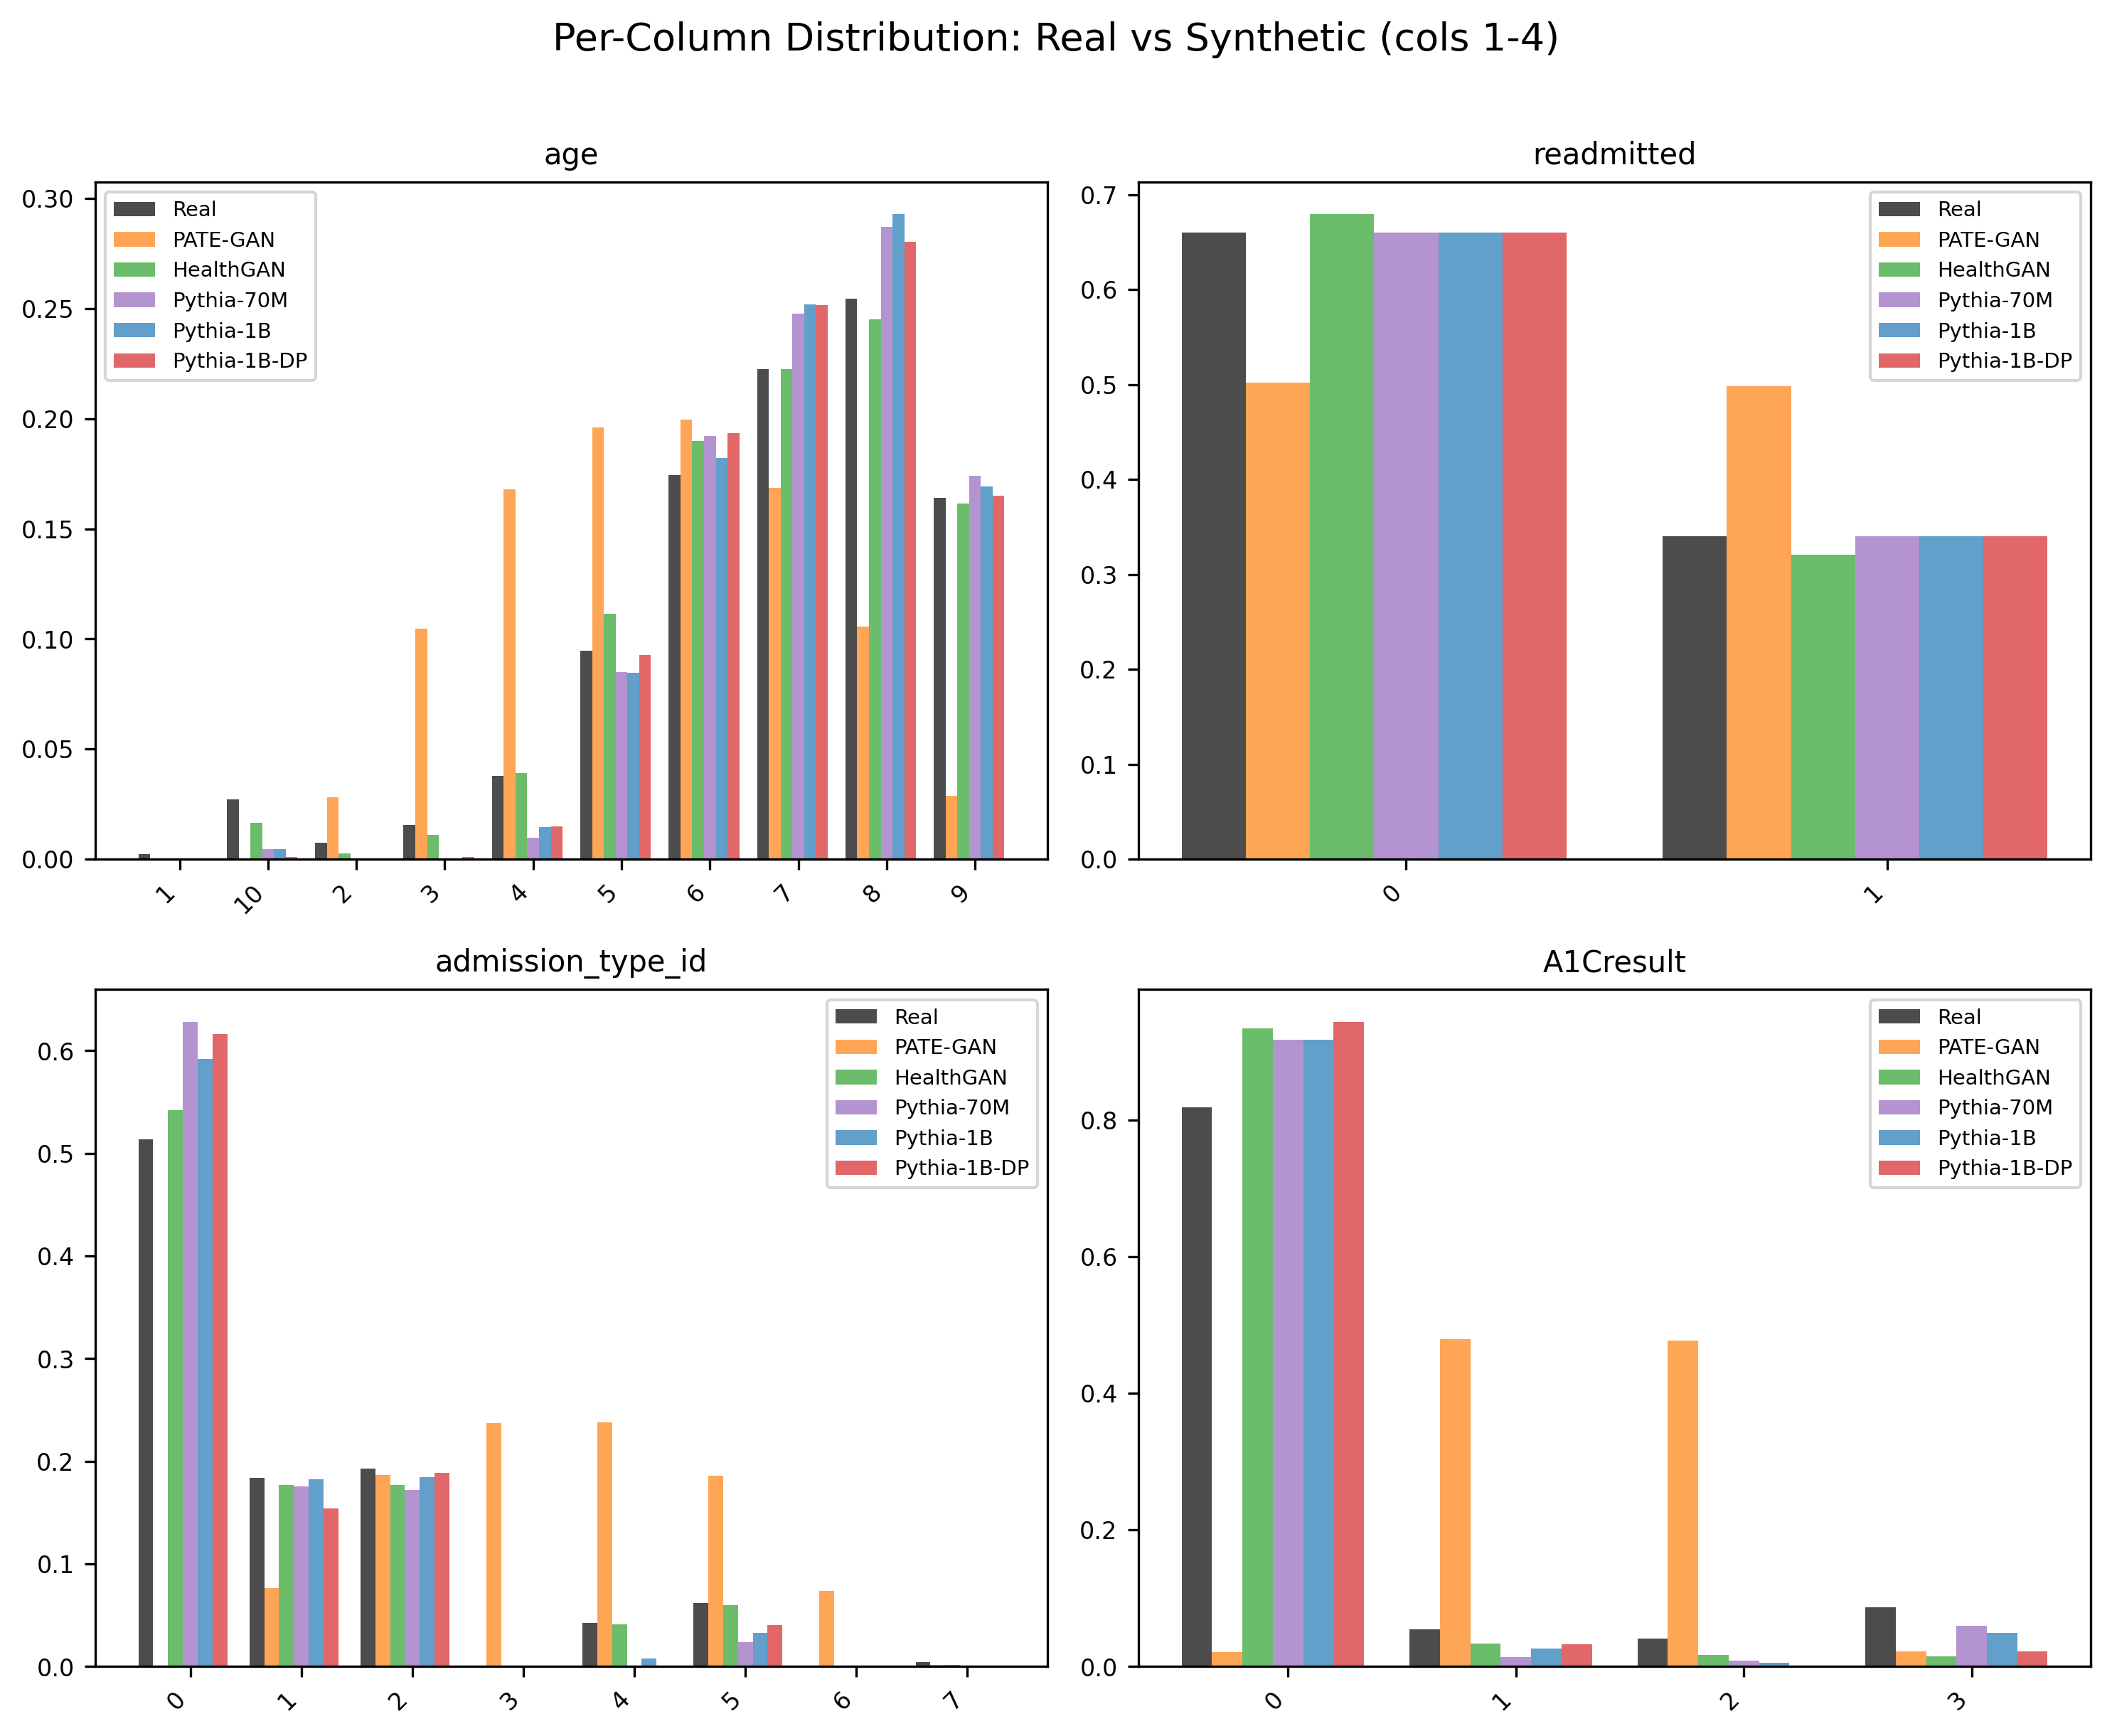
\includegraphics[width=0.90\textwidth]
{images/results/1a-per_column_distribution_reordered_1}
\caption{Representative marginal distributions for ordinal, binary, and
categorical columns, comparing the real data with five synthetic
generators. HealthGAN and the three Pythia variants closely match the real
reference, while PATE-GAN distorts the categorical marginals.}
\label{fig:rq2:marginals}
\end{figure}

\begin{figure}[H]
\centering
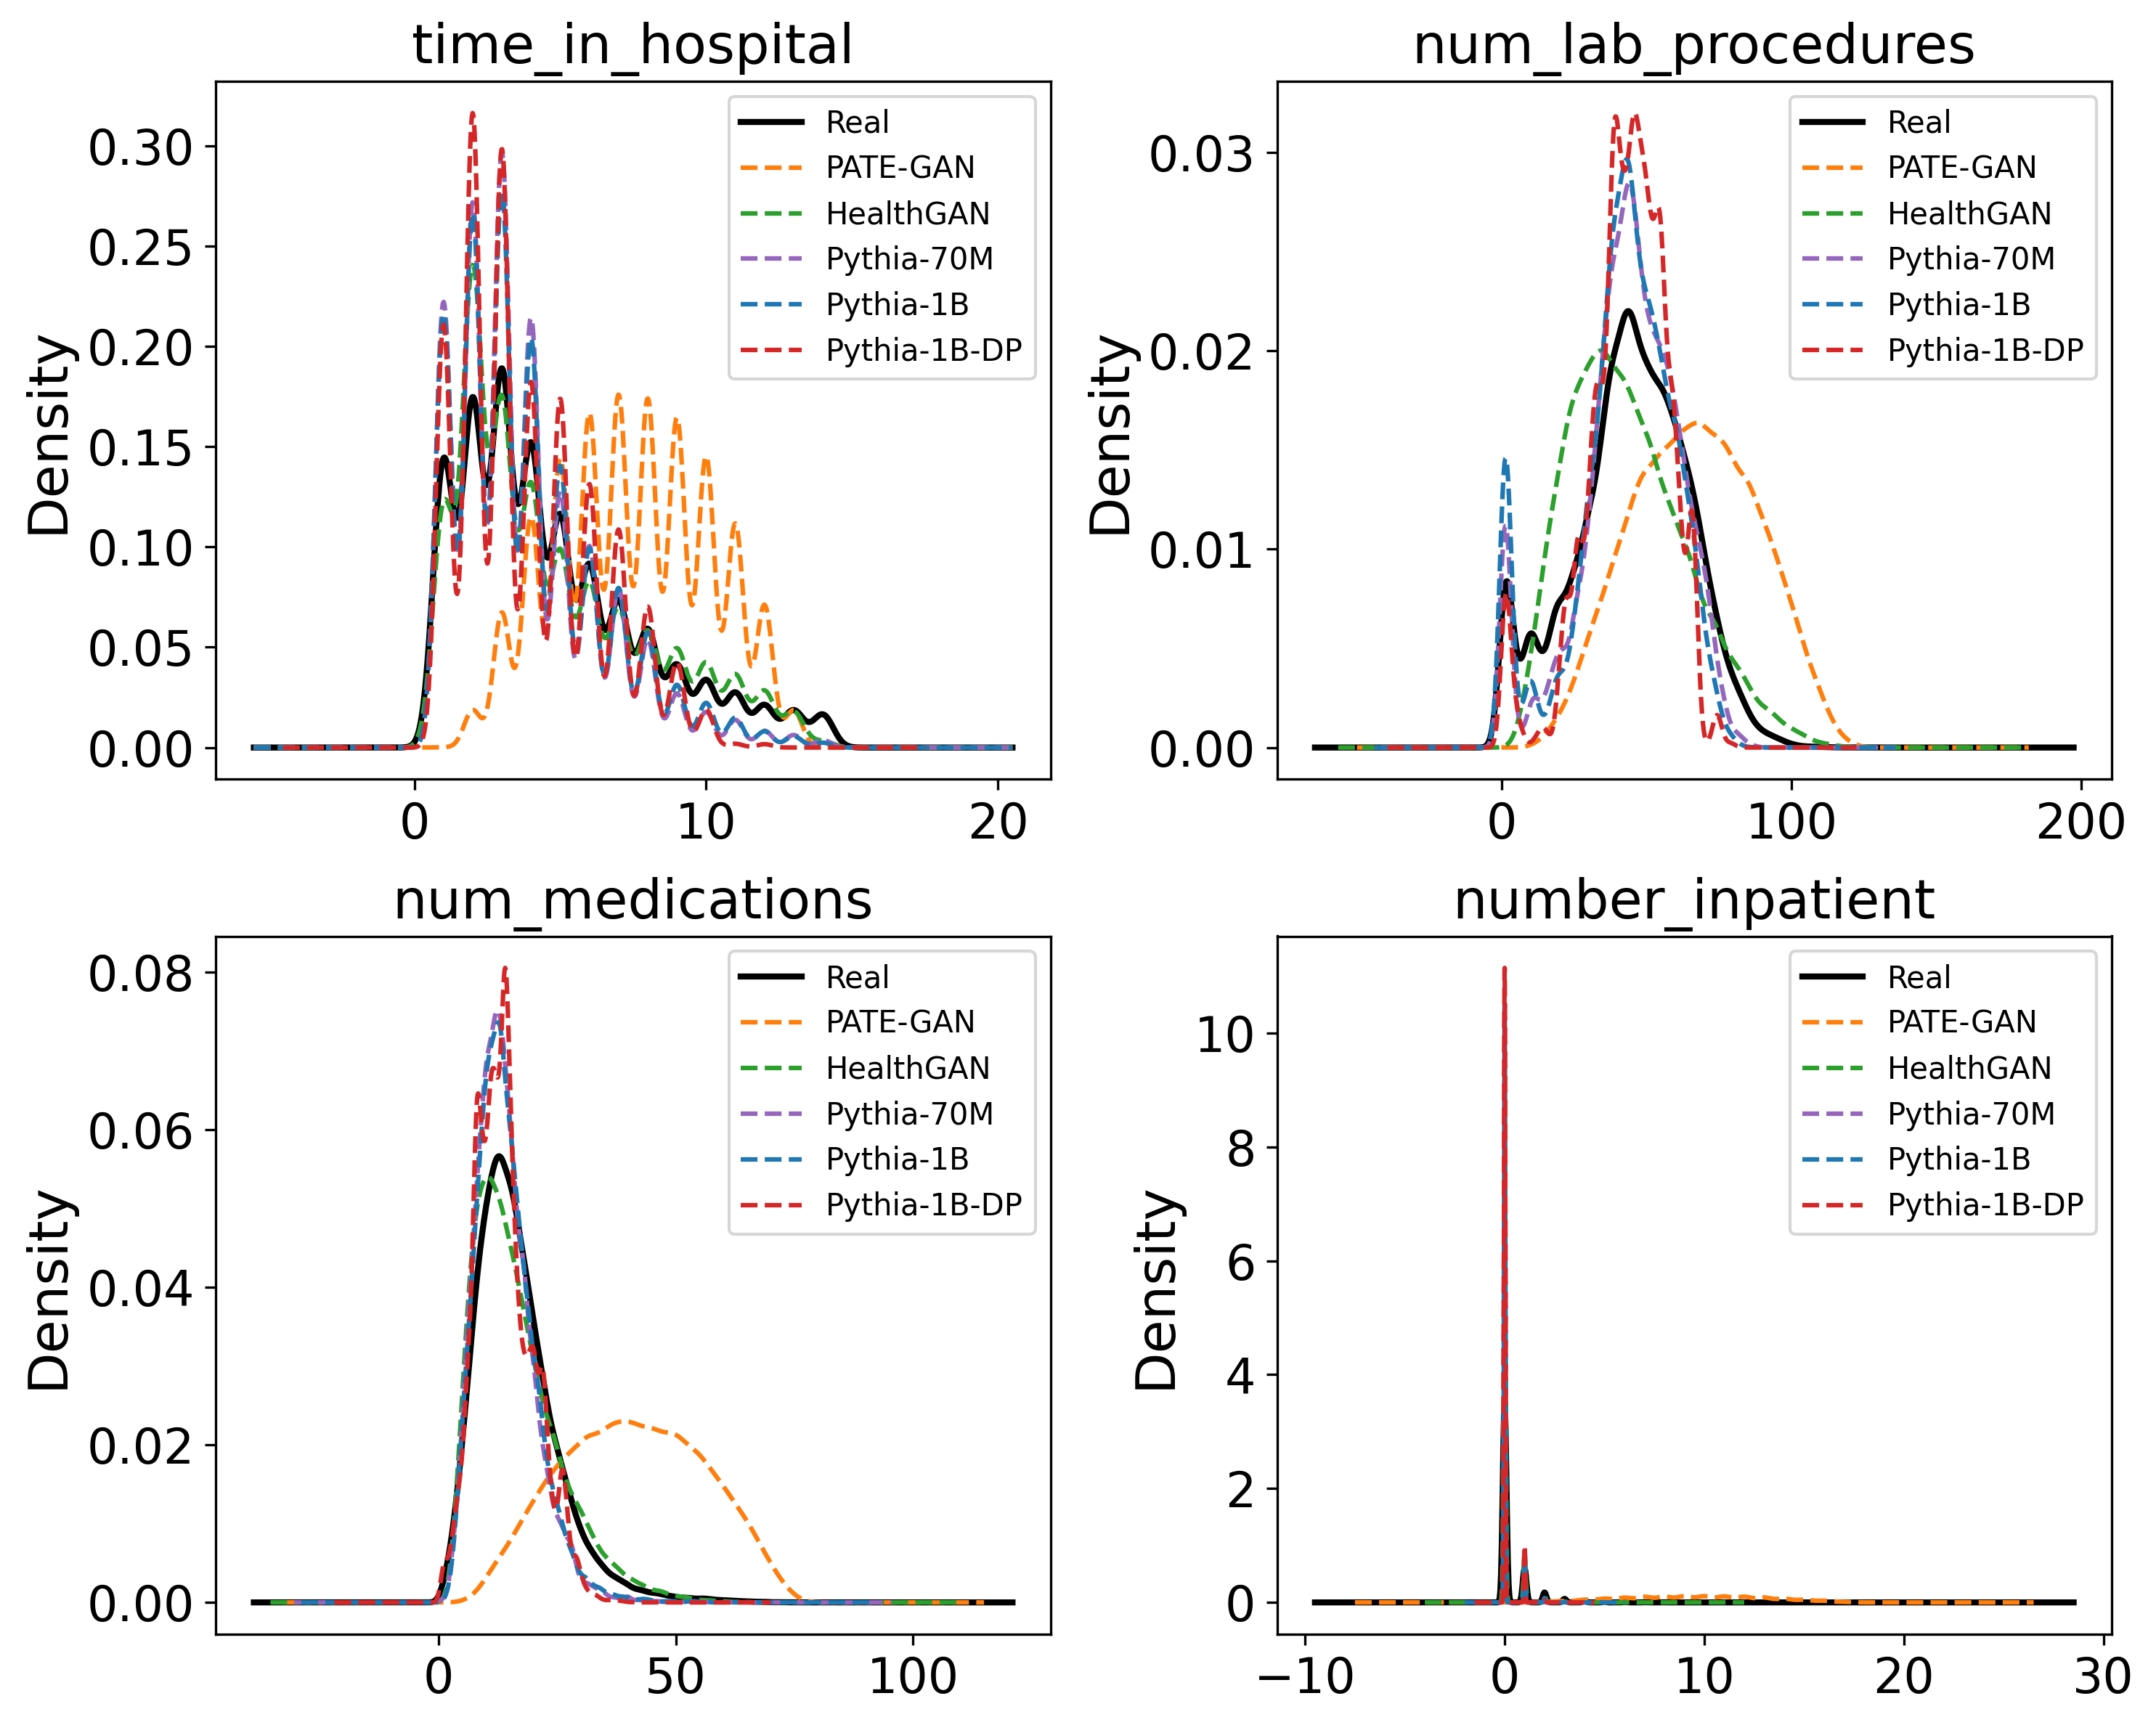
\includegraphics[width=0.90\textwidth]
{images/results/1a-per_column_distribution_reordered_2}
\caption{Representative marginal distributions for continuous
clinical-count columns, comparing the real data with five synthetic
generators. HealthGAN and the three Pythia variants closely match the real
reference, while PATE-GAN distorts the continuous marginals.}
\label{fig:rq2:marginals-continuous}
\end{figure}

Four of the five
generators, namely HealthGAN and the three Pythia variants, reproduce the
real marginals closely. Their bar charts and density curves closely match 
the real reference data for both categorical and continuous variables. 
PATE-GAN is the consistent
exception. It flattens the \emph{readmitted} distribution towards an even
split rather than the real 66:34 ratio, assigns substantial probability
mass to \emph{age} and \emph{admission\_\allowbreak type\_\allowbreak id} categories that are
rare or absent in the real data. From the other columns, we can also see that PATE-GAN's
distribution is placed mostly on either dominant categories or for continuous colmns they
are mostly smooth distribution near the median. This is the earilest sign that PATE-GAN 
is not learning the read data distribution well and is instead producing a distorted output.
The full per-column gallery for all five generators is provided in Appendix~\ref{app:distributions}.


\paragraph{Marginal and Joint Similarity Scores:}
Table~\ref{tab:rq2:ks-pcd} reduces the per-column comparison to two
headline scalars defined in
Sections~\ref{sec:eval:utility:similarity:ks}
and~\ref{sec:eval:utility:similarity:pcd}: i) mean Kolmogorov-Smirnov
(KS) statistic averaged across columns, which averages each
column's largest empirical-distribution difference, and ii) mean pairwise correlation difference (PCD),
which measures the fidelity of the joint linear-dependency structure.
The full per-column KS values behind the mean are
tabulated in Appendix~\ref{app:ks-per-column}.

Throughout the result tables, $\uparrow$ indicates that higher values are
preferable, whereas $\downarrow$ indicates that lower values are preferable.
For tables reporting $\Delta$, the sign should therefore be interpreted
relative to this direction. A positive change is favourable for $\uparrow$
metrics but unfavourable for $\downarrow$ metrics.

\begin{table}[!htbp]
\centering
\small
\caption{Mean Kolmogorov-Smirnov statistic and mean pairwise correlation
difference per generator (lower is better on both). KS is averaged over
all compared columns, PCD is the mean absolute difference between the real
and synthetic correlation matrices. The best non-trivial value in each
column is shown in bold.}
\label{tab:rq2:ks-pcd}
% Auto-generated by data_analysis.ipynb (1d). Do not edit by hand.
% Requires booktabs.
\begin{tabular}{lcc}
\toprule
Generator & Mean KS $\downarrow$ & PCD $\downarrow$ \\
\midrule
PATE-GAN & 0.5381 & 0.1142 \\
HealthGAN & \textbf{0.0480} & 0.0336 \\
Pythia-70M & 0.0856 & 0.0308 \\
Pythia-1B & 0.0805 & \textbf{0.0206} \\
Pythia-1B-DP & 0.0992 & 0.0466 \\
\bottomrule
\end{tabular}

\end{table}

The two scalars confirm the visual reading. HealthGAN attains the lowest
mean KS and Pythia-1B the lowest PCD, with the four non-PATE generators all falling
in a narrow band (mean KS $0.048$-$0.099$; PCD $0.021$-$0.047$).
PATE-GAN is more than an order of magnitude worse on the marginal axis
(mean KS $0.5381$) and three to five times worse on the joint axis
(PCD $0.1142$). Thus places it in a separate regime from every other
generator. Within the LLM family, the differentially private variant is
modestly worse than its non-private counterpart on both axes (mean KS
$0.0992$ vs.\ $0.0805$; PCD $0.0466$ vs.\ $0.0206$). it is an early indication
of the differential-privacy utility cost quantified within-family in
Section~\ref{sec:results:rq3:llm-toggle}.

\paragraph{Correlation Structure:}
Figure~\ref{fig:rq2:corrheat} contrasts the correlation-difference
heatmaps (real minus synthetic correlation matrix) of the two
joint-similarity extremes. PATE-GAN exhibits dense blocks of large
residual correlation across the clinical and medication columns,
indicating that the dependency structure of its output departs
substantially from the real data. Pythia-1B is near-uniformly pale,
indicating that most pairwise correlations are reproduced to within a
small residual. The corresponding heatmaps for the remaining three
generators (HealthGAN, Pythia-70M, and Pythia-1B-DP), consistent with
the PCD ordering of Table~\ref{tab:rq2:ks-pcd}, are collected in
Appendix~\ref{app:corrheat}.

\begin{table}[H]
\centering
\caption{Mean Absolute Correlation Difference across models.}
\label{tab:mean-absolute-correlation-difference}
\begin{tabular}{lc}
\hline
\textbf{Model} & \textbf{Mean Absolute Correlation Difference} \\
\hline
PATE-GAN      & 0.1142 \\
HealthGAN     & 0.0336 \\
Pythia-70M    & 0.0308 \\
Pythia-1B     & \textbf{0.0206} \\
Pythia-1B-DP  & 0.0466 \\
\hline
\end{tabular}
\end{table}

The quantitative results are consistent with the patterns observed in the
correlation-difference heatmaps. Pythia-1B achieves the lowest mean
absolute correlation difference (0.0206), indicating the closest
reproduction of the real data's correlation structure, whereas
PATE-GAN records the highest difference (0.1142). HealthGAN and
Pythia-70M perform comparably, while the higher value of Pythia-1B-DP
suggests that differential privacy reduces correlation fidelity.

\begin{figure}[H]
\centering

\begin{subfigure}{\textwidth}
\centering
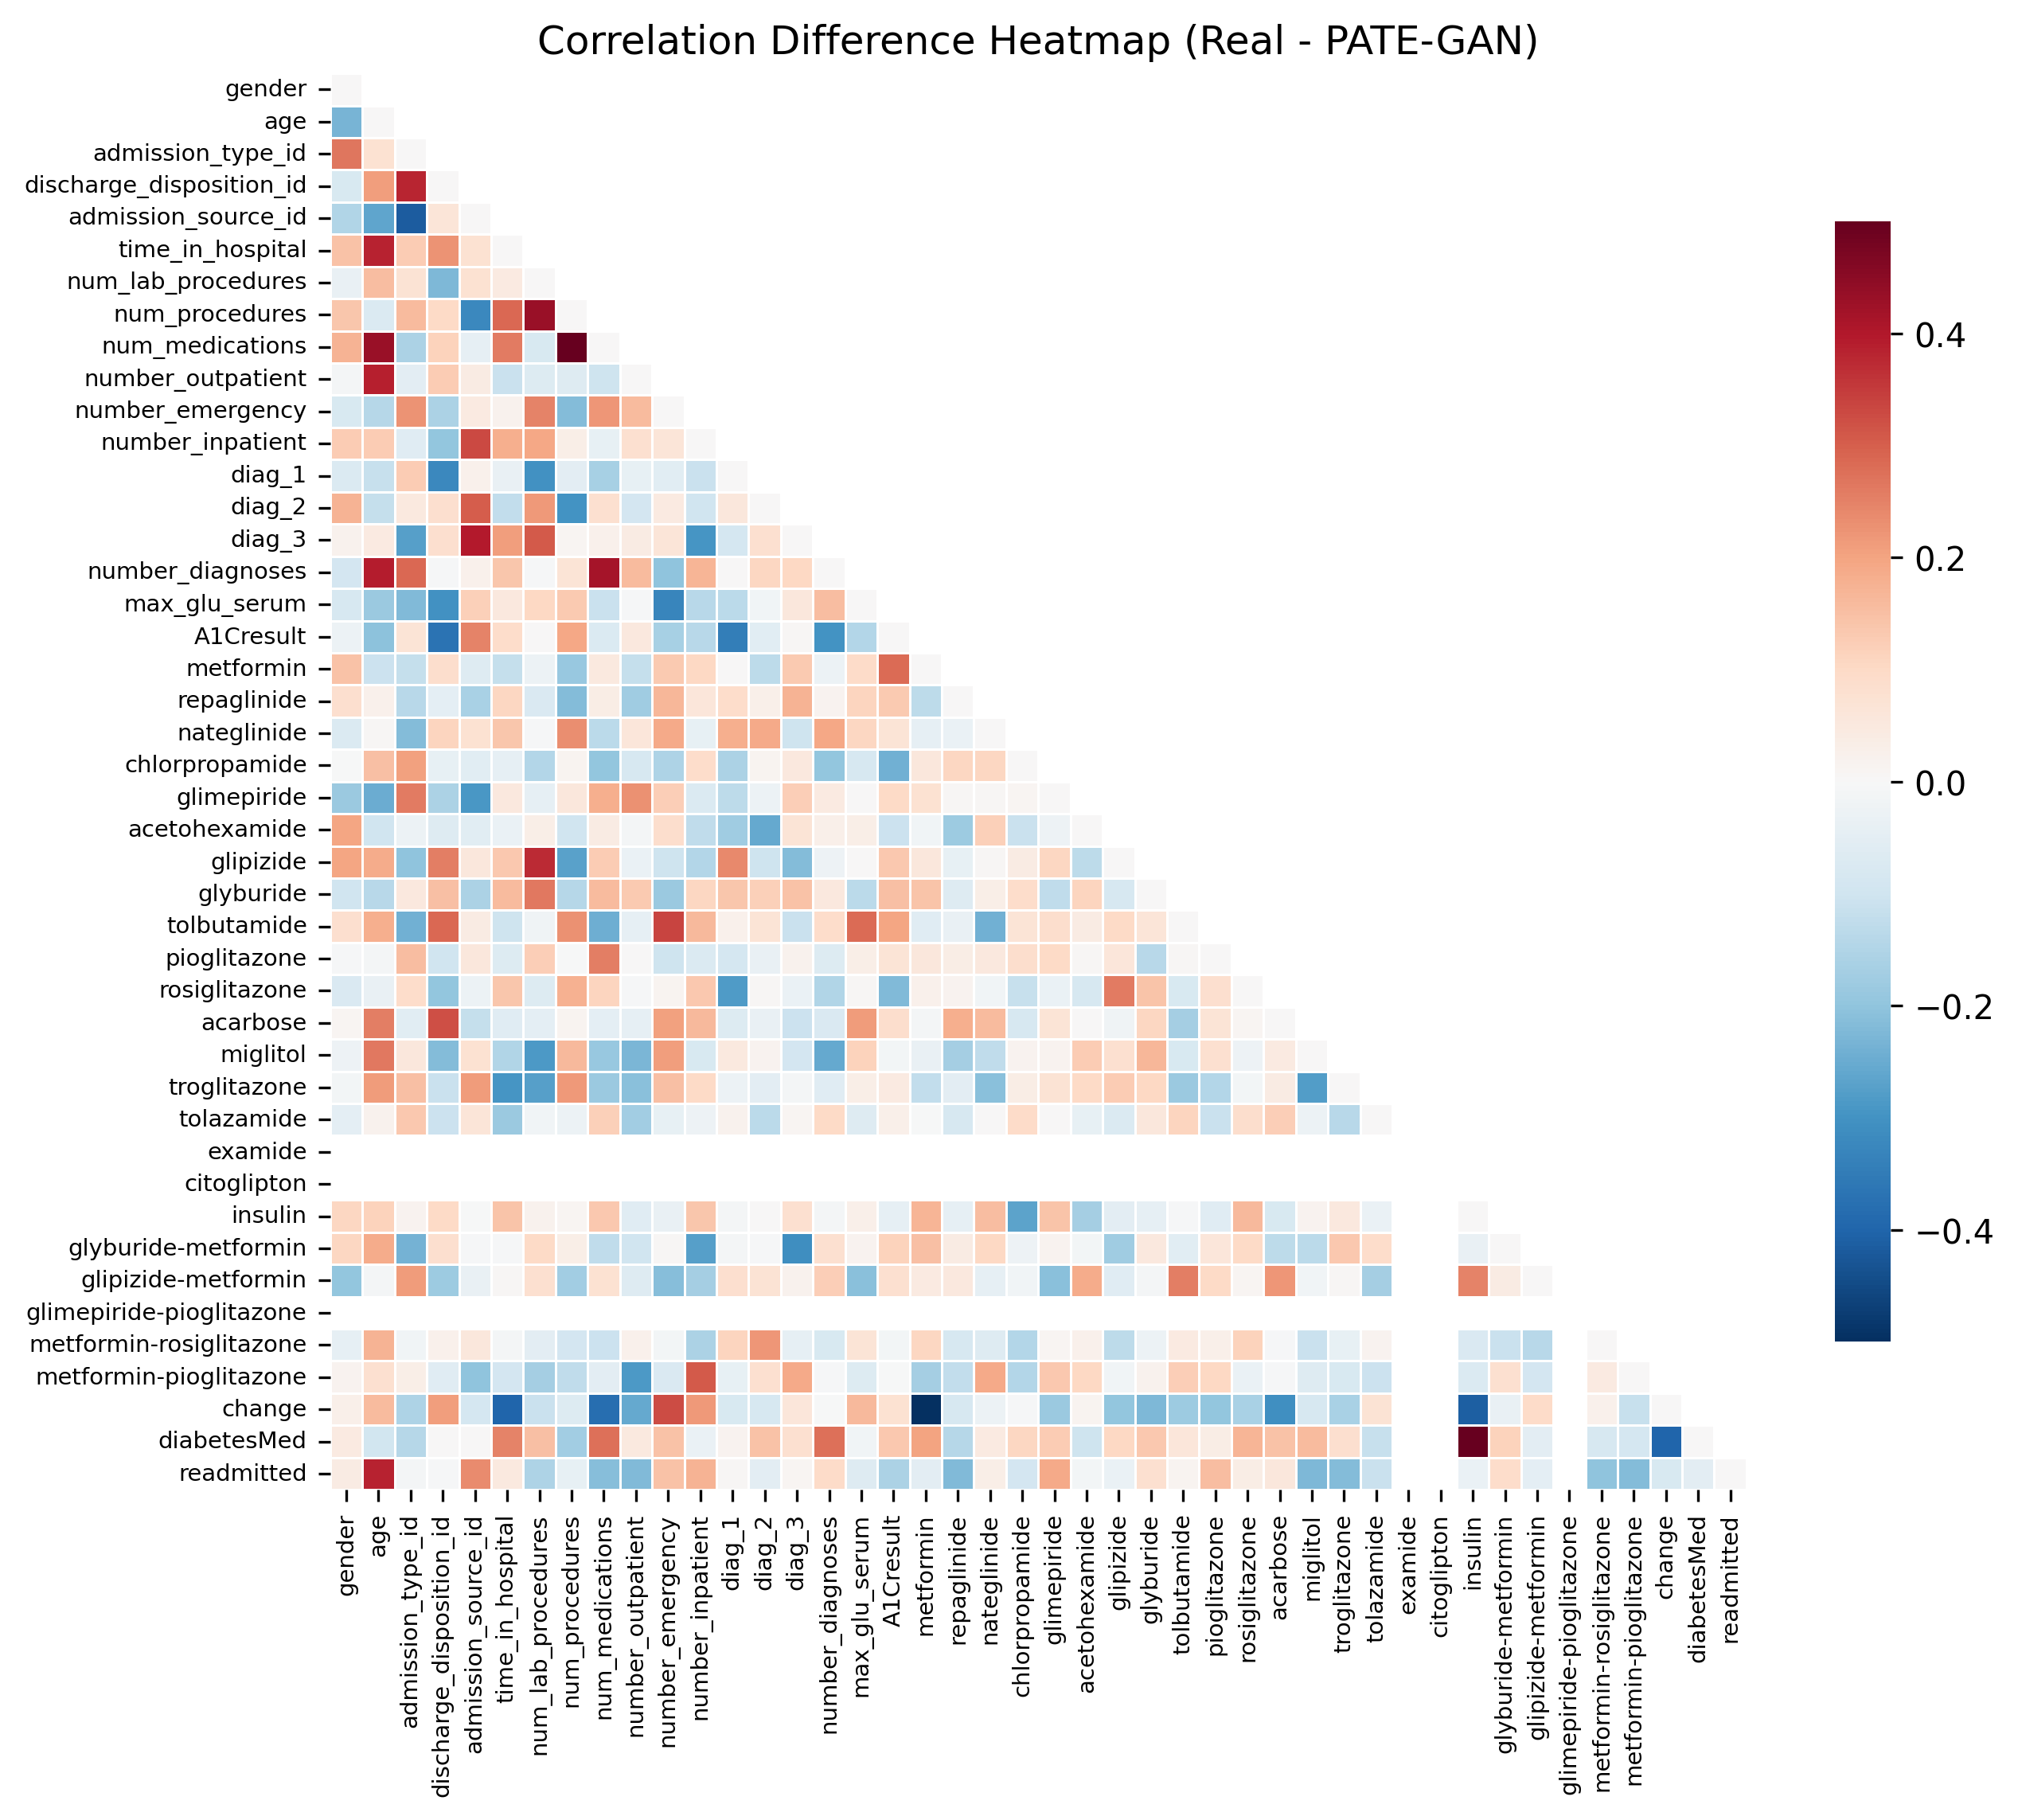
\includegraphics[
    width=\textwidth,
    height=0.45\textheight,
    keepaspectratio
]{images/results/1c-corr_diff_heatmap_1}
\caption{PATE-GAN.}
\end{subfigure}

\vspace{1em}

\begin{subfigure}{\textwidth}
\centering
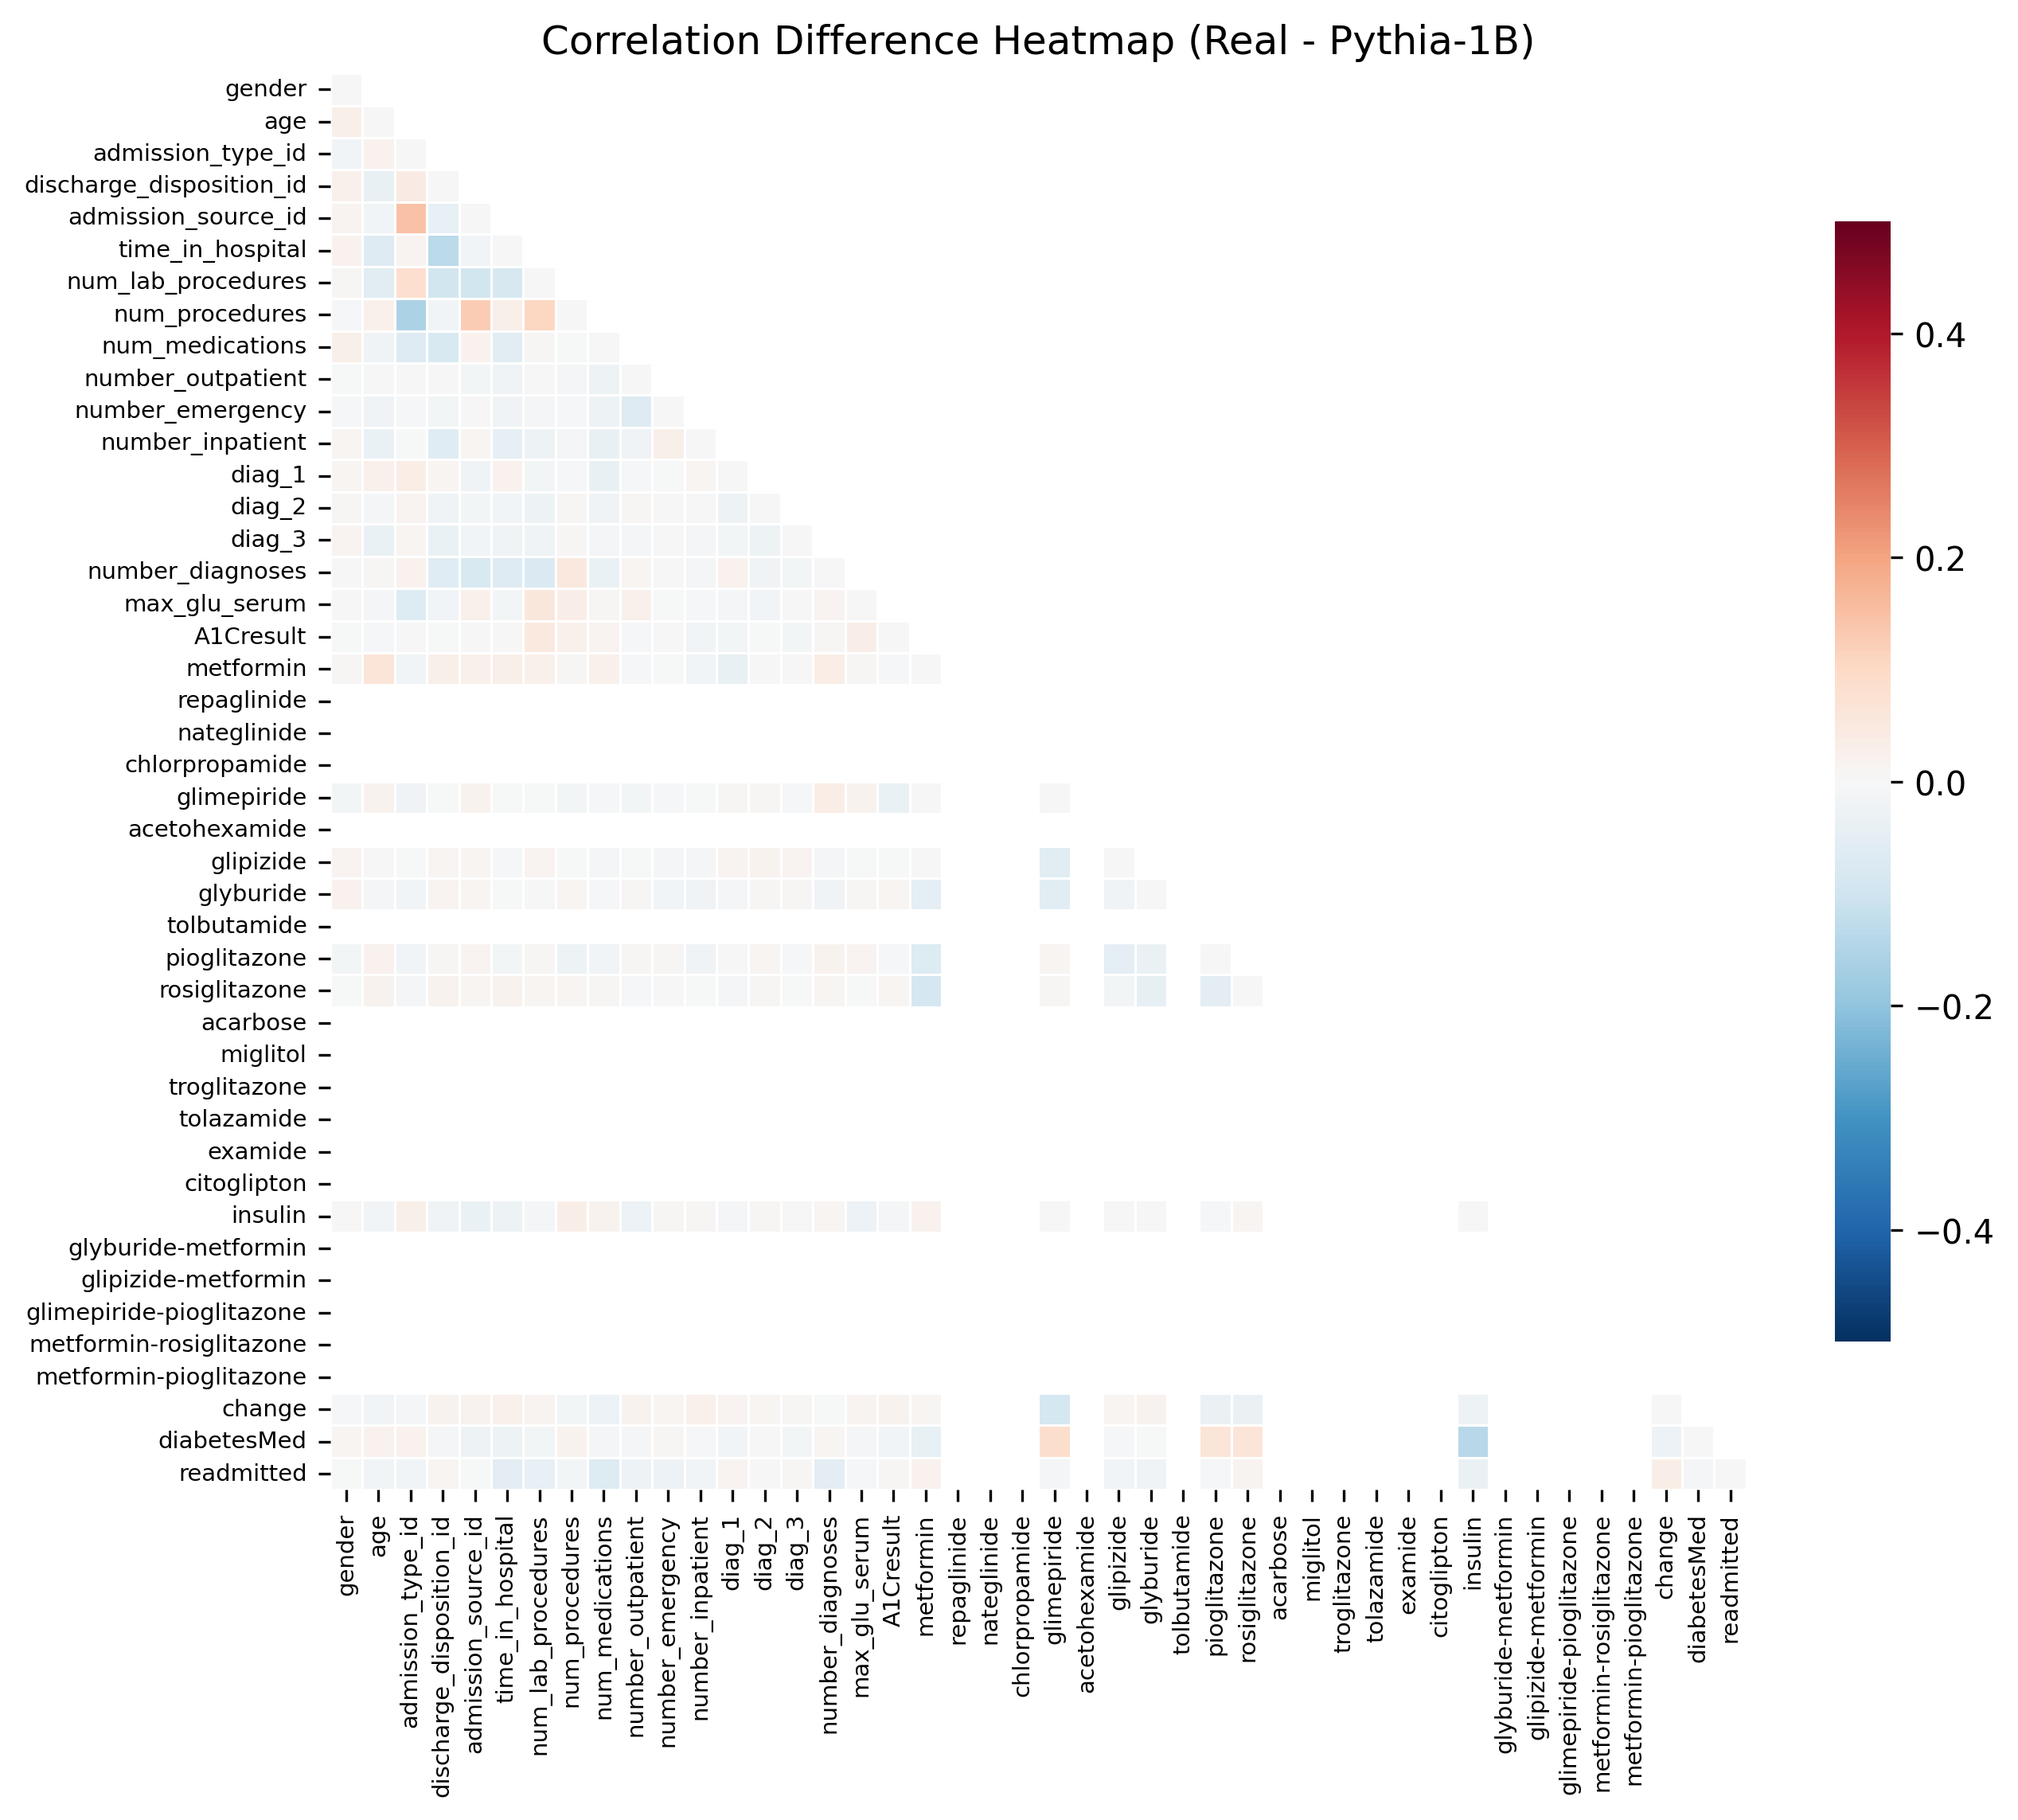
\includegraphics[
    width=\textwidth,
    height=0.45\textheight,
    keepaspectratio
]{images/results/1c-corr_diff_heatmap_4}
\caption{Pythia-1B.}
\end{subfigure}

\caption{Correlation-difference heatmaps comparing the real and synthetic
correlation matrices. PATE-GAN shows large residual correlations, while
Pythia-1B more closely reproduces the real correlation structure.}
\label{fig:rq2:corrheat}
\end{figure}

\paragraph{PCA-Based Manifold Overlap:}
Figure~\ref{fig:rq2:pca} projects the real and synthetic records onto the
first two principal components estimated from the combined real-plus-synthetic table
(Section~\ref{sec:eval:utility:similarity:pca}). The real cloud and four
of the five synthetic clouds occupy a common region of the projected
space, whereas PATE-GAN forms a disjoint cluster displaced along the
first principal component. The projection therefore represents at the
joint level what the marginal and correlation views establish separately.
PATE-GAN’s samples differ from the real-data distribution, 
while those of the other four generators align closely with it. This also 
aligns with our previous observation of PATE-GAN.
\begin{figure}[H]
\centering
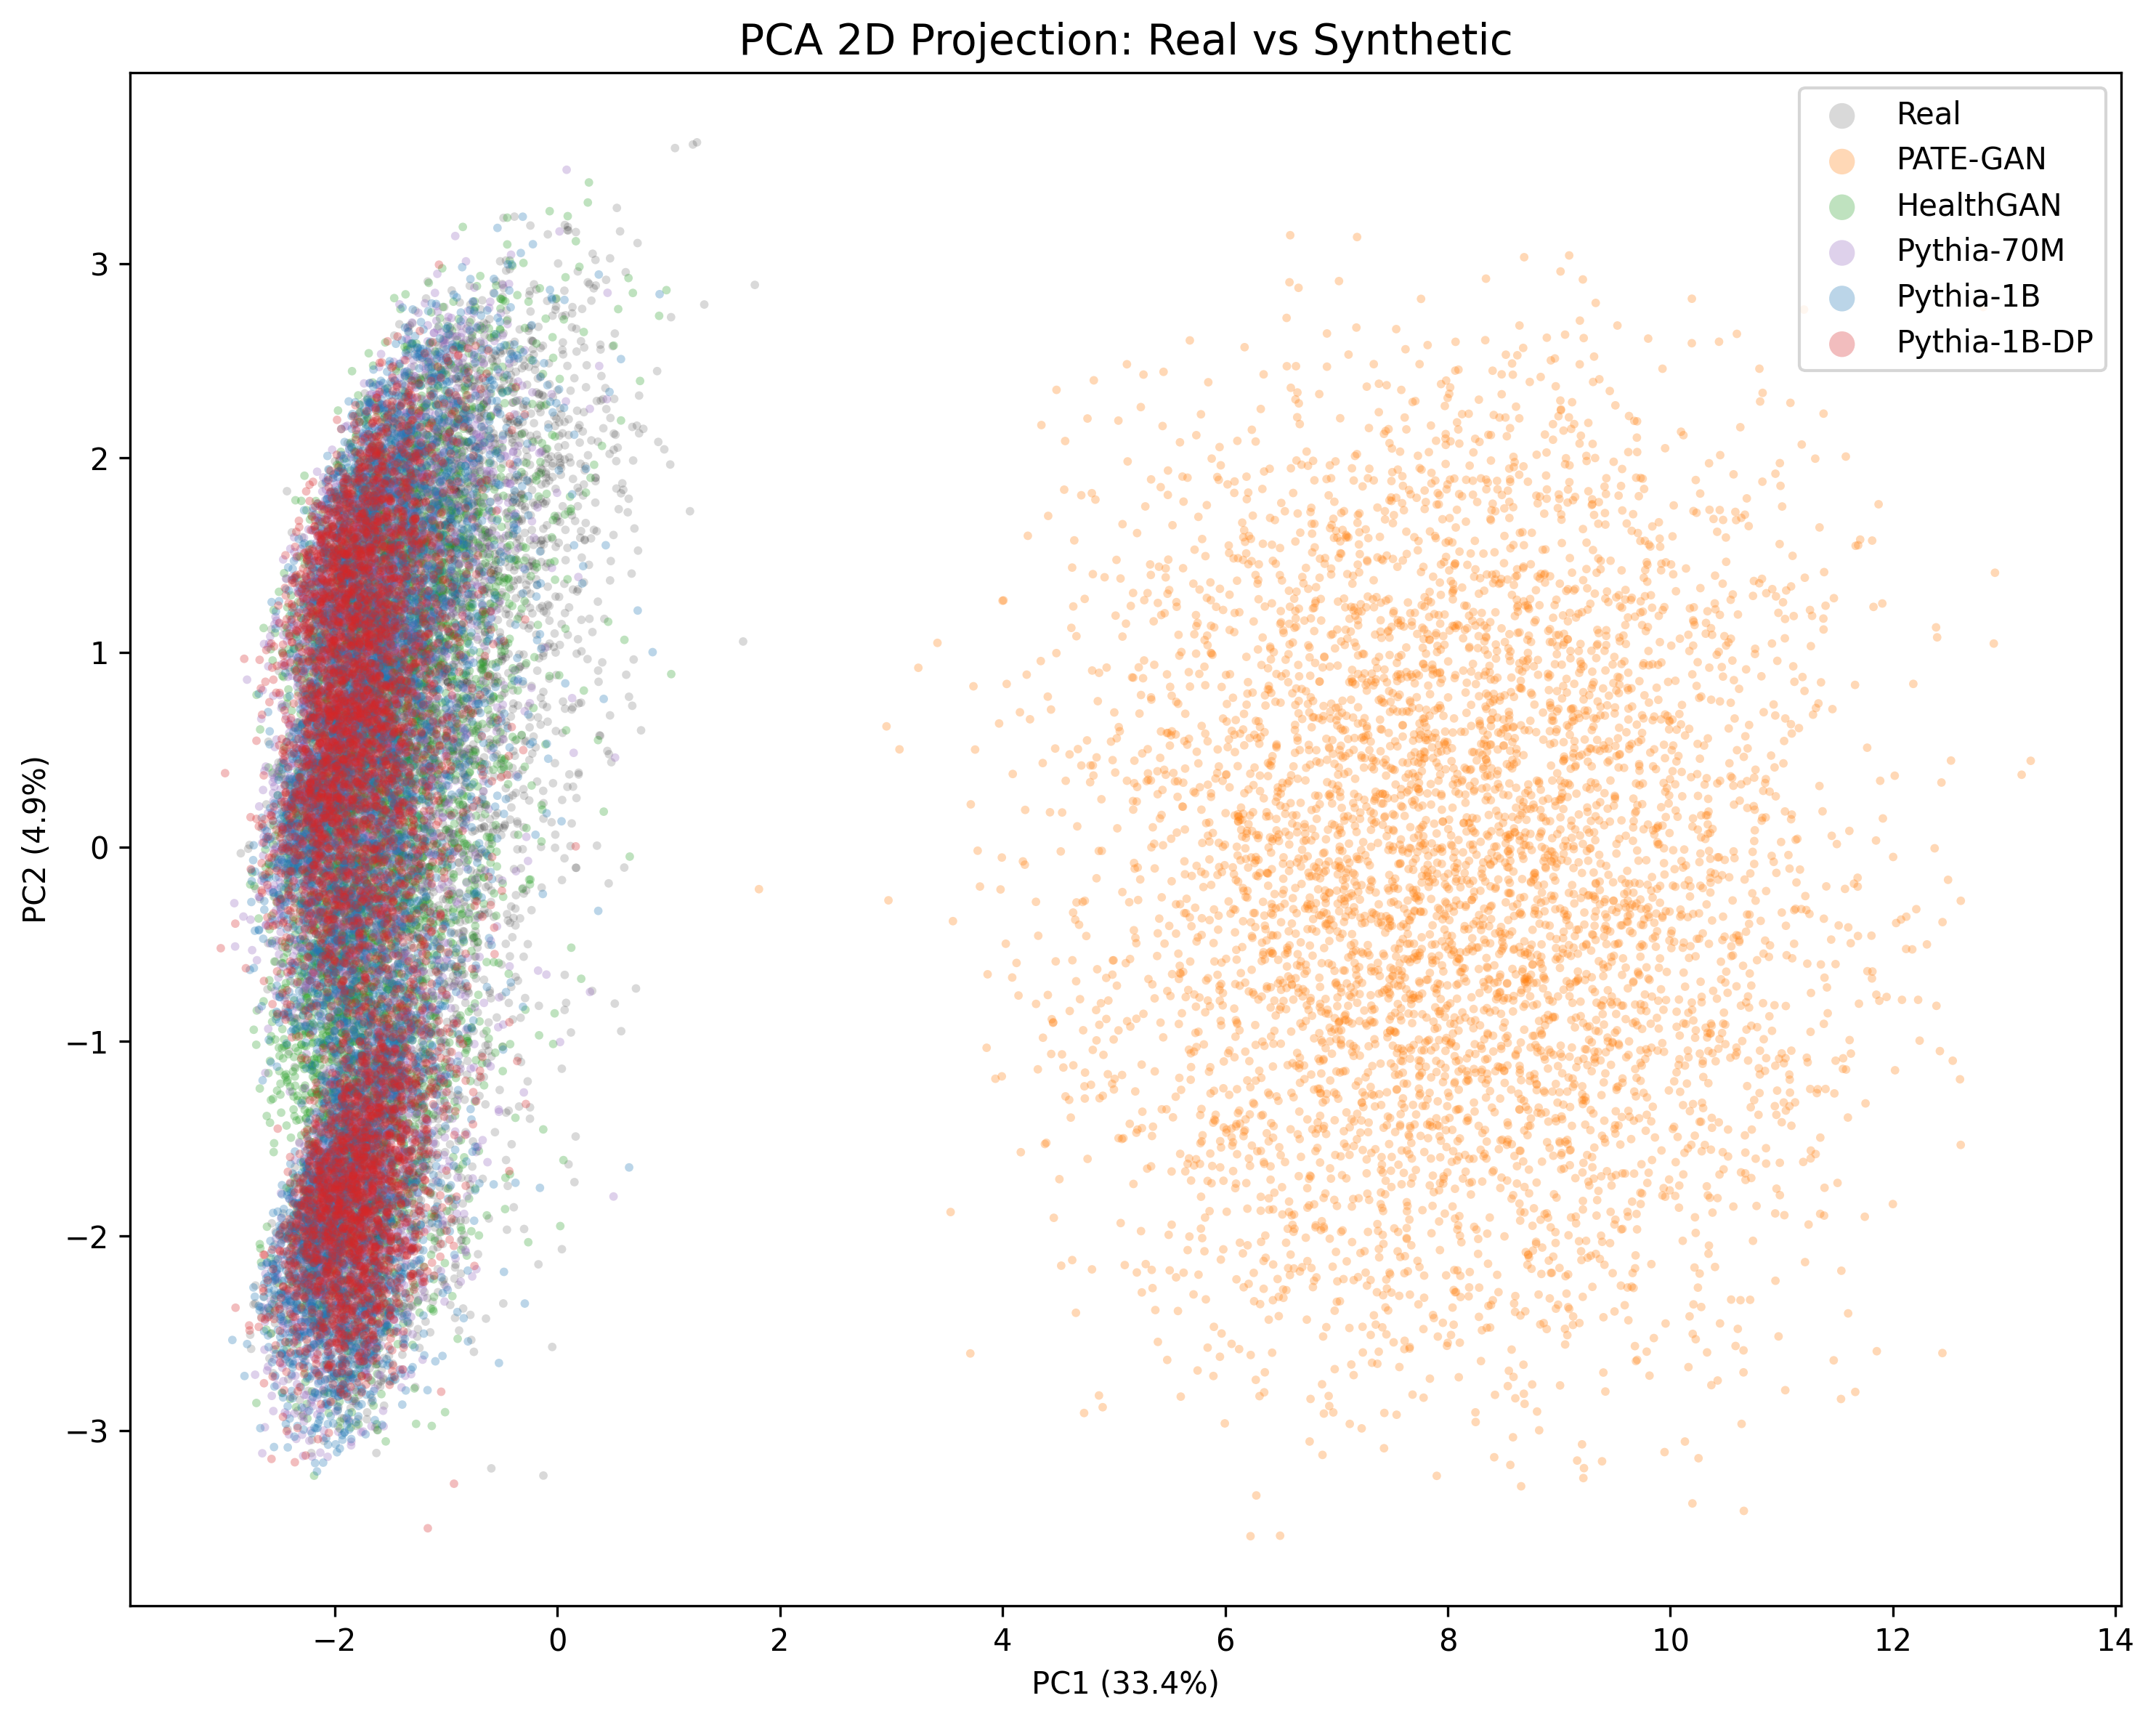
\includegraphics[width=0.85\textwidth]{images/results/1e-pca_projection}
\caption{Two-dimensional PCA projection onto principal components estimated
from the combined real-plus-synthetic table. Four generators overlap the
real cloud; PATE-GAN is displaced into a disjoint region along the first
principal component.}
\label{fig:rq2:pca}
\end{figure}

\subsubsection{Predictive Performance}
\label{sec:results:rq2:utility:predictive}

Predictive utility is measured under the Train-on-Synthetic,
Test-on-Real (TSTR) protocol defined in
Section~\ref{sec:eval:utility:predictive:tstr}. A classifier is trained
on each synthetic table and evaluated on the held-out real test split
($n = 14{,}304$) with \emph{readmitted} as the binary target. The
Train-on-Real, Test-on-Real (TRTR) model provides the upper-bound
reference. Three downstream classifiers are reported
(Section~\ref{sec:eval:utility:predictive:classifiers}). Gradient
Boosting is taken as the headline model, with Logistic Regression and
Random Forest included.

\paragraph{Class-Balance Diagnostic:}
Before interpreting the threshold-dependent classifier metrics, the
positive-class prevalence of the binary readmission target was checked
across real and synthetic train/test splits. The real train and test splits
both have a readmission rate of approximately $0.340$. PATE-GAN
substantially over-produces the positive class in both synthetic splits
($0.498$ train, $0.507$ test), whereas HealthGAN remains close to the real
prevalence and the Pythia variants match the real split proportions by
construction through class-conditioned generation. This diagnostic is not a
predictive-utility metric, but it helps interpret F1, precision, and recall,
because target-prevalence shifts can change classifier operating behaviour
independently of feature quality. The full class-balance table and
TRTR/TSTR/TRTS/TSTS AUC-ROC matrix are reported in
Appendix~\ref{app:class-balance}.

\paragraph{TSTR Classifier Performance:}
Table~\ref{tab:rq2:tstr} presents the TSTR results for every combination
of training source and classifier. Models trained on real data are
included as a reference. Based on Gradient-Boosting AUC-ROC, Pythia-1B
achieves the best synthetic-data result $(0.6818)$, followed by
Pythia-70M, HealthGAN, Pythia-1B-DP,
and PATE-GAN. The real-trained model achieves $0.7008$.
Pythia-1B therefore retains approximately $97\%$ of the real-data
AUC-ROC, while PATE-GAN performs only slightly above the chance level
of $0.5$. This means that Pythia-1B preserves most of the predictive
information available in the real data, whereas PATE-GAN preserves
little useful discriminatory information.

\begin{table}[H]
\centering
\small
\caption{Train-on-Synthetic, Test-on-Real (TSTR) utility for all five
generators and the Train-on-Real (TRTR) reference, evaluated on the real
held-out split ($n = 14{,}304$) with \emph{readmitted} as the target.
The highest synthetic Gradient-Boosting AUC-ROC is shown in bold.}
\label{tab:rq2:tstr}
% Auto-generated by data_analysis.ipynb (2a). Do not edit by hand.
% Requires booktabs.
\begin{tabular}{llccccc}
\toprule
Train Source & Classifier & AUC-ROC & F1 & Accuracy & Precision & Recall \\
\midrule
Real (TRTR) & Logistic Regression & 0.6670 & 0.2837 & 0.6804 & 0.5974 & 0.1860 \\
Real (TRTR) & Random Forest & 0.6790 & 0.3648 & 0.6895 & 0.6000 & 0.2620 \\
Real (TRTR) & Gradient Boosting & 0.7008 & 0.3668 & 0.6962 & 0.6301 & 0.2587 \\
\midrule
PATE-GAN & Logistic Regression & 0.5079 & 0.0417 & 0.6528 & 0.3407 & 0.0222 \\
PATE-GAN & Random Forest & 0.5018 & 0.0246 & 0.6567 & 0.3669 & 0.0127 \\
PATE-GAN & Gradient Boosting & 0.5108 & 0.0093 & 0.6583 & 0.3433 & 0.0047 \\
\midrule
HealthGAN & Logistic Regression & 0.6130 & 0.3889 & 0.6651 & 0.5128 & 0.3132 \\
HealthGAN & Random Forest & 0.6153 & 0.3826 & 0.6655 & 0.5142 & 0.3046 \\
HealthGAN & Gradient Boosting & 0.6312 & 0.3824 & 0.6720 & 0.5321 & 0.2984 \\
\midrule
Pythia-70M & Logistic Regression & 0.6573 & 0.5035 & 0.6337 & 0.4671 & 0.5460 \\
Pythia-70M & Random Forest & 0.6588 & 0.4966 & 0.6442 & 0.4787 & 0.5158 \\
Pythia-70M & Gradient Boosting & 0.6634 & 0.5005 & 0.6408 & 0.4749 & 0.5290 \\
\midrule
Pythia-1B & Logistic Regression & 0.6613 & 0.4984 & 0.6393 & 0.4730 & 0.5267 \\
Pythia-1B & Random Forest & 0.6682 & 0.5048 & 0.6523 & 0.4896 & 0.5210 \\
Pythia-1B & Gradient Boosting & \textbf{0.6818} & 0.5036 & 0.6569 & 0.4959 & 0.5115 \\
\midrule
Pythia-1B-DP & Logistic Regression & 0.5868 & 0.2509 & 0.6477 & 0.4535 & 0.1734 \\
Pythia-1B-DP & Random Forest & 0.5823 & 0.2369 & 0.6456 & 0.4426 & 0.1617 \\
Pythia-1B-DP & Gradient Boosting & 0.5827 & 0.2714 & 0.6389 & 0.4327 & 0.1977 \\
\bottomrule
\end{tabular}

\end{table}

The F1 scores show a different pattern. HealthGAN and the two
non-private Pythia models exceed the real-trained F1 score of $0.3668$,
with both Pythia models achieving approximately $0.50$. For the
non-private Pythia models, recall increases from approximately $0.26$
to between $0.51$ and $0.53$, while precision decreases from $0.63$
to between $0.47$ and $0.50$. This means that their higher F1 scores
result from identifying more readmitted patients, but at the cost of
producing more false-positive predictions. Their lower AUC-ROC values
show that this does not represent better overall discrimination than
the real-trained model.

Pythia-1B-DP achieves a lower F1 score of $0.2714$. PATE-GAN performs
poorly on both measures. Its Gradient-Boosting F1 score of $0.0093$ and
recall of $0.0047$ show that the classifier rarely predicts the positive
class. This means that differential privacy reduces the predictive
utility of Pythia-1B in this evaluation, while PATE-GAN produces
synthetic data with very limited usefulness for the readmission task.
Overall, AUC-ROC and F1 describe different aspects of predictive
utility, consistent with Table~\ref{tab:rq1-coverage}.


\paragraph{ROC Curves:}
Figure~\ref{fig:rq2:roc} overlays the Gradient-Boosting ROC curves of all
five generators against the real reference. The curves recover the AUC
ordering of Table~\ref{tab:rq2:tstr} visually. The real curve (AUC
$0.701$) has the highest AUC. Pythia-1B ($0.682$) and Pythia-70M
($0.663$) lie just beneath it. HealthGAN ($0.631$) is lower and then Pythia-1B-DP
($0.583$). PATE-GAN ($0.511$) tracks the chance diagonal
across almost the entire false-positive range.

\begin{figure}[H]
\centering
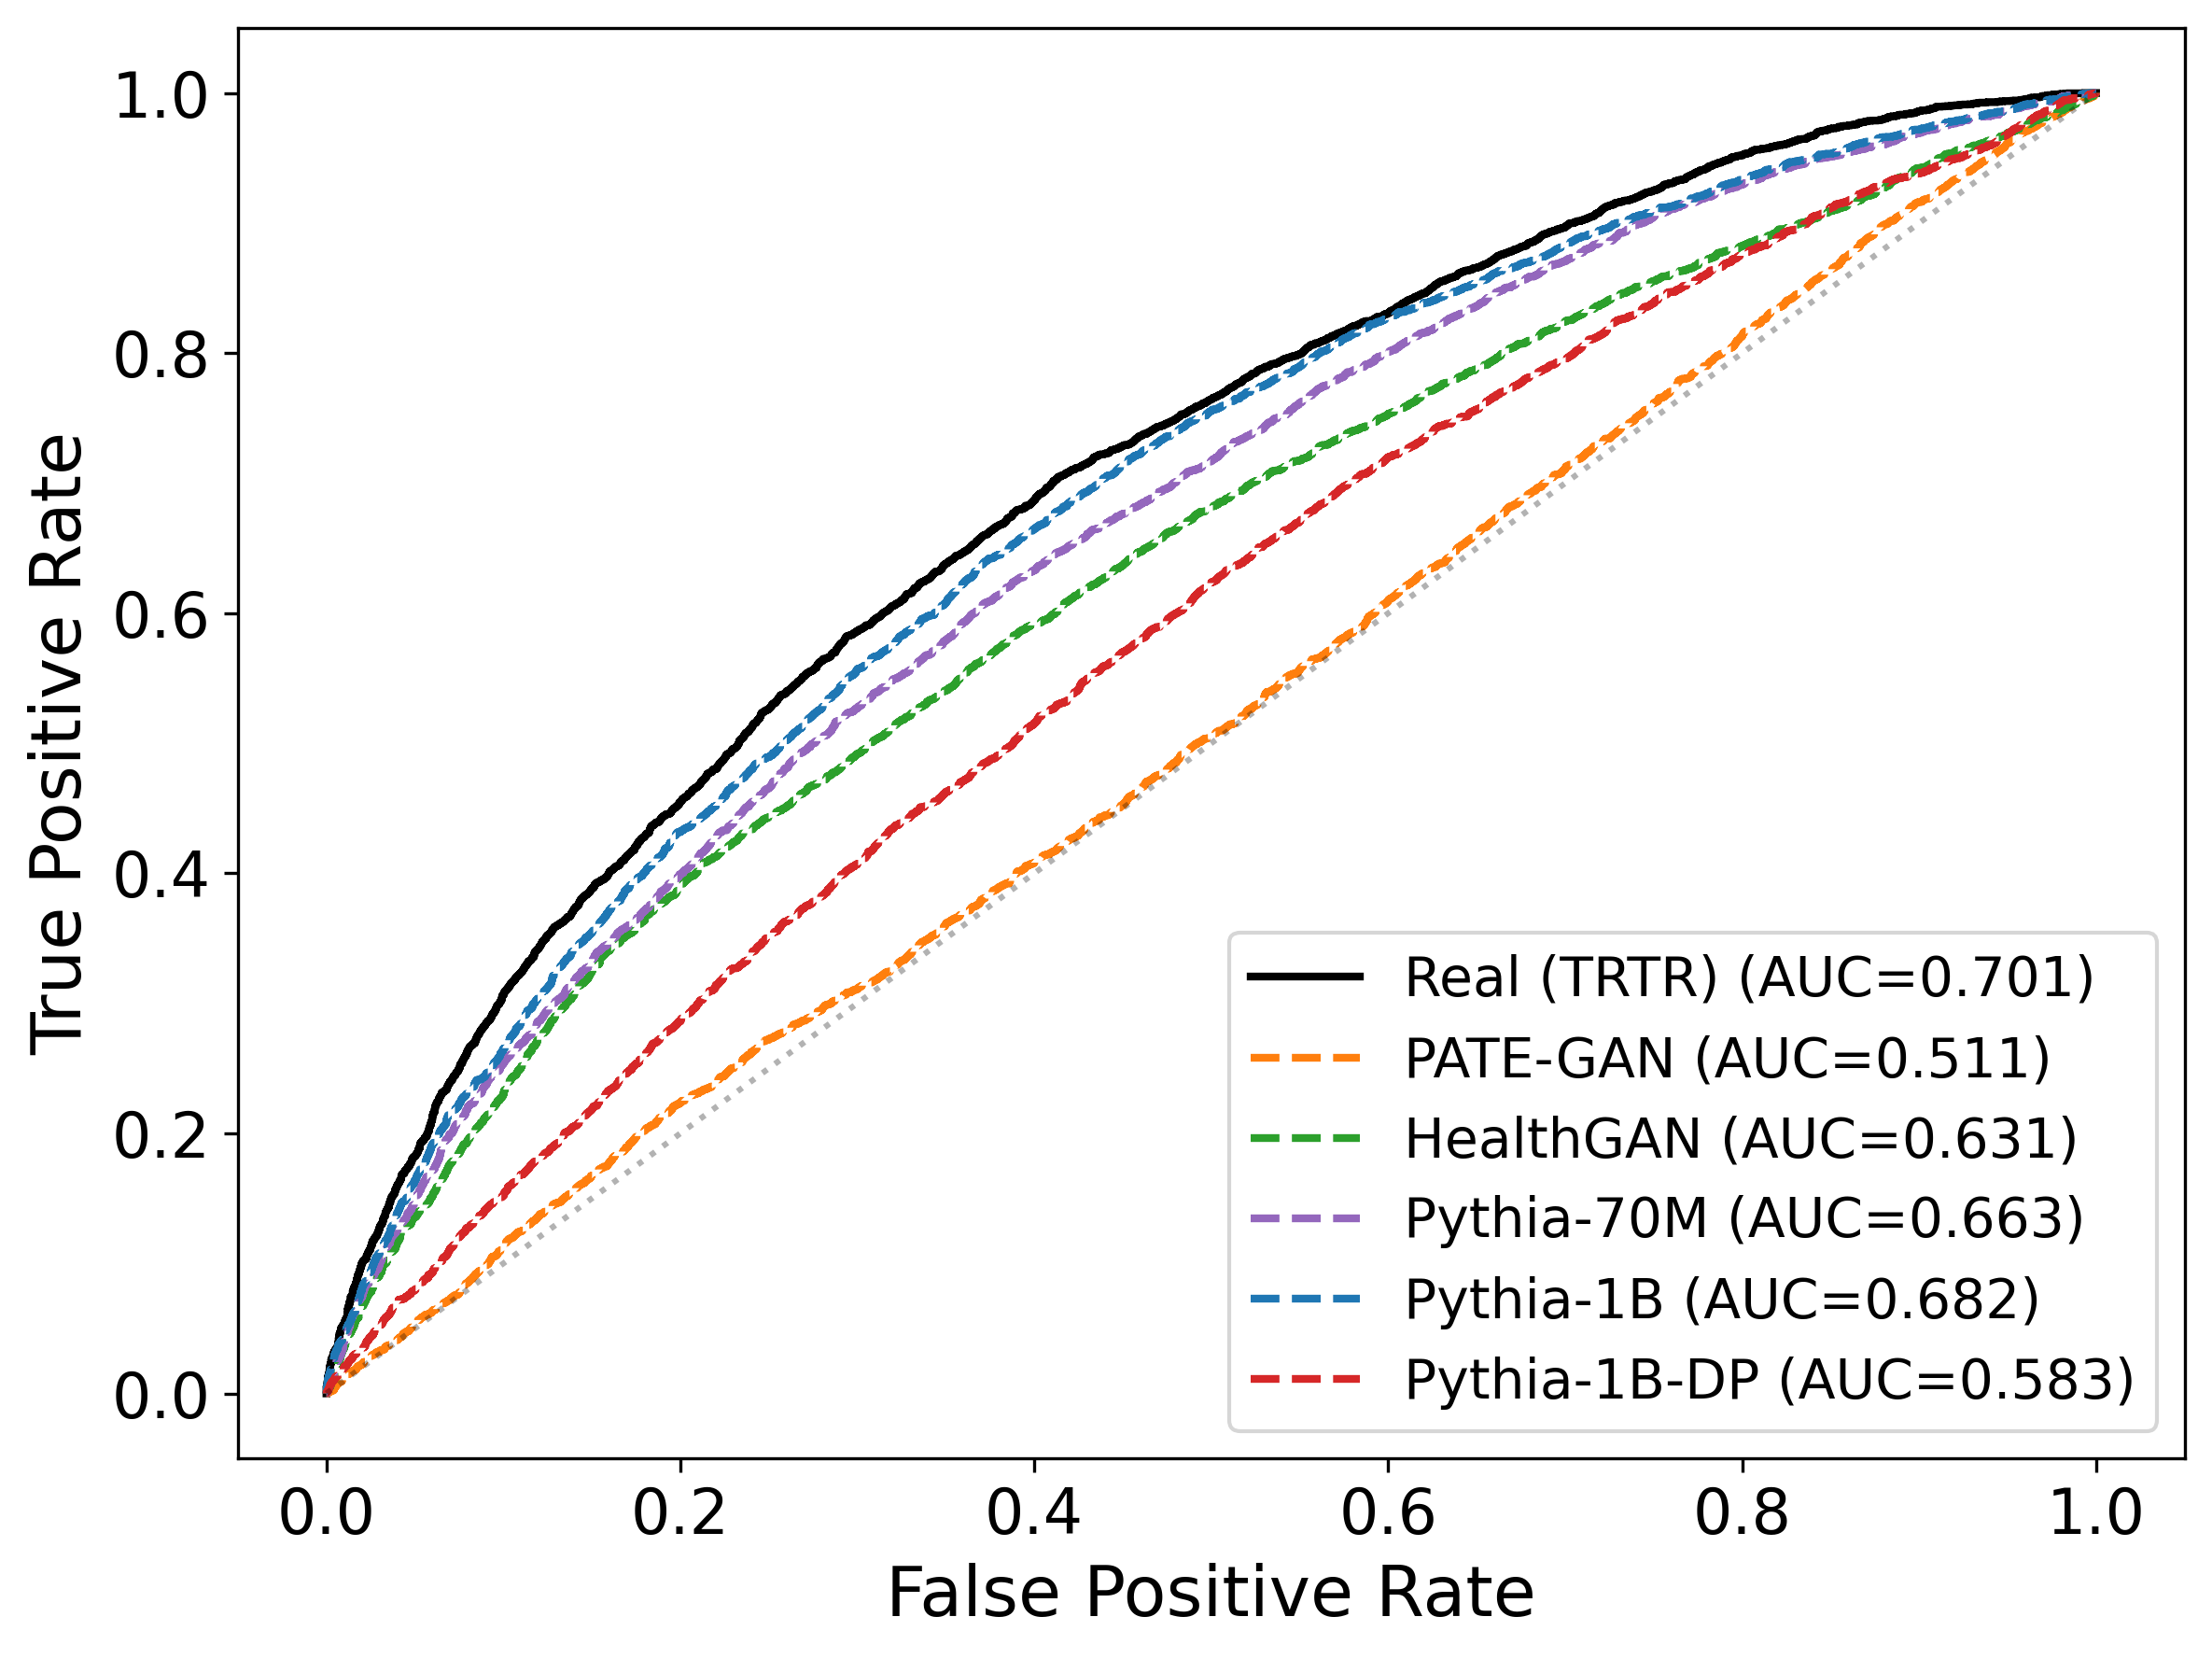
\includegraphics[width=0.75\textwidth]{images/results/2b-roc_curves}
\caption{Gradient-Boosting ROC curves under TSTR for all five generators
and the real (TRTR) reference. Legend values are the corresponding
AUC-ROC scores.}
\label{fig:rq2:roc}
\end{figure}

\paragraph{Feature-Importance Stability:}
Figure~\ref{fig:rq2:featimp} reports the feature-importance agreement
score defined in Section~\ref{sec:eval:utility:predictive:fi}. The score
compares the normalised random-forest importance vector obtained from each
synthetic-trained model with the real-trained reference. Here, 
higher values indicate a more similar distribution of importance
across the engineered features. HealthGAN ($0.914$), Pythia-1B ($0.911$), Pythia-70M ($0.889$),
and Pythia-1B-DP ($0.856$) remain close to the real reference, whereas
PATE-GAN is lower ($0.675$). This suggests that the four non-PATE
generators retain a broadly similar model-based importance profile, while
PATE-GAN departs more strongly. This diagnostic assesses model-specific 
predictive patterns, not as evidence that the
identified predictors are causal or clinically validated. The corresponding
top-ranked features and the PATE-GAN-specific divergence pattern are shown
in Appendix~\ref{app:feature-importance}.

\begin{figure}[!htbp]
\centering
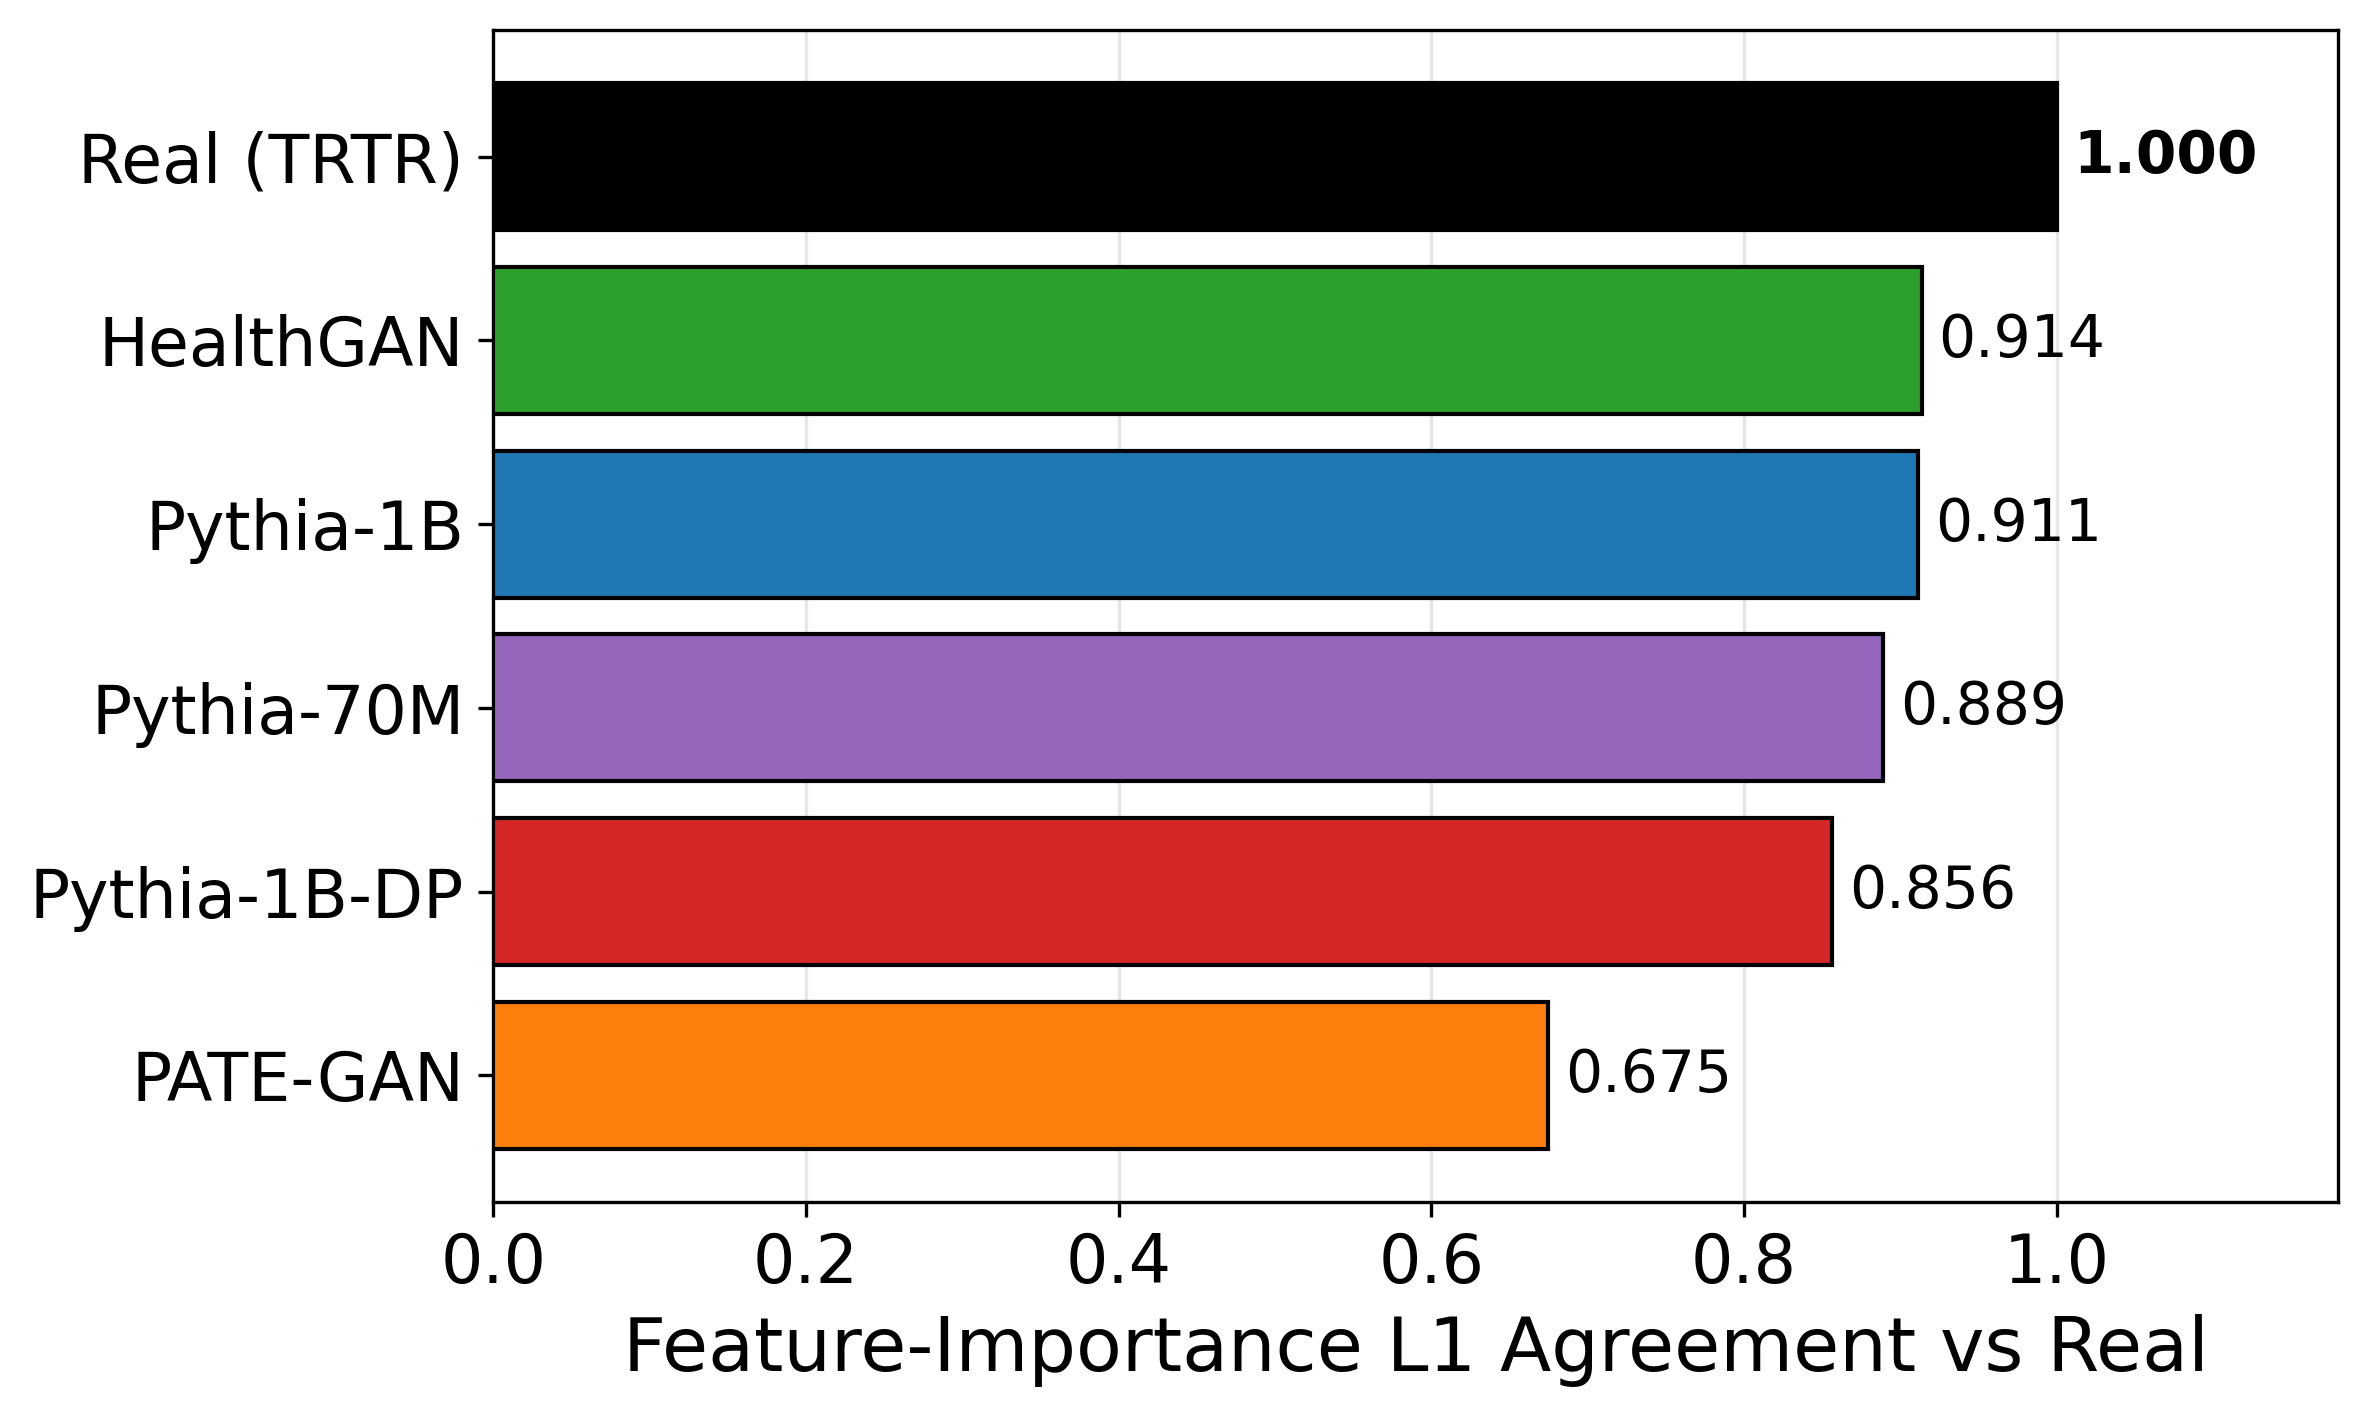
\includegraphics[width=0.76\textwidth]{images/results/2c_ii-feature_importance_l1}
\caption{Feature-importance agreement with the real-trained random-forest
reference. Scores are based on the $L_1$ distance between normalised
importance vectors; higher values indicate closer agreement.}
\label{fig:rq2:featimp}
\end{figure}

\paragraph{Cox Proportional-Hazards Agreement:}
Agreement on a Cox proportional-hazards model
(Section~\ref{sec:eval:utility:predictive:cox}) tests whether the
synthetic data preserve survival-style association patterns. A Cox model is
fitted on each data source. Agreement is
measured by counting the covariates whose synthetic $95\%$ hazard-ratio
confidence intervals overlap the corresponding real-data intervals.
(Section~\ref{sec:eval:utility:predictive:cox-overlap}). The overlap
summary in Table~\ref{tab:rq2:cox} is used as the main result because it is
the scalar Cox metric defined in the methodology. The full per-covariate
hazard-ratio plots are provided in Appendix~\ref{app:cox}.

HealthGAN and the two 1B-parameter Pythia variants show the strongest
agreement on this metric, with seven overlapping covariates each
(HealthGAN: $7/12$; Pythia-1B and Pythia-1B-DP: $7/13$). 
HealthGAN is evaluated on twelve covariates because
\emph{number\_emergency} has zero variance in its synthetic data and was
therefore excluded from the Cox model. Pythia-70M
overlaps on four of thirteen covariates, while PATE-GAN overlaps on none.
The identical overlap counts for Pythia-1B and Pythia-1B-DP indicate that
the utility loss observed under TSTR AUC-ROC is not mirrored by this
coarser Cox-overlap diagnostic. PATE-GAN's result also aligns with our finding 
of distorted dataset generation in this evaluation as well.
This should be read as agreement in fitted
Cox effect-size intervals, not as evidence that the synthetic data validate
clinical causal relationships.

\begin{table}[H]
\centering
\small
\caption{Cox proportional-hazards confidence-interval overlap per
generator: the number of covariates whose synthetic $95\%$ hazard-ratio
interval overlaps the real interval, out of those fitted (higher is
better). HealthGAN is fitted on twelve covariates because one
zero-variance column was dropped.}
\label{tab:rq2:cox}
% Auto-generated by data_analysis.ipynb (2e). Do not edit by hand.
% Requires booktabs.
\begin{tabular}{lcc}
\toprule
Generator & CIs overlapping & Fraction $\uparrow$ \\
\midrule
PATE-GAN & 0 / 13 & 0.000 \\
HealthGAN & 7 / 12 & 0.583 \\
Pythia-70M & 4 / 13 & 0.308 \\
Pythia-1B & 7 / 13 & 0.538 \\
Pythia-1B-DP & 7 / 13 & 0.538 \\
\bottomrule
\end{tabular}

\end{table}

\subsubsection{Ablation: Age Binning Granularity}
\label{sec:results:rq2:utility:age-binning}

The preprocessing pipeline (Section~\ref{sec:data:fe:age}) retains the
dataset's original ten age categories. An earlier approach that grouped
age into three broader categories (young, middle-aged, and elderly) was
not used. Table~\ref{tab:age-binning-tstr} quantifies the impact on
Train-on-Synthetic, Test-on-Real (TSTR) utility for the three generators
with matched runs under both age encodings: PATE-GAN, HealthGAN, and
Pythia-70M. The ablation is therefore a preprocessing-sensitivity check,
not a full five-generator comparison. Pythia-1B and Pythia-1B-DP are not
included because they were introduced after the preprocessing pipeline had
already been revised to the retained ten-bin age encoding. No matched
three-bin runs are available for those models. All evaluations use the
real held-out test split ($n = 14{,}304$) with \emph{readmitted} as the
binary target. Gradient Boosting is used as the primary downstream classifier.
Logistic Regression and Random Forest show similar overall patterns.
\vspace{0.5em}

\begin{table}[H]
\centering
\small
\caption{TSTR utility under the discarded three-bin age encoding versus
the retained ten-bin encoding. Test set: real held-out split
($n = 14{,}304$); target: \emph{readmitted}; classifier: Gradient
Boosting. $\Delta$ is computed as the difference from 10-bin value to the 3-bin
value.}
\label{tab:age-binning-tstr}
\begin{tabular}{llccc}
\toprule
Train Source & Metric & 3-bin & 10-bin & $\Delta$ \\
\midrule
Real (TRTR) & AUC-ROC & 0.7014 & 0.7008 & $-0.0006$ \\
Real (TRTR) & F1      & 0.3644 & 0.3668 & $+0.0024$ \\
\midrule
PATE-GAN    & AUC-ROC & 0.4823 & 0.5108 & $+0.0285$ \\
PATE-GAN    & F1      & 0.0437 & 0.0093 & $-0.0344$ \\
HealthGAN   & AUC-ROC & 0.6605 & 0.6312 & $-0.0293$ \\
HealthGAN   & F1      & 0.2647 & 0.3824 & $+0.1177$ \\
Pythia-70M  & AUC-ROC & 0.5981 & \textbf{0.6634} & $\mathbf{+0.0653}$ \\
Pythia-70M  & F1      & 0.3944 & \textbf{0.5005} & $\mathbf{+0.1061}$ \\
\bottomrule
\end{tabular}
\end{table}

The Train-on-Real Test-on-Real is essentially unchanged between the two
encodings, indicating that the ablation does not alter the real-data
prediction task in a meaningful way. Within the matched generators,
however, the effect is model-dependent. Pythia-70M improves most under
the retained ten-bin encoding (AUC-ROC $+0.0653$; F1 $+0.1061$),
suggesting that the token-based generator benefited from the more detailed
age representation. HealthGAN shows a mixed response: AUC-ROC is higher
under the discarded three-bin encoding, whereas F1 is higher under the
retained ten-bin encoding. PATE-GAN remains weak under both settings, so
age granularity is unlikely to be its primary utility bottleneck in this
experiment. Overall, the ablation supports the ten-bin preprocessing
choice while showing that age encoding can affect generators differently.

% ROC, feature-importance, and Cox predictive results are reported above
% within Predictive Performance (§\ref{sec:results:rq2:utility:predictive});
% the age-binning ablation is a preprocessing-sensitivity finding kept as
% the final subsubsection of the utility results.

\subsection{Privacy Results}
\label{sec:results:rq2:privacy}

Privacy is assessed using the empirical metrics defined in
Section~\ref{sec:eval:privacy}. These include distance-based proximity
measures, outlier-linkability analysis, and inference-attack
simulations. Each metric examines a specific disclosure risk and does
not independently provide a formal privacy guarantee. The privacy
results are therefore interpreted together and alongside the utility
results, since synthetic data that depart substantially from the real
distribution may appear private under distance-based measures. Selected
privacy diagnostics are summarised in Figure~\ref{fig:rq2:privacy}.

\paragraph{Nearest-Neighbour Distance and Distance Ratio:}
Table~\ref{tab:rq2:nn} presents the median and fifth-percentile
nearest-neighbour distances in both directions for each generator. It
also reports the NNDR defined in
Section~\ref{sec:eval:privacy:nn}. The median represents typical record
proximity. In the synthetic-to-real direction, the fifth percentile
focuses on the lower tail of records closest to the real data and is
therefore more relevant to disclosure risk. An NNDR close to one
indicates that synthetic-to-real proximity is similar to the spacing
between real records. It is important to note that, NNDR is a proximity diagnostic and does
not independently demonstrate privacy.

\begin{table}[H]
\centering
\small
\caption{Median and fifth-percentile nearest-neighbour distances and
median NNDR for each generator. The fifth-percentile synthetic-to-real
distance describes the lower proximity tail. The median real-to-real
nearest-neighbour distance is $2.019$ and is included as a descriptive
reference. Larger synthetic-to-real distances and
$\text{NNDR} \geq 1$ suggest lower proximity risk only when the
synthetic data also preserve the real-data distribution.}
\label{tab:rq2:nn}
% Auto-generated by data_analysis.ipynb (3a). Do not edit by hand.
% Requires booktabs.
\begin{tabular}{lccccc}
\toprule
 & R$\rightarrow$S median & R$\rightarrow$S 5th pct & S$\rightarrow$R median & S$\rightarrow$R 5th pct & NNDR median \\
\midrule
PATE-GAN & 41.268 & 39.706 & 219.879 & 79.995 & 104.601 \\
HealthGAN & 2.924 & 1.439 & 2.233 & 1.136 & 1.063 \\
Pythia-70M & 2.684 & 1.140 & 1.440 & 0.771 & 0.721 \\
Pythia-1B & 2.581 & 1.060 & 1.406 & 0.727 & 0.698 \\
Pythia-1B-DP & 2.811 & 1.217 & 1.533 & 0.833 & 0.763 \\
\bottomrule
\end{tabular}

\end{table}

The four non-PATE generators produce synthetic records at distances
comparable to the typical spacing between real records. HealthGAN has
a median synthetic-to-real distance of $2.233$ and an NNDR of $1.063$,
both close to the real-to-real reference. The three Pythia variants
have lower median distances of $1.406$-$1.533$ and NNDR values of
$0.698$-$0.763$. This indicates that their synthetic records are
typically closer to the real data than real records are to one another.
However, this proximity alone does not justify that records were
copied.

PATE-GAN produces a much larger median synthetic-to-real distance of
$219.879$ and an NNDR of $104.601$. Given its poor similarity results
in Section~\ref{sec:results:rq2:utility:similarity}, these values indicate
that its records have moved away from the real-data distribution. They
should therefore be interpreted as poor fidelity rather than strong
privacy protection. This result demonstrates why distance-based privacy
metrics must be considered together with utility and fidelity measures.

For the four non-PATE generators, the fifth-percentile
synthetic-to-real distances range from $0.727$ to $1.136$. These
positive values indicate that the lower proximity tail generally
remains separated from the real data. However, a positive fifth
percentile cannot exclude rarer exact or near-exact matches below that
percentile. Together with the NNAA and membership-inference results in
Sections~\ref{sec:results:rq2:privacy:nnaa}
and~\ref{sec:results:rq2:privacy:mia}, the findings provide no evidence
of widespread training-record memorisation. PATE-GAN's
fifth-percentile distance of $79.995$ reflects the same distributional
drift as its median and should not be interpreted as evidence of
effective privacy protection.

\paragraph{Nearest-Neighbour Adversarial Accuracy:}
\label{sec:results:rq2:privacy:nnaa}

Nearest-neighbour adversarial accuracy (NNAA) in
Section~\ref{sec:eval:privacy:nnaa} is calculated separately for the
training and test sets. The ideal value for both TrainAA and TestAA is
$0.5$, indicating that the adversary performs no better than random
guessing when distinguishing synthetic from real records. Privacy loss is
calculated as the difference between TestAA and TrainAA, with a value near
zero indicating little evidence of training-set memorisation.
Table~\ref{tab:rq2:nnaa} reports these three values.

\begin{table}[H]
\centering
\small
\caption{Nearest-neighbour adversarial accuracy per generator. Train and
test adversarial accuracy near $0.5$ indicates good resemblance. Privacy
loss (test $-$ train) near $0.0$ indicates no memorisation.}
\label{tab:rq2:nnaa}
% Auto-generated by data_analysis.ipynb (3a_ii). Do not edit by hand.
% Requires booktabs.
\begin{tabular}{lccc}
\toprule
Generator & Train AA & Test AA & Privacy loss \\
\midrule
PATE-GAN & 1.0000 & 0.9999 & $-0.0001$ \\
HealthGAN & 0.7182 & 0.7199 & $+0.0017$ \\
Pythia-70M & 0.6469 & 0.6499 & $+0.0030$ \\
Pythia-1B & 0.6207 & 0.6204 & $-0.0003$ \\
Pythia-1B-DP & 0.7063 & 0.7139 & $+0.0076$ \\
\bottomrule
\end{tabular}

\end{table}

Privacy loss is close to zero for all generators, ranging from $-0.0001$
to $+0.0076$. This provides no meaningful evidence that the generators
reproduce training records more closely than held-out records. PATE-GAN's
NNAA of approximately $1.0$ shows that its synthetic data are easily
distinguishable from the real data, whereas the other generators achieve
values between $0.62$ and $0.72$. Pythia-1B is closest to the ideal value
of $0.5$ ($0.621$), although all generators remain distinguishable from
the real data. Overall, the near-zero privacy loss suggests that this
distinguishability is not caused by training-set memorisation.

\paragraph{Membership Inference:}
\label{sec:results:rq2:privacy:mia}

A distance-based membership-inference adversary
(Section~\ref{sec:eval:privacy:mia}) attempts to decide whether a given
real record was part of the generator's training set.
Table~\ref{tab:rq2:mia} reports the AUC-ROC achieved by the membership-inference attack.

\begin{table}[H]
\centering
\small
\caption{Membership-inference attack results per generator. AUC near
$0.5$ and advantage near $0.0$ indicate that the adversary cannot
distinguish training members from non-members.}
\label{tab:rq2:mia}
% Auto-generated by data_analysis.ipynb (3b). Do not edit by hand.
% Requires booktabs.
\begin{tabular}{lcc}
\toprule
Generator & MIA AUC & MIA advantage \\
\midrule
PATE-GAN & 0.4984 & $-0.0016$ \\
HealthGAN & 0.5005 & $+0.0005$ \\
Pythia-70M & 0.5119 & $+0.0119$ \\
Pythia-1B & 0.4926 & $-0.0074$ \\
Pythia-1B-DP & 0.4931 & $-0.0069$ \\
\bottomrule
\end{tabular}

\end{table}

Membership-inference performance remains close to random guessing across
all generators. Every attack AUC lies within $[0.493, 0.512]$ of the
random-guess baseline, and every advantage is within $\pm 0.012$ of zero.
The largest signal, Pythia-70M's AUC of
$0.512$, remains negligible. No generator, private or otherwise, shows
evidence of exploitable membership leakage under this distance-based
adversary. This is consistent with the absence of memorisation indicated
by the privacy-loss measure above.

\paragraph{Attribute Inference:}
\label{sec:results:rq2:privacy:aia}

The attribute-inference attack
(Section~\ref{sec:eval:privacy:aia}) evaluates whether a predictor trained
on synthetic data can recover sensitive attributes from real records more
accurately than a marginal baseline. Table~\ref{tab:rq2:aia} reports 
the per-attribute advantage for
the four attributes considered. The final column reports the 
maximum advantage for each generator and is
used in the comprehensive summary.

\begin{table}[H]
\centering
\small
\caption{Attribute-inference advantage per generator and attribute
(positive values indicate leakage above the marginal baseline). The
final column is the per-generator maximum advantage.}
\label{tab:rq2:aia}
% Auto-generated by data_analysis.ipynb (3c). Do not edit by hand.
% Requires booktabs.
\begin{tabular}{lccccc}
\toprule
Generator & \texttt{readmitted} & \texttt{gender} & \texttt{age} & \texttt{diag\_1} & Max \\
\midrule
PATE-GAN & $-0.3334$ & $-0.0560$ & $-0.0266$ & $-0.2330$ & $-0.0266$ \\
HealthGAN & $-0.0046$ & $-0.0040$ & $-0.0338$ & $-0.0218$ & $-0.0040$ \\
Pythia-70M & $-0.0236$ & $-0.0052$ & $-0.0332$ & $+0.0064$ & $+0.0064$ \\
Pythia-1B & $-0.0168$ & $+0.0104$ & $+0.0024$ & $+0.0410$ & $+0.0410$ \\
Pythia-1B-DP & $-0.0296$ & $-0.0056$ & $-0.0322$ & $-0.0166$ & $-0.0056$ \\
\bottomrule
\end{tabular}

\end{table}

Most advantage values are zero or negative, indicating that the attack
does not outperform the marginal baseline. Pythia-1B is the main
exception, showing a small positive advantage for the primary diagnosis
(\emph{diag\_1}, $+0.0410$) and smaller advantages for \emph{gender} and
\emph{age}. This signal is absent in Pythia-1B-DP, whose \emph{diag\_1}
advantage is $-0.0166$ and maximum advantage is $-0.0056$. This represents
the main privacy improvement of differential privacy within the LLM
family and is examined further in
Section~\ref{sec:results:rq3:llm-toggle}. PATE-GAN's strongly negative
values for \emph{readmitted} ($-0.3334$) and \emph{diag\_1} ($-0.2330$)
reflect its limited data quality rather than stronger privacy protection.

\paragraph{Outlier Linkability:}
\label{sec:results:rq2:privacy:linkability}

The clustering-proximity test
(Section~\ref{sec:eval:privacy:linkability}) evaluates disclosure risk
for unusual real records. It compares the percentage of outliers and
non-outliers that have a nearby synthetic record within a radius of
$2.636$, corresponding to the $75^{\text{th}}$ percentile of real-to-real
nearest-neighbour distances. The $5\%$ of real records farthest from the
data centroid ($2{,}861$ records) are defined as outliers.
Table~\ref{tab:rq2:linkability} reports both percentages and their
difference.

\begin{table}[H]
\centering
\small
\caption{Outlier versus non-outlier linkability per generator (percentage
of real records with a synthetic neighbour within radius $2.636$). Low
outlier linkability indicates that the generator does not concentrate mass
around vulnerable records; a positive gap indicates coverage of common
rather than extreme patterns. The gap is reported in percentage points.}
\label{tab:rq2:linkability}
% Auto-generated by data_analysis.ipynb (3d). Do not edit by hand.
% Requires booktabs.
\begin{tabular}{lccc}
\toprule
Generator & Outlier \% & Non-outlier \% & Gap (pp) \\
\midrule
PATE-GAN & 0.0 & 0.0 & $+0.0$ \\
HealthGAN & 0.0 & 42.0 & $+42.0$ \\
Pythia-70M & 0.1 & 50.6 & $+50.6$ \\
Pythia-1B & 0.6 & 53.3 & $+52.6$ \\
Pythia-1B-DP & 0.0 & 46.8 & $+46.8$ \\
\bottomrule
\end{tabular}

\end{table}

Outlier linkability is near zero for every generator (at most $0.6\%$, for
Pythia-1B), indicating that very few vulnerable tail records have a nearby
synthetic neighbour. The non-collapsed generators link a substantial
fraction of non-outliers ($42$-$53\%$). The resulting large positive
gap is consistent with the intended pattern. Common clinical regions are
covered while rare, identifiable records remain largely uncovered.
PATE-GAN links neither outliers nor non-outliers
($0\%$ on both), consistent with output that lies away from the real
manifold altogether.

\begin{figure}[H]
\centering
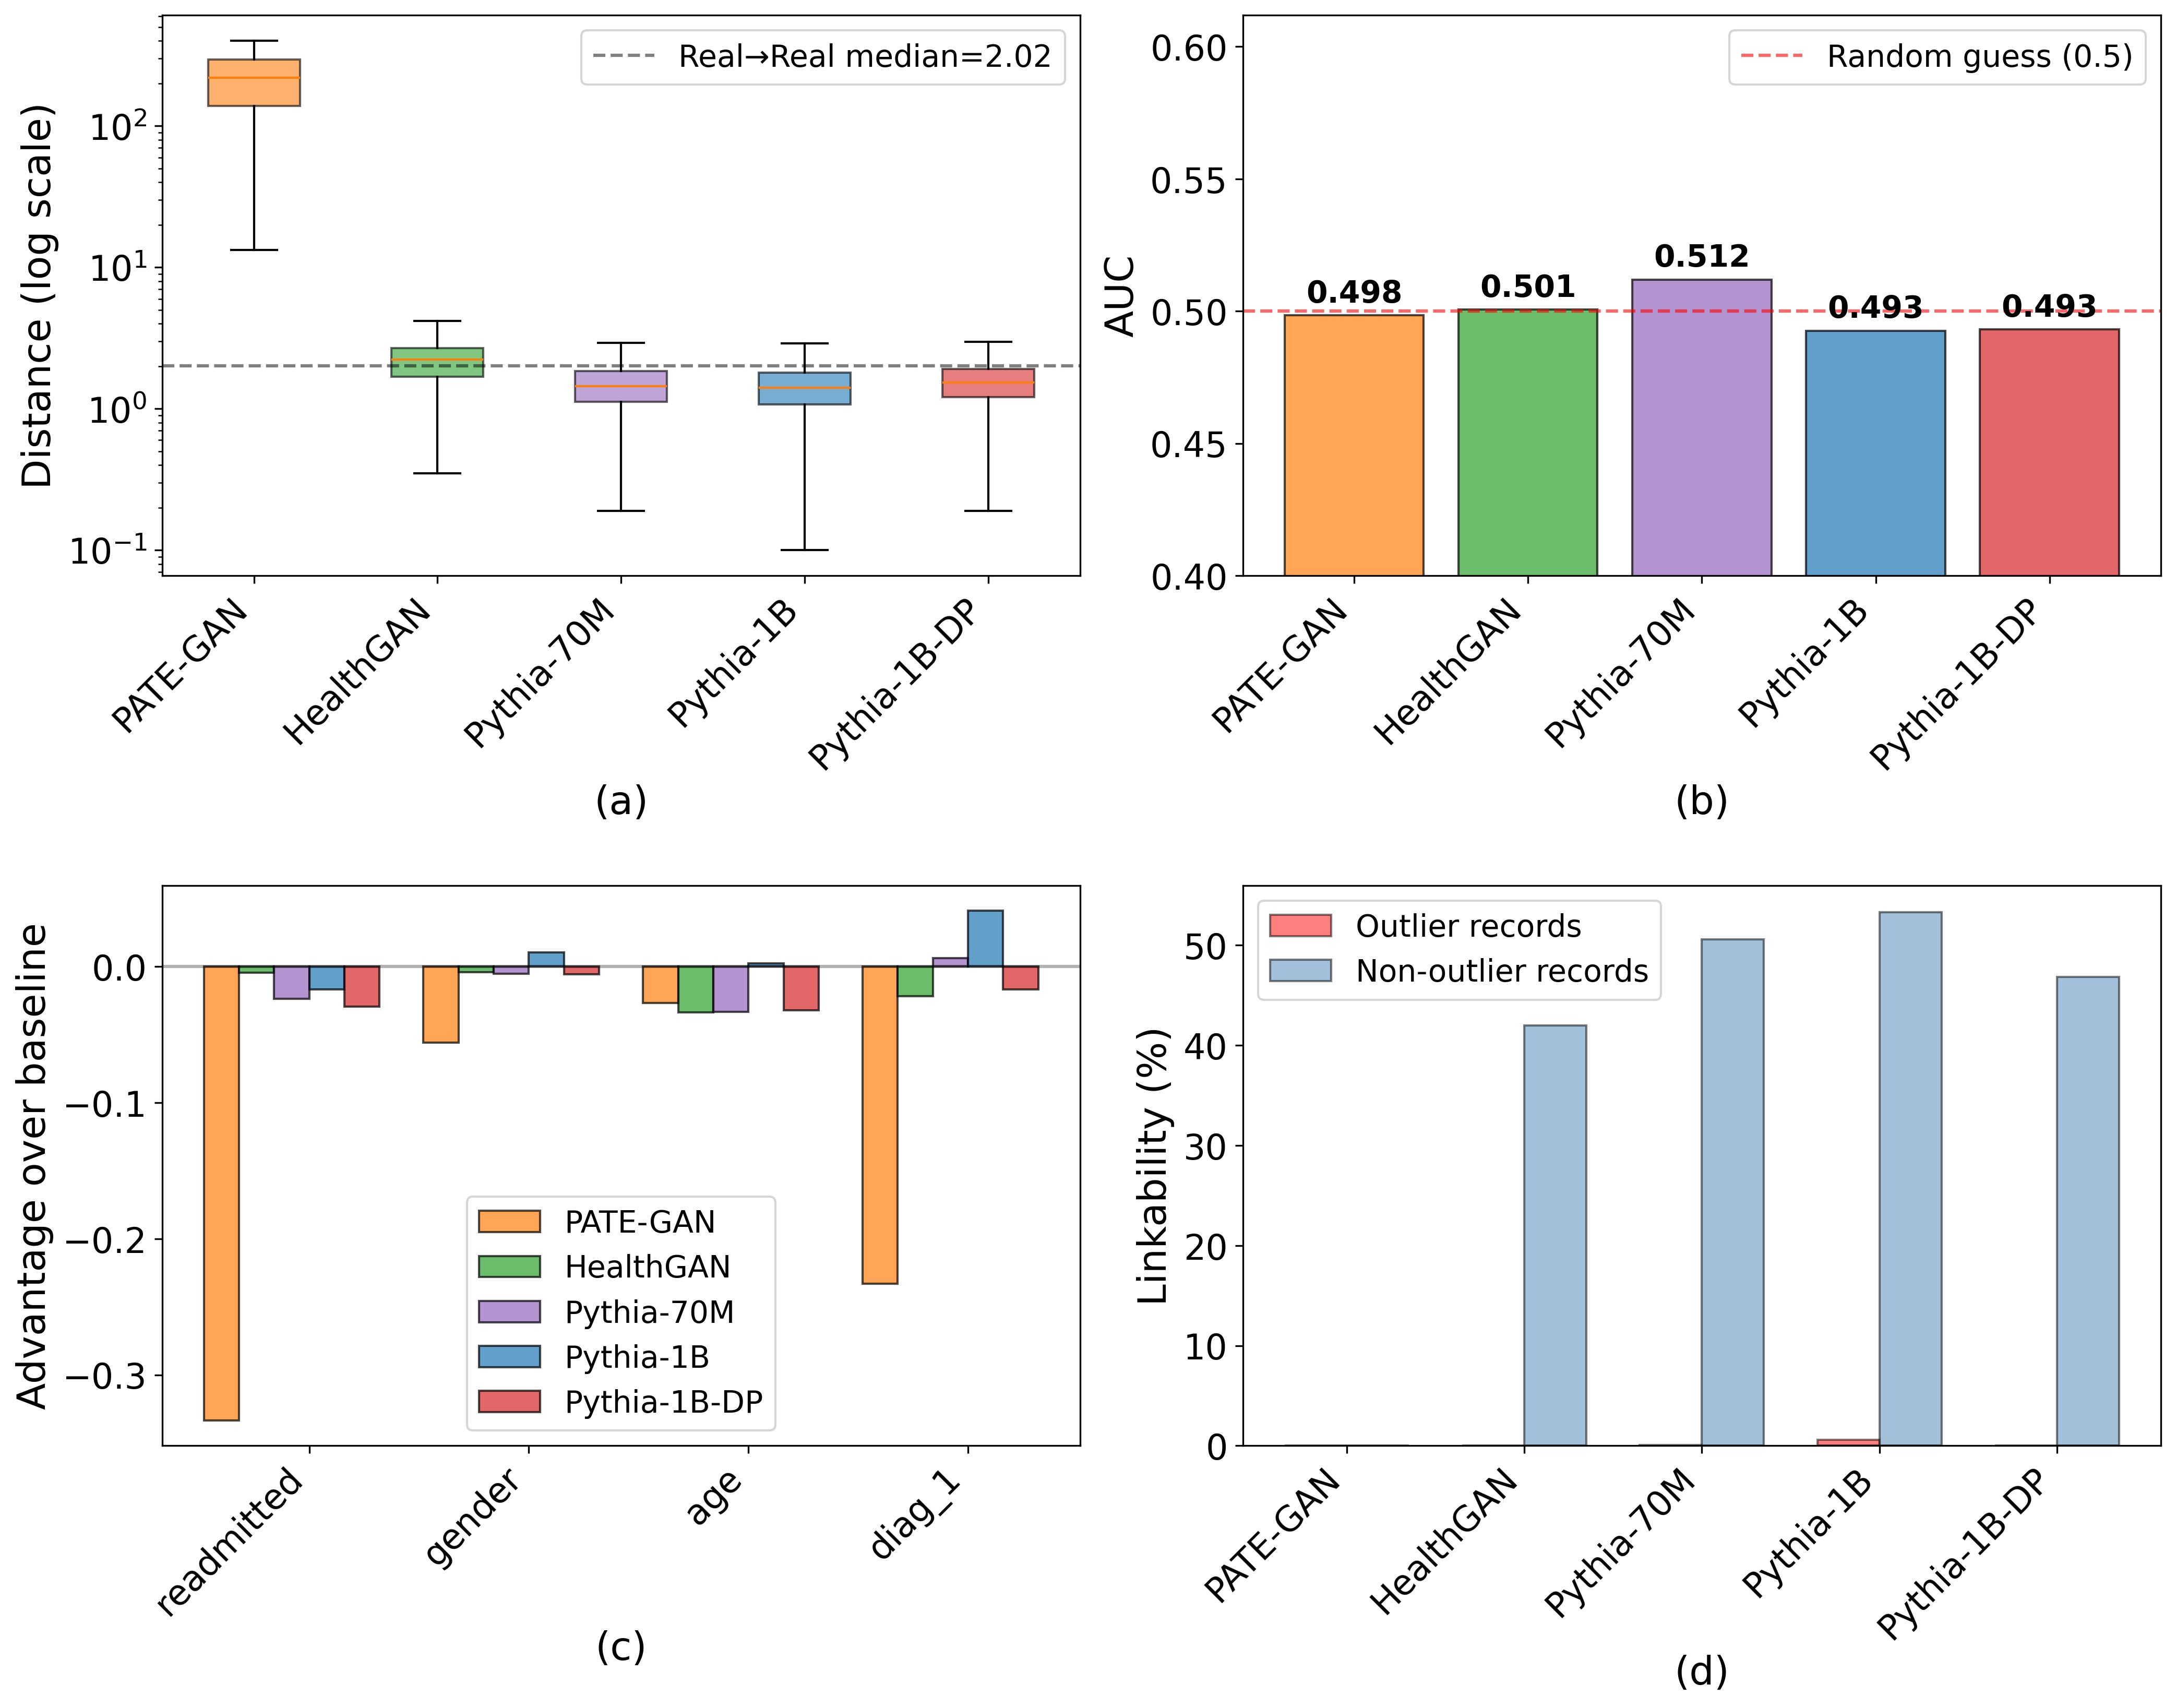
\includegraphics[width=\textwidth]{images/results/3e-privacy_evaluation}
\caption{Consolidated privacy diagnostics across the five generators:
(a)~synthetic-to-real nearest-neighbour distance on a log scale,
(b)~membership-inference AUC
against the random-guess baseline, (c)~attribute-inference
advantage per attribute, and (d)~outlier versus non-outlier
linkability.}
\label{fig:rq2:privacy}
\end{figure}

\subsection{Comparative Aggregation Results}
\label{sec:results:rq2:aggregation}

The per-metric utility and privacy results of the two preceding
subsections are now combined into the small set of aggregation views
introduced in Section~\ref{sec:eval:aggregate}. These views are
interpretive rather than decisive. The comparative claims remain grounded
in the raw metric values, and the presentation proceeds from the unscaled
summary table to the scaled visual displays. The comprehensive table is
therefore given first as the numerical reference, followed by the
privacy-utility landscape, the utility radar, the utility-privacy
heatmap, and finally the Pareto analysis that addresses the balance
question of RQ2.

\paragraph{Comprehensive Summary:}
\label{sec:results:rq2:table}

Table~\ref{tab:rq2:summary} collects the twelve headline single-number
metrics for the five generators and the real reference in a single view,
grouped by pillar and branch. It preserves the raw values used for the
main scalar comparison. Feature-importance agreement is reported in the
predictive-utility subsection and included in the utility radar, but is
not repeated here so that the table remains aligned with the twelve
headline rows defined in the methodology. The best value per row among
the synthetic generators is shown in bold for the utility rows. The
privacy rows are left unmarked because PATE-GAN's distance metrics, as
noted, reflect collapse rather than protection.

\begin{table}[H]
\centering
\footnotesize
\setlength{\tabcolsep}{3.5pt}
\caption{Comprehensive summary of the twelve headline metrics across the
five generators and the real (TRTR) reference. Arrows indicate the
preferred direction; ($\approx 0.5$) indicates that values closest to
$0.5$ are best, and ($\approx 0$) indicates negligible leakage.The nearest-neighbour distance and its normalised ratio should be
interpreted relative to the real-data reference values of
$\approx 2.02$ and $\approx 1$, respectively. Lower values indicate
increased proximity risk. Higher values suggest greater separation only
when the synthetic data remain consistent with the real-data
distribution. Otherwise, they may indicate poor fidelity rather than
stronger privacy. Bold marks the best synthetic value on each utility row.
PATE-GAN's nearest-neighbour distance and ratio are not treated as
protective because they reflect off-manifold output and should be read
with Section~\ref{sec:results:rq2:privacy}.}
\label{tab:rq2:summary}
% Auto-generated by data_analysis.ipynb (4c). Do not edit by hand.
% Requires booktabs.
\begin{tabular}{lcccccc}
\toprule
Metric & Real & PATE-GAN & HealthGAN & Pythia-70M & Pythia-1B & Pythia-1B-DP \\
\midrule
\multicolumn{7}{l}{\emph{Statistical similarity}}\\
Mean KS $\downarrow$ & --- & 0.5381 & \textbf{0.0480} & 0.0856 & 0.0805 & 0.0992 \\
Corr.\ diff.\ $\downarrow$ & --- & 0.1142 & 0.0336 & 0.0308 & \textbf{0.0206} & 0.0466 \\
\midrule
\multicolumn{7}{l}{\emph{Predictive utility}}\\
AUC-ROC $\uparrow$ & 0.7008 & 0.5108 & 0.6312 & 0.6634 & \textbf{0.6818} & 0.5827 \\
F1 $\uparrow$ & 0.3668 & 0.0093 & 0.3824 & 0.5005 & \textbf{0.5036} & 0.2714 \\
Cox CI overlap $\uparrow$ & --- & 0.0000 & \textbf{0.5833} & 0.3077 & 0.5385 & 0.5385 \\
\midrule
\multicolumn{7}{l}{\emph{Privacy}}\\
NN dist.\ median $\uparrow$ & --- & 219.879 & 2.233 & 1.440 & 1.406 & 1.533 \\
NNDR median $\uparrow$ & --- & 104.601 & 1.063 & 0.721 & 0.698 & 0.763 \\
MIA AUC ($\approx 0.5$) & --- & 0.4984 & 0.5005 & 0.5119 & 0.4926 & 0.4931 \\
MIA advantage $\downarrow$ & --- & $-0.0016$ & 0.0005 & 0.0119 & $-0.0074$ & $-0.0069$ \\
NNAA priv.\ loss ($\approx 0$) & --- & $-0.0001$ & 0.0017 & 0.0030 & $-0.0003$ & 0.0076 \\
Max.\ attr.\ adv.\ $\downarrow$ & --- & $-0.0266$ & $-0.0040$ & 0.0064 & 0.0410 & $-0.0056$ \\
Outlier link.\ \% $\downarrow$ & --- & 0.0 & 0.0 & 0.1 & 0.6 & 0.0 \\
\bottomrule
\end{tabular}

\end{table}

The table makes the division of strengths explicit. On the utility side,
Pythia-1B is strongest on correlation difference, AUC-ROC, and F1, while
HealthGAN is strongest on mean KS and Cox confidence-interval overlap.
The table therefore separates predictive and joint-structure performance
from marginal and survival-model agreement, rather than identifying one
uniformly superior generator. On the privacy side, membership-inference
AUC, membership-inference advantage, and NNAA privacy loss remain close
to their baseline values for all usable generators. The remaining
separation is metric-specific. HealthGAN is the only usable generator
above the NNDR unity reference line, while Pythia-1B shows the only
positive maximum attribute-inference advantage, a signal that is not
present for Pythia-1B-DP. These differences are revisited in the
within-family DP analysis of Section~\ref{sec:results:rq3}.

\paragraph{Privacy-Utility Landscape:}
\label{sec:results:rq2:landscape}

Figure~\ref{fig:rq2:landscape} positions all five generators on a single
privacy-utility plane, with predictive utility (Gradient-Boosting TSTR
AUC-ROC) on the horizontal axis and a distance-based privacy measure (the
median nearest-neighbour distance ratio) on the vertical axis. The dashed
reference lines mark the real-data utility ceiling (AUC $0.701$) and the
NNDR reference line of unity. This is the primary figure for the first
half of RQ2 where it shows where each family sits on the selected AUC-ROC/NNDR
view.

\begin{figure}[!ht]
\centering
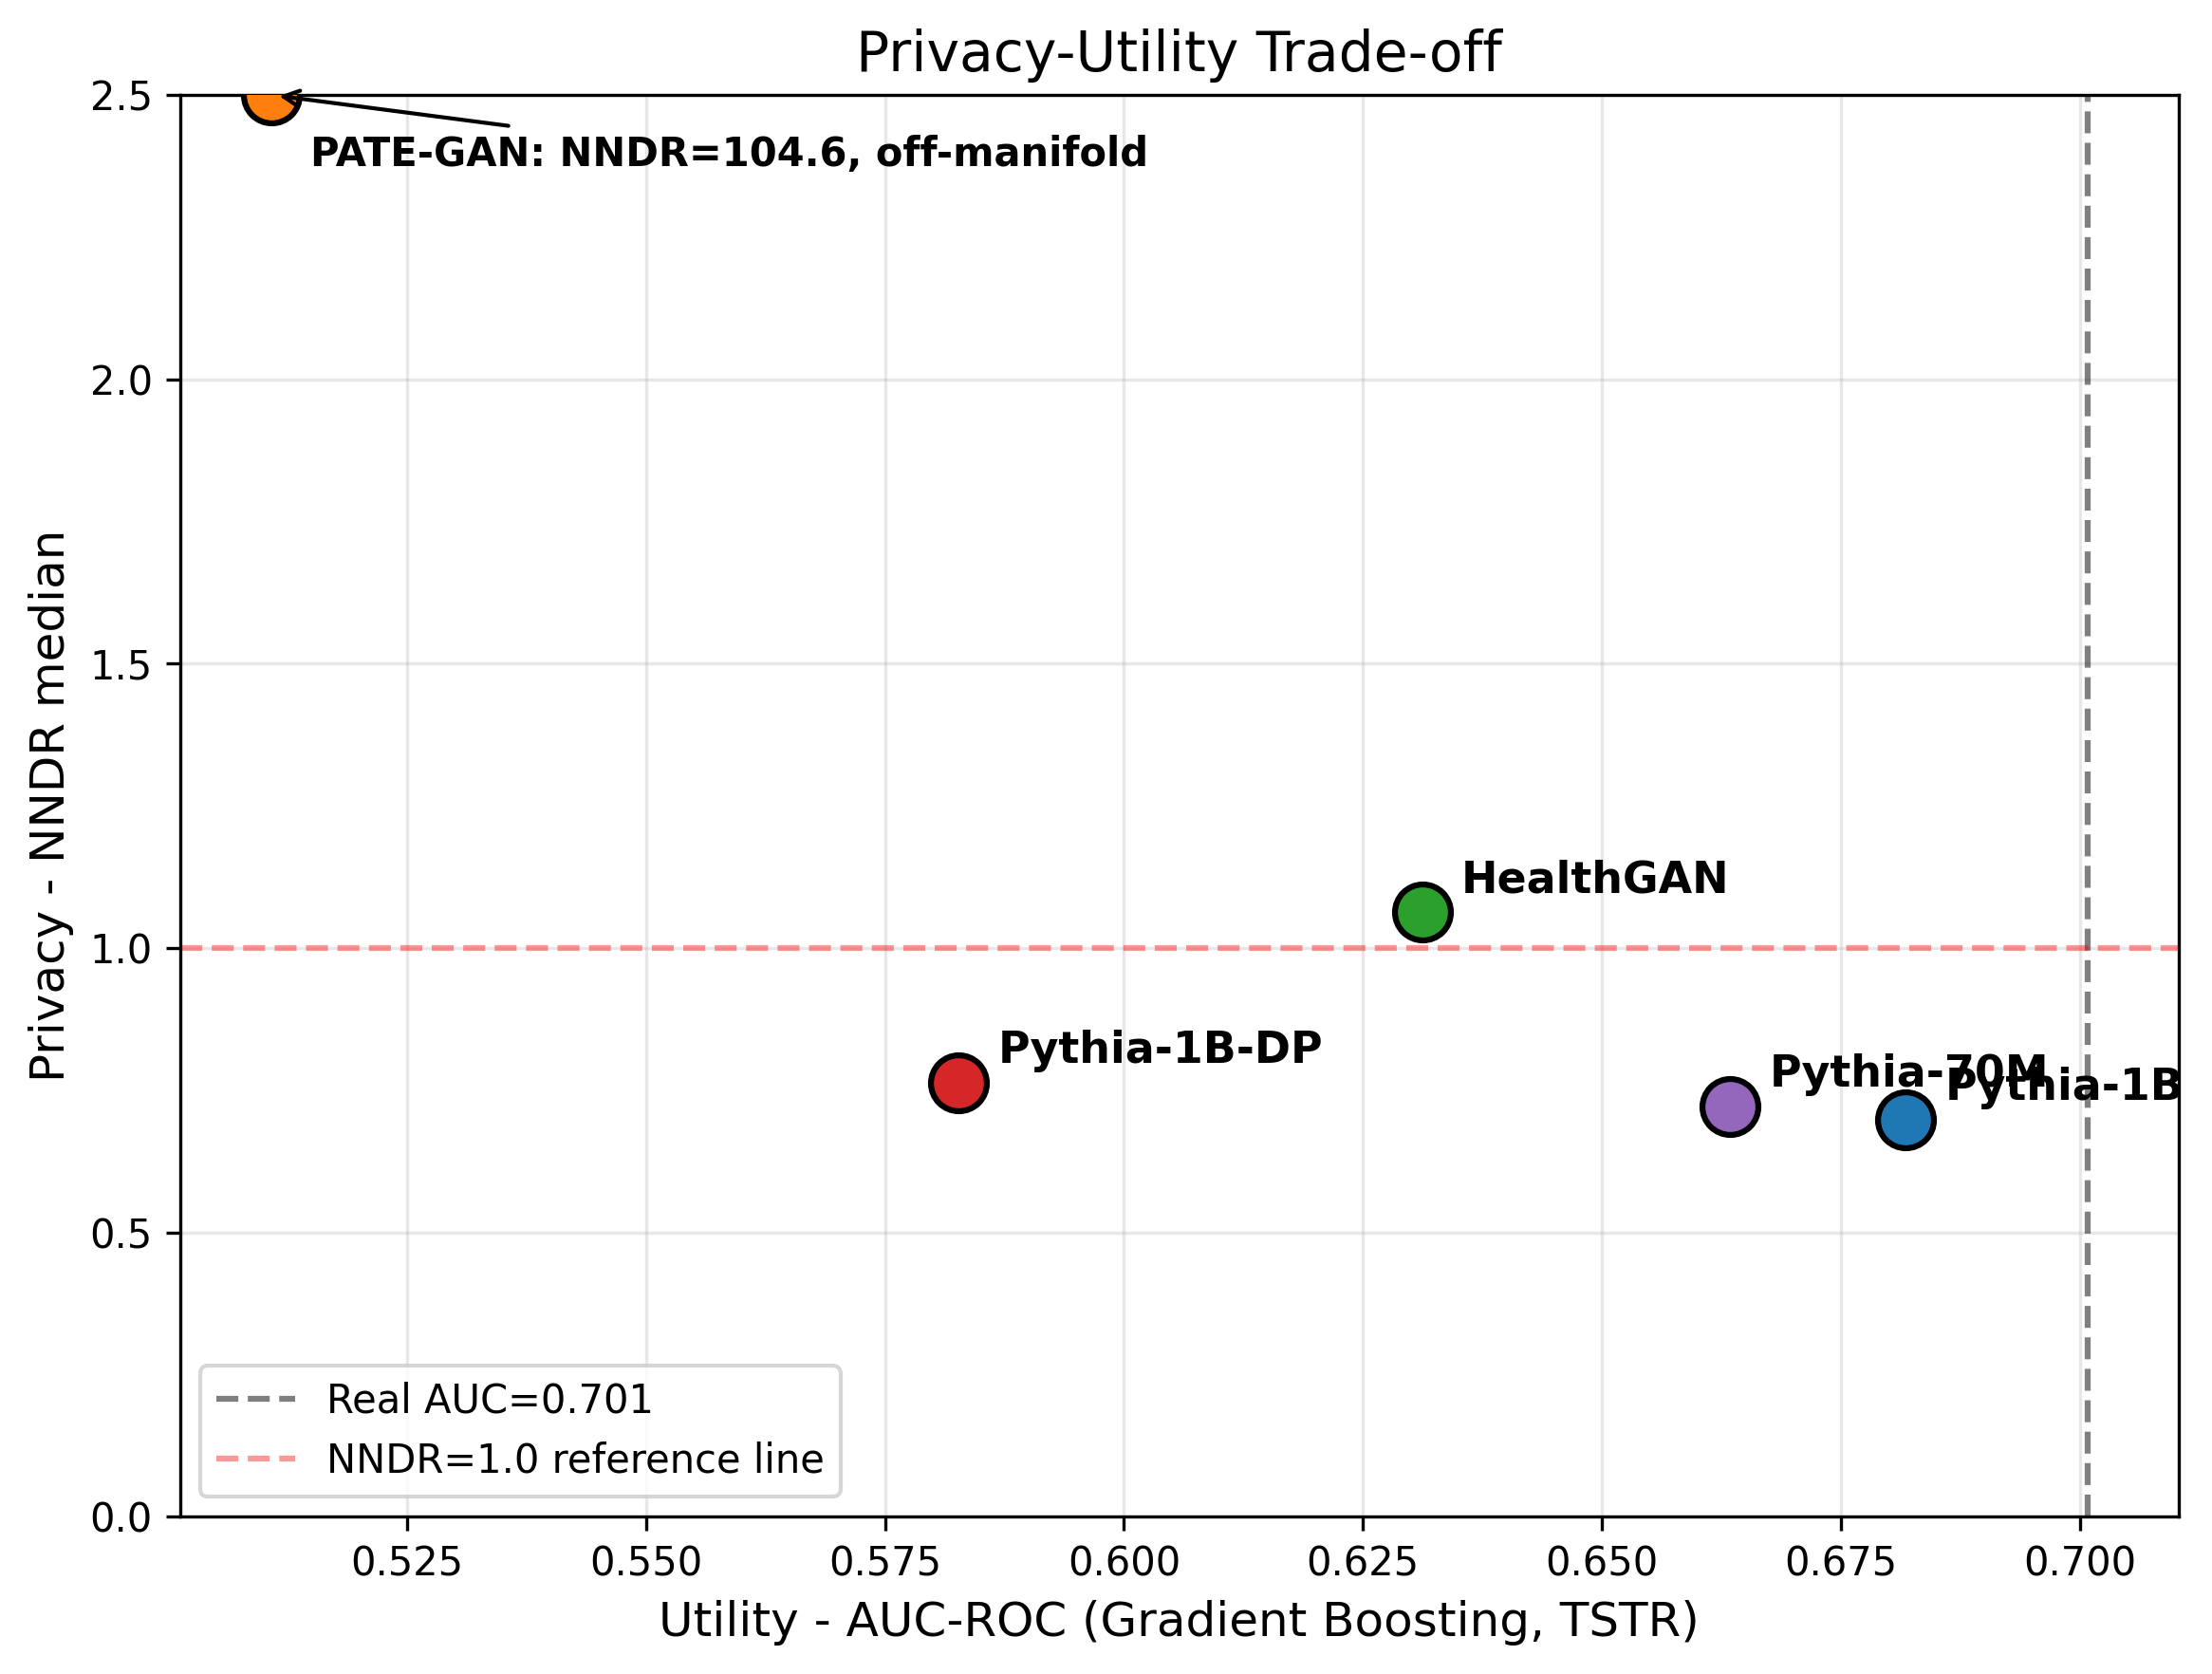
\includegraphics[width=0.85\textwidth]{images/results/4a-privacy_utility_landscape}
\caption{Privacy-utility landscape across the five generators. The
horizontal axis reports predictive utility (Gradient-Boosting TSTR
AUC-ROC), and the vertical axis reports median NNDR, where values above
$1.0$ indicate that the median synthetic-to-real distance is not below the
real-to-real reference scale. For readability, the PATE-GAN marker is shown
at a capped y-position. True median NNDR is $104.6$, as indicated by
the annotation. This inflated value reflects off-manifold output rather
than usable privacy protection. PATE-GAN is included for landscape
completeness and interpreted as the GAN family's DP-enforced operating
point (\S\ref{sec:discussion:limit:pategan-dual-role}).}
\label{fig:rq2:landscape}
\end{figure}

The plane separates into two regimes. PATE-GAN occupies an isolated
position high on the privacy axis (NNDR $\approx 105$) but at the lowest
utility (AUC $0.511$). As established in
Section~\ref{sec:results:rq2:privacy}, its extreme distance ratio is an
artefact of distributional collapse rather than genuine protection. The
remaining four generators lie close together near the NNDR unity reference
line and spread along the utility axis: Pythia-1B-DP at the low-utility end (AUC
$0.583$), then HealthGAN ($0.631$), Pythia-70M ($0.663$), and Pythia-1B
($0.682$) closest to the real-data ceiling. Among these usable
generators, HealthGAN alone sits at or above the NNDR unity reference line
(NNDR $1.063$), while the three Pythia variants fall just below it (NNDR
$0.70$-$0.76$). No single family dominates this selected two-axis plane.
LLM family supplies the highest-utility operating points, whereas
GAN family supplies the only usable point above the NNDR unity reference
line.

\paragraph{Utility Radar Comparison:}
\label{sec:results:rq2:radar}

Figure~\ref{fig:rq2:radar} overlays the five generators across six
normalised utility axes: AUC-ROC, F1, marginal fidelity ($1-$mean KS),
correlation preservation ($1-$CorrDiff), Cox confidence-interval overlap,
and feature-importance agreement. Each axis is min-max scaled to
$[0,1]$, with the real TRTR result used as a scaling anchor where
applicable but not plotted as a generator. Privacy metrics are excluded
from this radar because several privacy diagnostics have threshold-based
or two-sided interpretations and are therefore less suitable for a single
``larger is better'' radial display.

\begin{figure}[H]
\centering
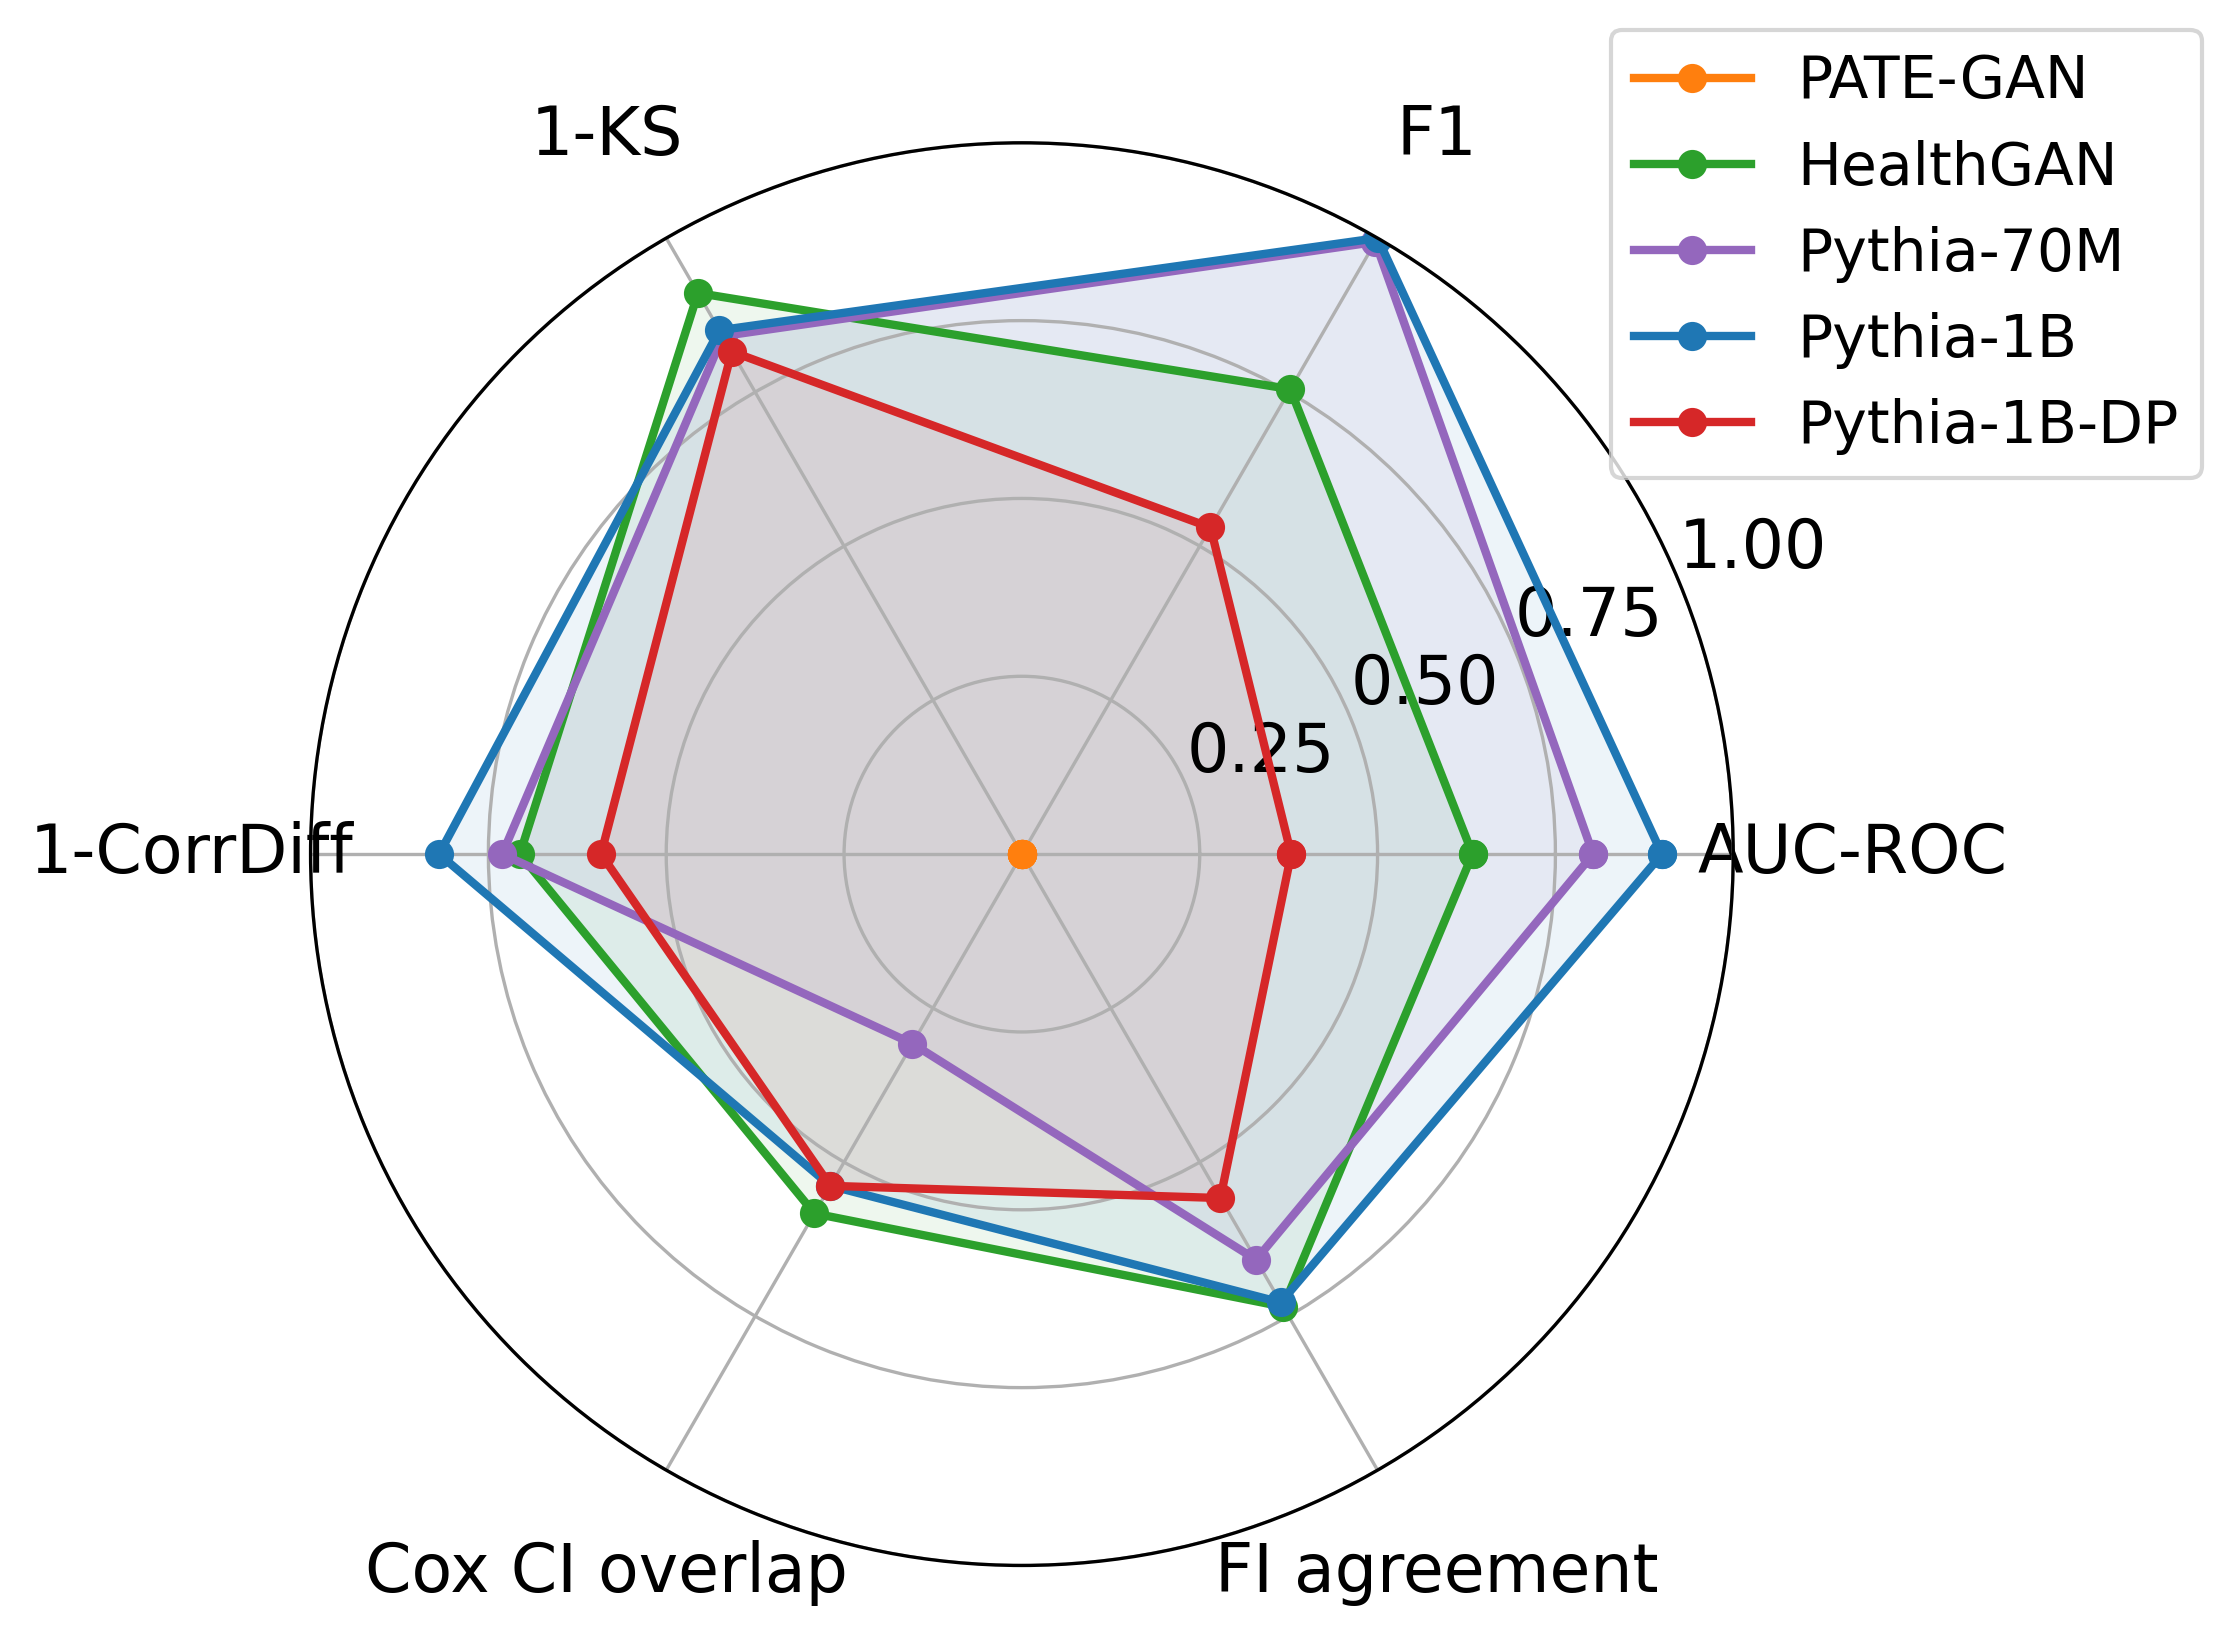
\includegraphics[width=0.78\textwidth]{images/results/4b-utility_radar}
\caption{Utility Radar Comparison across six min-max scaled utility axes:
AUC-ROC, F1, $1-$KS, $1-$CorrDiff, Cox confidence-interval overlap, and
feature-importance agreement. Larger radius indicates stronger relative
utility on the plotted axis.}
\label{fig:rq2:radar}
\end{figure}

The radar should be interpreted as a qualitative profile view rather than a scalar ranking.
The main advantage is, differently scaled utility measures can be
inspected on a common visual scale. It makes broad and narrow utility
profiles easier to compare. The limitation of this evaluation is that min-max scaling is
relative to the models included in the figure and does not preserve the
absolute distances of the original metrics. The polygon area should
therefore not be read as a formal performance score.

The pattern is consistent with the preceding utility results. PATE-GAN
sits at the centre because it is the lowest of the five generators on every
utility axis, which min-max scaling maps to zero. This is a relative floor
rather than zero utility, and the underlying values (for example TSTR
AUC-ROC $0.511$) are reported in Table~\ref{tab:rq2:summary}. Its central
position reflects weak predictive transfer, poor correlation preservation,
and the absence of Cox confidence-interval overlap. The non-collapsed generators form broader
profiles. Pythia-1B has the strongest relative profile on AUC-ROC, F1,
and correlation preservation, with high feature-importance agreement.
HealthGAN has the strongest relative marginal fidelity and Cox
confidence-interval overlap. Pythia-1B-DP remains non-collapsed but is
lower than Pythia-1B on the two predictive axes, which is consistent with
the TSTR utility cost reported above.

\paragraph{Utility-Privacy Heatmap:}
\label{sec:results:rq2:heatmap}

Figure~\ref{fig:rq2:heatmap} provides the metric-level inspection view
defined in Section~\ref{sec:eval:aggregate:heatmap}. Each metric is
min-max scaled to $[0,1]$ across the generators. The orientation
of the two blocks are different. Utility metrics are shown as performance, so a larger
value is better. Privacy metrics are shown as risk, so a larger
value is worse. Here only the leakage side of the middle-ideal privacy
metrics counted. The display
therefore exposes the full per-metric pattern without collapsing the
metrics into a single composite score.

\begin{figure}[H]
\centering
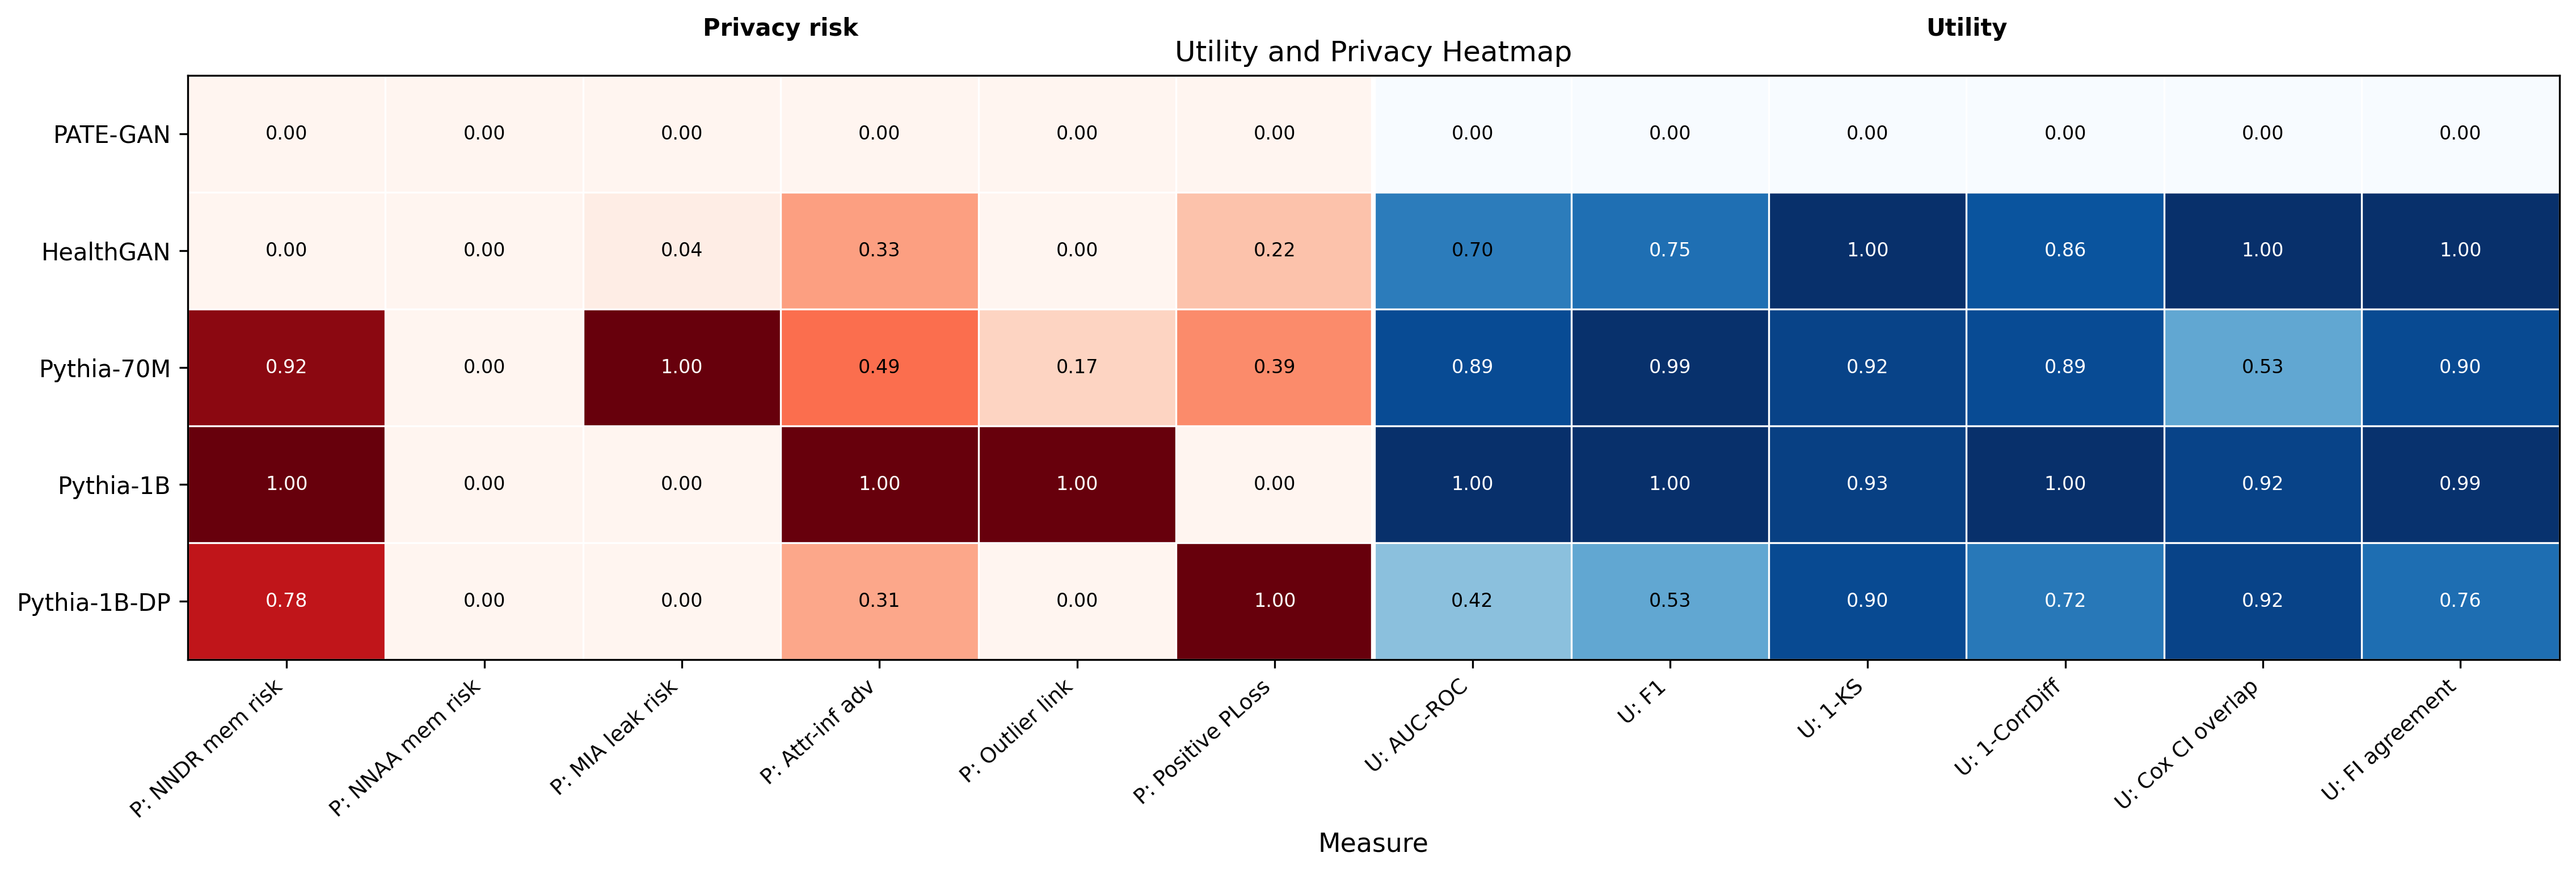
\includegraphics[width=0.90\textwidth]{images/results/4e-utility_privacy_heatmap}
\caption{Utility-privacy heatmap across the five generators. Utility
metrics are oriented as performance and privacy metrics as risk, each
min-max scaled to $[0,1]$ across the generators. Darker cells indicate 
better utility but greater privacy risk. Therefore,
dark utility and pale privacy cells are preferred. Only the leakage side of
the middle-ideal privacy metrics is counted, so a distributionally
collapsed generator can appear low-risk in the privacy block and must be
read together with the summary table of Table~\ref{tab:rq2:summary}.}
\label{fig:rq2:heatmap}
\end{figure}

The heatmap confirms the patterns observed in the individual metrics.
However, because each column is min-max scaled across the generators, the
colours represent relative rather than absolute differences. On the utility
side, PATE-GAN performs substantially worse than the other four generators
across both similarity and predictive metrics.

Most privacy values are close to their reference levels
(Table~\ref{tab:rq2:summary}). So, the colour scale can make small
privacy differences appear larger than they are. The Pythia variants show
the strongest relative proximity signal because their NNDR values are
below $1.0$. Pythia-70M has the highest relative membership-inference
signal, while Pythia-1B has the highest attribute-inference and outlier-
linkability signals. These signals are reduced or absent in Pythia-1B-DP.

PATE-GAN appears pale in the privacy block because its records are far from
the real-data distribution, not because it provides stronger practical
privacy. A pale cell therefore indicates low utility in the utility block
but low apparent risk in the privacy block. The heatmap should
be interpreted as a relative comparison and read together with the raw
values in Table~\ref{tab:rq2:summary}.

\paragraph{Pareto Analysis:}
\label{sec:results:rq2:pareto}

To examine the privacy and utility balance in RQ2, Pareto analysis is
applied to the two axes shown in Figure~\ref{fig:rq2:landscape}.
Gradient-Boosting TSTR AUC-ROC represents utility, while median NNDR
represents privacy. The analysis follows the rule defined in
Section~\ref{sec:eval:aggregate:tradeoff}. A generator is Pareto-optimal
when no other generator performs at least as well on both axes and better
on one.

Using all five generators, the Pareto frontier includes PATE-GAN,
HealthGAN, Pythia-70M, and Pythia-1B. Pythia-1B-DP is the only dominated
generator because HealthGAN achieves higher utility ($0.631$ versus
$0.583$) and a higher NNDR ($1.063$ versus $0.763$). PATE-GAN appears on
the frontier only because its output produces an extremely high NNDR. Its
output differs greatly from the real-data distribution, so it is not
considered a usable solution. After excluding PATE-GAN, the usable
frontier contains HealthGAN, Pythia-70M, and Pythia-1B. The two
non-private LLMs provide higher utility, while HealthGAN provides the
higher NNDR.

The dominance of Pythia-1B-DP applies only to this AUC-ROC and NNDR
comparison. NNDR does not capture all forms of privacy protection,
including the reduction in attribute-inference leakage achieved by
Pythia-1B-DP
(Section~\ref{sec:results:rq2:privacy:aia}). Therefore, this result does
not show that differential privacy is generally ineffective. Its broader
costs and benefits are examined in Section~\ref{sec:results:rq3}.

\subsection*{Findings for Research Question 2}
\label{sec:results:rq2:answer}

RQ2 does not identify one universally superior generator family. Instead,
the evaluated configurations occupied different positions in the
privacy-utility trade-off. The non-private Pythia models provided the
strongest downstream predictive utility and pairwise linear-dependency
preservation, whereas HealthGAN provided the strongest marginal fidelity
and the better record-proximity profile among the usable
generators. The comparison therefore identifies different options
depending on whether the intended use prioritises statistical resemblance,
predictive performance, or empirical privacy risk.

Pythia-1B achieved the highest Gradient-Boosting TSTR
AUC-ROC ($0.6818$) and the lowest pairwise correlation difference
($0.0206$) when we are comparing on the utility side.
Pythia-70M followed with an AUC-ROC of $0.6634$ and similarly
strong downstream performance. HealthGAN achieved a lower AUC-ROC
($0.6312$) but produced the best marginal-distribution fidelity with a
mean KS statistic of $0.0480$. It also achieved the highest
feature-importance agreement ($0.914$). Although Pythia-1B was practically
similar at $0.911$. HealthGAN additionally had highest Cox
confidence-interval overlap. However, because the fitted duration was
time in hospital rather than time to readmission, this result is treated
only as a model-specific association diagnostic and not as clinical
survival evidence.

The selected privacy metrics separated the usable generators less clearly.
Membership-inference AUC remained close to $0.5$, and NNAA privacy loss
remained close to zero across all configurations. HealthGAN's median NNDR
of $1.063$ was closest to the real-data spacing reference of one. It also
showed no positive attribute-inference advantage and zero outlier
linkability. Pythia-1B had a lower NNDR of $0.698$, which indicates greater proximity
between synthetic and real records. It also had the highest observed
attribute-inference advantage of $0.0410$, mainly for the diagnosis
attribute. It had the highest outlier linkability, although the
absolute value remained low at $0.6\%$. These results do not establish
that HealthGAN is secure or that Pythia-1B is unsafe. They indicate that
Pythia-1B produced the clearest relative privacy-risk signals under the
specified attacks and linkability definition.

Pythia-70M occupied an intermediate trade-off position. Its predictive
utility was close to that of Pythia-1B, while its attribute-inference
advantage ($0.0064$) and outlier linkability ($0.1\%$) were lower.
The model therefore remained non-dominated in the primary AUC-ROC-NNDR Pareto
analysis, although it did not lead either predictive utility or
real-reference proximity. PATE-GAN was not considered a meaningful
privacy-utility option because its apparently favourable distances and
zero outlier linkability resulted from distributional collapse rather
than usable privacy protection.

Pythia-1B-DP represents a separate decision case. Compared with Pythia-1B,
the model reduced the maximum attribute-inference advantage from $+0.0410$ to
$-0.0056$ and outlier linkability from $0.6\%$ to zero. On the contrary, its
predictive utility decreased from $0.6818$ to $0.5827$. It is therefore relevant
when a formal differential-privacy requirement takes precedence, but it
does not provide the strongest observed predictive utility. The detailed
within-family consequences of differential privacy are addressed in
Section~\ref{sec:results:rq3}.

Overall, HealthGAN provides a more conservative balance between privacy
and utility. Pythia-1B is the preferred
option when predictive utility is the main priority and its higher
observed attribute-inference and outlier-linkability signals are
considered acceptable for the intended use and governance setting.
These recommendations are limited to the evaluated configurations,
dataset, metrics, and attacks. Because the results are based on single
point estimates without repeated-run uncertainty. Also, small numerical
differences should not be interpreted as statistically established
family-level effects.


\section{RQ3 - The Cost of DP Enforcement, Within-Family}
\label{sec:results:rq3}

% RQ3 (finalised): "At a matched privacy budget (ε=5.0), how does enforcing
% differential privacy using mechanisms appropriate to each family affect
% utility, and how do the resulting privacy-utility profiles differ
% between GAN-based (PATE-GAN vs HealthGAN) and LLM-based (Pythia 1B-DP vs
% Pythia 1B) synthesisers of tabular medical data?"
%
% The four generators analysed in this section are a subset of the five
% reported in \S\ref{sec:results:rq2}; the same experimental outputs are
% re-examined under a within-family DP-toggle lens, not re-run. Pythia-70M
% is excluded from RQ3's main comparison because DP-SGD failed at that
% scale (\S\ref{sec:results:rq3:pythia-70m-failure}).

\subsection{Convergence Failure of DP-SGD at the Pythia-70M Scale}
\label{sec:results:rq3:pythia-70m-failure}

An initial attempt to apply DP-SGD to Pythia-70M at $\varepsilon = 5.0$
failed to train usefully. The recorded training loss worsened across the
five epochs (from $3.38$ to $3.74$, peaking at $3.79$) under the
calibrated noise multiplier $\sigma = 0.436$, and the model did not
converge to a useful synthesis distribution. This suggests that the 
added noise may have weakened the useful gradient
signal at this model scale. However, gradient magnitudes were not measured
directly. The LLM-side DP comparison was therefore scaled to
Pythia-1B, which trained successfully under DP-SGD at the same privacy
budget. The finding from this is DP-SGD on small LLMs couldn't be 
applied at $\varepsilon = 5.0$. It is consistent with prior work
showing that larger LLMs tolerate DP noise more
gracefully~\cite{Li2022LargeDP}. The methodological consequence, that the
LLM-family DP toggle is operationalised at the 1B scale, is discussed in
\S\ref{sec:methods:pythia-dp:why-1b}.

\subsection{Cost of Differential Privacy on the GAN Family}
\label{sec:results:rq3:gan-toggle}

The GAN comparison examines the non-private HealthGAN and the
differentially private PATE-GAN. It shows the changes associated with
moving to a formally private GAN. However, because the models use
different architectures, these changes cannot be attributed to
differential privacy alone.
Table~\ref{tab:rq3:gan-toggle} reports the change on each headline metric.

\begin{table}[H]
\centering
\small
\caption{Within-family differential-privacy transition for the GAN family
(HealthGAN to PATE-GAN). $\Delta$ is PATE-GAN value minus 
HealthGAN value. On a utility row a negative $\Delta$ denotes a loss. 
The NNDR change should not be interpreted as a privacy improvement because
PATE-GAN's extremely high value results from its distance from the
real-data distribution. }
\label{tab:rq3:gan-toggle}
\begin{tabular}{lccc}
\toprule
Metric & HealthGAN & PATE-GAN & $\Delta$ \\
\midrule
Mean KS $\downarrow$       & 0.0480 & 0.5381 & $+0.4901$ \\
Corr.\ diff.\ $\downarrow$ & 0.0336 & 0.1142 & $+0.0806$ \\
AUC-ROC $\uparrow$         & 0.6312 & 0.5108 & $-0.1204$ \\
F1 $\uparrow$              & 0.3824 & 0.0093 & $-0.3731$ \\
Cox CI overlap $\uparrow$  & 0.5833 & 0.0000 & $-0.5833$ \\
NNDR median                & 1.063  & 104.601 & $103.538$ \\
Max.\ attr.\ adv.\ $\downarrow$ & $-0.0040$ & $-0.0266$ & $-0.0226$ \\
\bottomrule
\end{tabular}
\end{table}

Utility declines across all measures in this transition. Mean KS increases
from $0.0480$ to $0.5381$, while the correlation difference increases from
$0.0336$ to $0.1142$. AUC-ROC falls by $0.1204$ to near chance, F1
decreases from $0.3824$ to $0.0093$, and Cox confidence-interval overlap
falls from $7/12$ to $0/13$.

NNDR increases from $1.063$ to $104.601$. However, this does not represent
a genuine privacy improvement because PATE-GAN's output lies far from the
real-data distribution. The other privacy measures
change only slightly because both generators show low membership and
attribute-inference risks.

This is not a controlled comparison of differential privacy because
HealthGAN and PATE-GAN use different architectures. Therefore, the
observed utility loss cannot be attributed to differential privacy alone
(Section~\ref{sec:discussion:limit:gan-toggle-asymmetry}).

\subsection{Cost of Differential Privacy on the LLM Family}
\label{sec:results:rq3:llm-toggle}

The LLM-family comparison contrasts the non-private Pythia-1B with the
differentially private Pythia-1B-DP. Because both variants share the same
Pythia-1B backbone, the same row-as-text serialisation, and the same
low-rank fine-tuning configuration. This comparison is a
differential-privacy toggle. The only material difference is the DP-SGD
training procedure and some fine tuning parameters to accommodate DP-SGD. The private
variant was trained under a privacy budget that the accounting reports as
an achieved $\varepsilon = 4.998$ against a target of $5.0$ (with
$\delta = 10^{-5}$, gradient-clipping norm $1.0$, noise multiplier
$0.789$, and an effective batch size of $512$).
Table~\ref{tab:rq3:llm-toggle} reports the change on each headline metric.

\begin{table}[H]
\centering
\small
\caption{Within-family differential-privacy transition for the LLM family
(Pythia-1B to Pythia-1B-DP), a toggle on a shared backbone at
achieved $\varepsilon = 4.998$. $\Delta$ is the private value minus the
non-private value.}
\label{tab:rq3:llm-toggle}
\begin{tabular}{lccc}
\toprule
Metric & Pythia-1B & Pythia-1B-DP & $\Delta$ \\
\midrule
Mean KS $\downarrow$       & 0.0805 & 0.0992 & $+0.0187$ \\
Corr.\ diff.\ $\downarrow$ & 0.0206 & 0.0466 & $+0.0260$ \\
AUC-ROC $\uparrow$         & 0.6818 & 0.5827 & $-0.0991$ \\
F1 $\uparrow$              & 0.5036 & 0.2714 & $-0.2322$ \\
Cox CI overlap $\uparrow$  & 0.5385 & 0.5385 & $\phantom{+}0.0000$ \\
NNDR median                & 0.698  & 0.763  & $+0.065$ \\
Max.\ attr.\ adv.\ $\downarrow$ & $+0.0410$ & $-0.0056$ & $-0.0466$ \\
Outlier link.\ \% $\downarrow$  & 0.6 & 0.0 & $-0.6$ \\
\bottomrule
\end{tabular}
\end{table}

The cost is real and falls almost entirely on the predictive branch, where
it is uneven. AUC-ROC drops by a moderate $0.0991$ (to $0.5827$, still well
above chance), whereas F1 falls more steeply from $0.5036$ to $0.2714$,
close to a halving. The statistical-similarity branch
is barely affected (mean KS rises by only $0.0187$ and the correlation
difference by $0.0260$, both leaving the private variant comfortably within
the regime), and the survival model is untouched, with identical
confidence-interval overlap ($7/13$) before and after. On the privacy side
the toggle produces a small genuine benefit. The attribute-inference signal 
observed for primary diagnosis in the
non-private model was no longer detected under private training. The
maximum observed advantage decreased from $+0.0410$ to $-0.0056$, while
outlier linkability decreased to zero. Differential
Private training reduced predictive utility within the LLM family. The
reduction was moderate for AUC-ROC but larger for F1. However, it also
reduced the observed attribute-disclosure risk while broadly preserving
distributional fidelity and Cox-model agreement.

\subsection{Cross-Family Comparison of Differential-Privacy Cost}
\label{sec:results:rq3:arrow-plot}

Figure~\ref{fig:rq3:arrow} places the four generators on the
privacy-utility plane of Figure~\ref{fig:rq2:landscape} and draws each
within-family differential-privacy transition as an arrow from the
non-private to the private variant. The vertical axis (NNDR) is shown on a
logarithmic scale so that both transitions are visible despite PATE-GAN's
off-scale distance ratio.

\begin{figure}[!htbp]
\centering
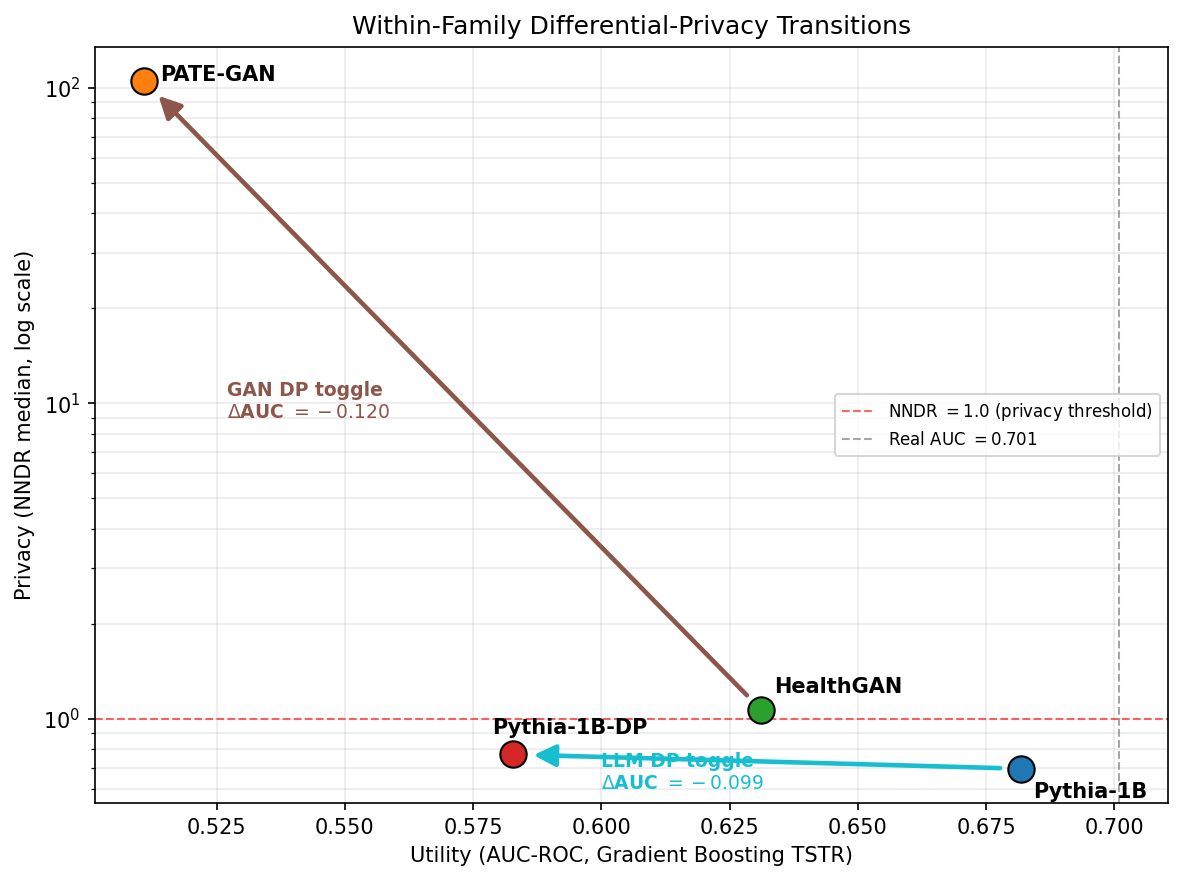
\includegraphics[width=0.82\textwidth]{images/results/arrow}
\caption{Within-family differential-privacy changes on the privacy and
utility plane. The arrows compare HealthGAN with PATE-GAN for the GAN
family and Pythia-1B with Pythia-1B-DP for the LLM family. The vertical
axis uses a logarithmic scale. PATE-GAN's high NNDR reflects its large
distance from the real-data distribution, as discussed in
Section~\ref{sec:results:rq2:privacy}.}
\label{fig:rq3:arrow}
\end{figure}

The two arrows differ sharply in length and meaning. The LLM arrow is
short and almost horizontal. It moves left by $0.0991$ in utility and only
slightly upward in NNDR, a controlled step that keeps the private variant
within the usable region of the plane. The GAN arrow is long and steep,
moving the operating point from HealthGAN's usable position down and to the
left to PATE-GAN's degenerate position. As noted, its vertical extent
reflects the off-manifold distance artefact rather than a genuine privacy
gain. Read together, the figure shows
that the controlled, architecture-matched differential-privacy step (the
LLM arrow) is far less destructive to utility than the GAN-side
transition, and that the only differentially private generator to remain
in the usable region of the plane is the LLM one.

\subsection{Supplementary Per-Family Analyses}
\label{sec:results:rq3:supplementary}

The full per-generator diagnostics underlying both transitions are
referenced rather than re-plotted here. The complete metric values for all
four generators appear in the comprehensive summary of
Table~\ref{tab:rq2:summary}. The per-generator correlation-difference
heatmaps and Cox hazard-ratio plots for HealthGAN, PATE-GAN, Pythia-1B, and
Pythia-1B-DP are collected in Appendix~\ref{app:utility-diag}, where the
two within-family pairs can be compared panel by panel.

\subsection*{Findings for Research Question 3}
\label{sec:results:rq3:answer}

At the same target privacy budget of
$(\varepsilon,\delta)=(5.0,10^{-5})$, the two model families showed
notably different privacy-utility trade-offs. 
The Pythia-1B transition kept statistical fidelity
comparatively well and improved selected empirical privacy diagnostics,
but incurred a substantial reduction in predictive utility. In contrast,
the HealthGAN-to-PATE-GAN transition was associated with a much broader
loss of fidelity and utility. However, because the GAN configurations
also differ in architecture and training procedure, this deterioration
cannot be attributed to differential privacy alone.

Within the LLM family, Pythia-1B-DP had a TSTR AUC-ROC decrease of
$0.0991$ and an F1 decrease of $0.2322$ relative to Pythia-1B. Mean KS
increased by $0.0187$ and pairwise correlation difference increased by
$0.0260$. It indicates smaller losses in marginal and linear-dependency
fidelity than in predictive performance. Cox confidence-interval overlap
remained unchanged at $7/13$.

The LLM-side privacy improvement was selective rather than consistent
across all metrics. For Pythia-1B-DP, the maximum attribute-inference advantage decreased
from $+0.0410$ to $-0.0056$. This result indicates that the evaluated
attack did not outperform the baseline. Outlier linkability also
decreased from $0.6\%$ to zero. Median NNDR moved from $0.698$ to
$0.763$ which is towards the real-to-real spacing reference. In contrast,
membership-inference AUC remained effectively unchanged at approximately
$0.5$, and NNAA privacy loss remained close to zero for both variants.
NNAA test accuracy increased from $0.6204$ to $0.7139$, showing that the
private synthetic data became easier to distinguish from real data.
Differential privacy therefore improved the observed attribute- and
outlier-specific risks, but did not improve every empirical privacy
dimension.

Within the GAN family, HealthGAN to PATE-GAN transition was
associated with substantially larger utility and fidelity losses.
AUC-ROC decreased by $0.1204$, F1 decreased by $0.3731$, mean KS
increased by $0.4901$, and pairwise correlation difference increased by
$0.0806$. Cox confidence-interval overlap also changed from $7/12$ to
$0/13$. PATE-GAN's median NNDR increased from $1.063$ to $104.601$, but
this cannot be interpreted as an empirical privacy improvement. The
extreme distance occurred together with an NNAA test accuracy of $0.9999$
indicates that PATE-GAN generated records
far outside the real-data distribution. Its zero outlier linkability is
therefore uninformative.

Comparing the resulting private configurations, Pythia-1B-DP retained
substantially higher predictive and statistical-similarity utility than
PATE-GAN. It achieved an AUC-ROC of $0.5827$ compared with $0.5108$, an
F1 score of $0.2714$ compared with $0.0093$, a mean KS of $0.0992$
compared with $0.5381$, and a correlation difference of $0.0466$
compared with $0.1142$. Thus Pythia-1B-DP remained within a usable, utility-reduced region
of the privacy-utility profile, whereas PATE-GAN did not at the same privacy budget.

These findings provide stronger evidence about the DP-SGD-associated
change within the LLM family because the Pythia variants share the same
backbone and data representation. The GAN comparison instead combines 
the effects of architecture, training
procedure, and privacy mechanism. Consequently,
the results do not constitute a controlled comparison of DP-SGD and PATE,
nor do they show that one mechanism is generally superior. They show that,
for the evaluated configurations, the LLM-based private model degraded
more gracefully under the matched target privacy budget. The failed
Pythia-70M DP-SGD run further indicates that this result should not be
generalised across LLM scales. All reported differences remain
descriptive point estimates without repeated-run uncertainty and are
limited to the evaluated utility and privacy metrics.

\cleardoublepage

    % !TEX root = ../thesis.tex

\chapter{Discussion}
\label{ch:discussion}

% Where the Results chapter reports numbers, this chapter interprets them,
% situates the findings against prior work, and acknowledges limits.

\section{Interpretation of Results per Research Question}
\label{sec:discussion:interpretation}

\subsection{RQ1: Complementary Evaluation Metrics}

The clearest methodological finding from RQ1 is that a
distance-based privacy result cannot be interpreted as evidence of
protection when the synthetic data have poor fidelity. PATE-GAN is
a direct example for this case. It produced large nearest-neighbour distances and zero
outlier linkability. From this evidence alone one can conclude that PATE-GAN
is the obvious choice, but when you include fidelity analysis it shows substantial distributional
differences and weak predictive utility. Its distance results therefore
reflected poor similarity to the real data rather than a
favourable privacy and utility balance.

The other privacy diagnostics also had different roles. Membership
inference and NNAA privacy loss provided little separation between the
generators under the selected attacks. NNDR and attribute inference
identified some model-specific differences. These findings show why
privacy metrics should be interpreted together and alongside utility
results. This supports previous recommendations for multidimensional
synthetic-data evaluation
\cite{hernandez2022synthetic,lautrup2025syntheval}.

The conclusions also depend on how the metrics were implemented. Mean KS
was applied to nominal variables represented by numerical codes.
Correlation difference measured only pairwise Pearson relationships
between encoded columns. The privacy results depend on the selected
attacks, attributes, distance measure, and outlier definition. Future
work should use type-specific marginal distances, mixed-data association
measures, repeated runs, and stronger privacy attacks. These extensions
would show whether the current findings remain stable under different
evaluation choices.

\subsection{RQ2: Comparison of the Evaluated GAN and LLM Configurations}

The main finding from RQ2 is that utility separated the evaluated
configurations more clearly than the selected privacy attacks. The two
non-private Pythia configurations produced the highest observed
predictive-performance results. Pythia-1B also produced the lowest
pairwise linear-correlation difference. HealthGAN produced the lowest
observed mean KS and the highest Cox confidence-interval overlap.
Membership inference and outlier linkability provided less separation,
but NNDR and attribute inference identified some model-specific
differences.

These results do not identify a universal winner. Instead, they show
that the evaluated configurations preserved different properties of the
real data. The Pythia models performed more strongly on predictive
transfer and pairwise linear relationships. HealthGAN performed more
strongly on marginal similarity and Cox confidence-interval overlap.

A possible explanation for the Pythia results is that autoregressive,
class-conditioned generation retained conditional relationships that
were useful for downstream prediction. Because when generating each feature,
model uses both the class label and previously generated features.

HealthGAN's strong marginal  similarity may result from its GAN training
process, which encourages synthetic records to resemble the real data. In GAN training, 
differences in individual feature
distributions can help the discriminator identify synthetic records,
thereby encouraging the generator to reproduce the marginal
distributions of the real data. These explanations are plausible 
but were not tested directly. The
models also differed in architecture, scale, pretraining, representation,
optimisation, and computational cost. The observed differences therefore
cannot be attributed to the generator family alone.

The difference between F1 and AUC-ROC may result from the selected
classification threshold rather than better overall separation of the
two classes. In addition, each configuration was evaluated using a single recorded
run. The stability of the observed model ordering across random seeds was
therefore not tested.

Future studies should repeat the comparison across several clinical
datasets and random seeds. Training data, tuning effort, and
computational budgets should be controlled as well.
Scale-controlled LLM experiments would also help determine whether the
predictive pattern is associated with model size, as suggested by
previous work~\cite{Miletic2024}.

\subsection{RQ3: Observed Changes Under the Private Configurations}

The most informative RQ3 finding comes from the more closely matched
Pythia-1B comparison. The private configuration had lower predictive
performance than the non-private configuration. However, Cox
confidence-interval overlap remained unchanged, and the changes in
statistical similarity were smaller than the changes in predictive
performance. The unchanged Cox overlap is clinically relevant because it
shows that the same level of effect-interval agreement was observed in
both Pythia-1B configurations, even though their predictive results
differed. The reason for that could be that predictive performance 
requires multivariable relationships to be preserved. Statisical 
similarity don't necessarily gurantees that. Also for Cox
confidence-interval doesn't capture difference in interval width or 
the extent of overlap. 

For Pythia-1B-DP, the attribute-inference attack performed no better than
the baseline, and outlier linkability decreased to zero. These results
suggest lower disclosure risk under the selected metrics. However, other
privacy risks and the stability of these results across repeated runs were
not evaluated.

One possible explanation is that private fine-tuning was limited to the
low-rank adapter parameters of the pretrained Pythia-1B model. This may
have allowed the model to retain useful pretrained information while the
adapter updates were clipped and noised. The result is consistent with
previous evidence that larger pretrained language models can perform
better under private fine-tuning~\cite{Li2022LargeDP}. However, the
Pythia-70M and Pythia-1B private runs differed in dataset size, batch
construction, learning rate, and calibrated noise multiplier. Their
different training behaviour cannot therefore be attributed to model
scale alone.

Pythia-1B-DP also retained substantially more measured utility than
PATE-GAN. This cross-family comparison provides weaker evidence because
HealthGAN and PATE-GAN differ in architecture, training objective, and
privacy procedure. PATE-GAN's poor results may reflect its particular
implementation, the dataset, its optimisation settings, or a combination
of these factors. The result should not be interpreted as evidence that
PATE or differentially private GANs generally fail.

A further limitation concerns the scope of the Pythia privacy accounting.
The reported privacy cost applies to the DP-SGD parameter updates. The
loss-based checkpoint comparison was not included in that accounting.
The reported value should therefore not be presented as a complete
end-to-end privacy guarantee for every operation in the training
pipeline.

Future work should compare private and non-private versions of the same
GAN architecture. The analysis should also repeat the Pythia comparison using matched
batch-size and optimisation settings. It should evaluate multiple model
scales and privacy budgets and report uncertainty across repeated runs.
Stronger attacks and privacy-accounted model-selection procedures would
provide a more complete assessment of the relationship between formal
accounting and empirical disclosure risk.

\section{Strengths and Weaknesses of the Two Generator Families}
\label{sec:discussion:gan-vs-llm}

The results show that the two model families have different but
complementary strengths. The strength of the
GAN family is distributional where HealthGAN matches the real marginals more
tightly than any other generator and, once trained, samples cheaply. Its
weaknesses are equally visible here. It enforces no schema-level
constraints, and the only differentially private GAN evaluated does not
produce usable data at the tested budget. However, this result reflects both 
the differential-privacy mechanism
and the change in architecture. It therefore cannot be attributed to
differential privacy alone(\S\ref{sec:discussion:limit:gan-toggle-asymmetry}). 
The strength of the LLM family
is its native handling of mixed-type tabular data through a row-as-text
representation. The same model ingests categorical, ordinal, and continuous
fields without per-column encoders, learns their conditional structure, and
through schema-aware parsing, emits syntactically valid rows. This
representational flexibility underlies the predictive advantage of the LLM
family. Its graceful degradation under differential privacy has a distinct
cause. DP-SGD perturbs a small low-rank adapter at the $1$B
scale, rather than following from the text representation itself. Its
costs are a generation-time parsing-and-retry overhead. It also has substantially longer
training and inference, and a known problemn of word-for-word memorisation
of training text~\cite{Carlini2021Extracting}. Notably, however, the
membership-inference results reported here show no measurable memorisation by
any generator at this scale (\S\ref{sec:results:rq2:privacy:mia}).

\paragraph{Sensitivity to Categorical Granularity:}
The age-binning ablation
(Section~\ref{sec:results:rq2:utility:age-binning}) shows that upstream
categorical-cardinality choices can affect generators differently. Although
the comparison is limited to the two GAN baselines and Pythia-70M, the only
models for which matched three-bin and ten-bin runs exist. Restoring the
native ten-decade \emph{age} encoding raised the predictive utility
of Pythia-70M by $\approx 0.065$ and its F1 by $\approx 0.106$ which is the
largest AUC gain among the compared generators. HealthGAN responded on a
similar scale but in a mixed direction. It gains on F1 ($+0.118$) while
losing slightly on AUC ($-0.029$). PATE-GAN remained weak under
both encodings. No single family is therefore uniformly more sensitive on
this ablation. The practical implication for healthcare data stewards is
that preprocessing decisions
can shift recoverable downstream utility for some generators.

\section{Practical Recommendations for Healthcare Data Stewards}
\label{sec:discussion:recommendations}

The results translate into a small set of evidence-based recommendations
for a data steward choosing a generator for tabular medical data.

\paragraph{When a formal privacy guarantee is required:}
The differentially private LLM (Pythia-1B-DP) is the recommended choice
rather than the differentially private GAN as implemented here. At
$\varepsilon = 5.0$ the DP-LLM retained usable utility (TSTR AUC $0.583$)
and reduced attribute disclosure, whereas the PATE-GAN implementation
evaluated in this thesis collapsed to near chance on every utility metric.
These findings challenge the common use of DP-GAN as the default
approach. However, two caveats apply. First, the DP-LLM must have
sufficient model capacity, as DP-SGD training failed at the $70$M scale.
Second, the evidence for GANs is limited to the PATE-GAN configuration
evaluated in this study (\S\ref{sec:discussion:limit:gan-toggle-asymmetry}).

\paragraph{When maximum utility is required without a formal guarantee:}
Both models are reasonable choices, depending on the main objective.
Pythia-1B provides the highest predictive utility and the strongest
fidelity in joint feature relationships. In contrast, HealthGAN provides
the best marginal fidelity and is the only non-private configuration to
meet or exceed the NNDR reference value of one. It also requires only a
fraction of the computational cost of the LLM.
The choice is the genuine trade-off identified in RQ2 rather than a clear
winner.

\paragraph{When schema handling or operational simplicity dominates:}
The LLM generators ingest mixed-type data without per-column encoders and
emit schema-valid rows directly, which simplifies the pipeline at the cost
of generation time. The GAN requires an explicit encoding and decoding stage
but is far cheaper to run.

\paragraph{Outlier protection:}
No generator concentrated synthetic mass around the vulnerable tail of the
real distribution (outlier linkability $\leq 0.6\%$ for all), so outlier
disclosure was not a discriminating factor in this study. A steward with a
specific outlier-protection requirement should nonetheless verify it
directly, since this property is dataset-dependent.

\section{Toward Standardisation of Synthetic-Data Evaluation}
\label{sec:discussion:standardisation}

The evaluation framework assembled for this thesis, comprising two utility
branches (statistical similarity and predictive performance) and a privacy
pillar reported through twelve complementary single-number metrics. It is
offered as a step toward the reusable evaluation standard called for by
\textcite{hernandez2022synthetic}. General-purpose frameworks such as SynthEval
pursue this goal for arbitrary tabular data~\cite{lautrup2025syntheval}. 
This study applies the same two-part framework to a clinical benchmark
and uses it for a controlled comparison of GAN- and LLM-based approaches. 
Its central principle also applies here: no single metric is sufficient,
and the metrics must be considered together. The PATE-GAN results show
that evaluating fewer dimensions may favour generators that perform well
on one metric while producing data of poor overall quality. What would not
transfer unchanged is the domain-specific content of the suite. The
privacy thresholds (an NNDR of unity, the outlier radius) are calibrated to
the geometry of the real data and must be recomputed per dataset. 
The predictive-utility evaluation requires a predefined outcome
variable, which is used to train and assess the downstream prediction
models. In this study, the target variable is binary readmission. 
The framework should be understood as a reusable \emph{structure} that
jointly evaluates two utility dimensions and privacy. In this study, it
is implemented using metrics suitable for clinical tabular data with a
binary outcome.

\section{Limitations}
\label{sec:discussion:limitations}

\subsection{Single-Dataset Scope}
\label{sec:discussion:limit:dataset}

The entire study is conducted on a single dataset, the Diabetes 130-US
Hospitals dataset. It is a deliberate choice of a large
($> 70{,}000$-record), mixed-type clinical table with binarized
outcome. So it makes it a representative medical tabular testbed, but it is
not universal. The planned evaluation using MIMIC-III was reduced in scope.
Consequently, the findings, particularly the absolute utility values and
model-family rankings, may not generalise to datasets with substantially
different dimensionality, sparsity, or outcome structures.

\subsection{Upper Bound on Language-Model Scale}
\label{sec:discussion:limit:pythia-size}

The LLM-side evaluation is capped at the Pythia-1B scale. 
Pythia-1B was included as a larger non-private and private comparison
point than Pythia-70M. This increase in scale was motivated by the
failure of DP-SGD training at the $70$M scale, as reported in
\S\ref{sec:results:rq3:pythia-70m-failure}. However, larger decoder-only
models with several billion parameters, such as Llama- or Qwen-based
models, were not evaluated. The findings on
the LLM side should therefore be read as characterising the small-to-mid LLM
regime. Model size has been correlated with higher gains, so the
absolute utility figures here are likely a lower bound on what comparable
LLM-based synthesisers can attain at greater scale\cite{Miletic2024} .

\subsection{Architectural Asymmetry of the Cross-Family DP Comparison}
\label{sec:discussion:limit:gan-toggle-asymmetry}

The GAN-family DP comparison reported in
\S\ref{sec:results:rq3:gan-toggle} combines architectural and mechanism
differences. HealthGAN and PATE-GAN are not the same architecture with
differential privacy toggled on or off, but distinct generative designs.
The LLM-family comparison
(\S\ref{sec:results:rq3:llm-toggle}) is, on the contrary, an
architecture-controlled toggle. Pythia-1B and Pythia-1B-DP share the same
decoder-only backbone, the same Tabula serialisation, and the same LoRA
fine-tuning configuration. Although their Fine tuning configuration 
has some differences, but that is due to accommodating DP-SGD in the Pipeline.
So, the observed difference between them is
the DP-SGD training procedure. This asymmetry was difficult to avoid because PATE-GAN has no
standardised non-private counterpart, while applying DP-SGD to WGAN-GP
presents technical challenges, as discussed in
\S\ref{sec:methods:healthgan:nodp}. However, this limitation should be considered when comparing the utility
cost of differential privacy across the two model families. Part of the
GAN-side utility difference reported in
\S\ref{sec:results:rq3:gan-toggle} may result from the architecture change
rather than from differential privacy alone. A further caveat concerns the PATE-GAN
implementation itself. The original PATE-GAN study reported useful 
synthetic-data utility under
stricter privacy budgets than the budget used here~\cite{pategan}.
However, the configuration evaluated in this thesis collapsed on the
current benchmark. This configuration used linear logistic-regression
teachers that were refitted at each training round and a weight-clipped
Wasserstein student
(\S\ref{sec:methods:pategan:teacher}). The observed collapse should therefore be read
as a property of this implementation, dataset, and budget, not as evidence
that differentially private GANs fail in general.

\subsection{Dual Role of PATE-GAN in the Landscape Comparison}
\label{sec:discussion:limit:pategan-dual-role}

PATE-GAN appears alongside non-private models in the RQ2 landscape view
(\S\ref{sec:results:rq2:landscape}) even though it incorporates differential
privacy by construction. This is a reporting choice rather than a flaw.
PATE-GAN is the de-facto DP-GAN baseline in the literature~\cite{pategan},
and excluding it from the landscape figure would make it difficult to determine where the GAN
family lands once formal DP is required. Its position on the privacy-utility
plane should be read accordingly. It is the DP-enforced operating point of
the GAN family, whereas the non-private generators (HealthGAN, Pythia-70M,
and Pythia-1B) sit on the plane without any formal guarantee.

\subsection{Single Privacy Budget ($\varepsilon = 5.0$)}
\label{sec:discussion:limit:epsilon}

Both differentially private generators are evaluated at a single privacy
budget, $\varepsilon = 5.0$ with $\delta = 10^{-5}$. This fixes the
comparison at one point on the privacy-utility curve and cannot reveal its
slope. A budget sweep (for example $\varepsilon \in \{1, 3, 5, 10\}$) would
show whether the graceful degradation of the LLM family persists at tighter
budgets and whether the GAN family becomes competitive at looser ones. This
is left to future work.

\subsection{Computational Cost}
\label{sec:discussion:limit:compute}

The computational costs of the two paradigms differ by orders of magnitude
and were not equalised. The dp variant of LLM dominates here. In this implementation, Opacus computes gradients for individual
training examples. This requires more memory than standard mini-batch
SGD and therefore required the effective-batch-size strategy described
in \S\ref{sec:results:rq3:llm-toggle}. The GAN baseline, by contrast, trains
and samples cheaply. Comparisons in this thesis are made at a fixed privacy
budget rather than at fixed compute. The utility rankings should be read
with that asymmetry in mind.

\section{Threats to Validity}
\label{sec:discussion:validity}
Four types of validity threat are considered. \emph{Internal validity}
is limited by configuration differences. It applies particularly in the GAN
comparison where architecture and privacy change together.
\emph{External validity} is limited by the use of one dataset, one
privacy budget, and one decoder-only model family. The rankings may not
generalise to other settings. \emph{Construct validity} is limited
because no single metric fully captures privacy or utility. For example,
PATE-GAN achieved favourable distance-based privacy scores despite poor
utility. \emph{Conclusion validity} is limited by the use of one data
split and one random seed, resulting in point estimates without
uncertainty intervals. The attribute-inference results should therefore
be interpreted as suggestive rather than definitive.

\section{Ethical Considerations}
\label{sec:discussion:ethics}

The motivation for synthetic medical data is itself ethical, namely to
enable analysis without exposing patient records. But the practice carries
its own obligations. Even differentially private synthetic data is generated
from real patient records collected under specific consent and data-use
agreements. The synthetic output also does not inherit blanket permission to
be shared without regard to those terms. A particular hazard is false
confidence. A formal $\varepsilon$ guarantee bounds one specific privacy
notion and does not certify that every disclosure channel is closed. Also, as
the PATE-GAN case shows, strong-looking privacy numbers can instead reflect
unusable output. Releasing a trained generator rather than the data shifts
but does not remove this risk, since the model encodes information about its
training set and remains susceptible to extraction attacks in
principle~\cite{Carlini2021Extracting}. Finally, synthetic data that
faithfully preserves the statistical structure of a clinical population also
reproduces the biases embedded in that population. So downstream models
trained on it warrant the same fairness scrutiny as models trained on the
real data.

\cleardoublepage

    % !TEX root = ../thesis.tex

\chapter{Conclusion and Future Work}
\label{ch:conclusion}

% Expansion of proposal §7 (Conclusion). Three top-level sections:
% Contributions, Direct RQ Answers, Future Work.

\section{Summary of Contributions}
\label{sec:conclusion:contributions}

% Migrated and lightly edited from proposal §7 with thesis-specific scope
% (four generators rather than three).
This thesis delivers a systematic and rigorously controlled comparison of
GAN-based and LLM-based methods for privacy-preserving synthetic medical data
generation. By evaluating HealthGAN, PATE-GAN, Pythia-70M, Pythia-1B, and
Pythia-1B-DP under a unified experimental framework on the
\emph{Diabetes 130-US Hospitals} dataset~\cite{diabetes_db}, the study
establishes a transparent basis for analysing the privacy-utility trade-off
across fundamentally different generative paradigms. The integration of aligned 
training conditions, consistent preprocessing, and a twelve-metric evaluation 
pipeline ensures comparability across models. It helps ensure that differences 
in performance reflect model characteristics rather than experimental variability.

The four concrete contributions of this work are the following.

\paragraph{Unified evaluation pipeline:} A reproducible two-pillar framework 
is used. It comprises \emph{utility}, split into statistical similarity to 
the real data and predictive performance of downstream models, and \emph{privacy}. 
The framework is instantiated as twelve single-number metrics applied identically to
 every generator under comparison.

\paragraph{Head-to-head benchmark:} Direct comparison of five generators
spanning the GAN/LLM, DP/non-DP, and LLM-scale axes:
HealthGAN~\cite{healthgan}, PATE-GAN~\cite{pategan}, Pythia-70M-LoRA and
Pythia-1B-LoRA~\cite{Biderman2023Pythia,Hu2022LoRA,Miletic2024}, and
Pythia-1B-DP-LoRA (Opacus DP-SGD~\cite{Yousefpour2021Opacus,Abadi2016DPSGD}).
The Pythia-1B non-DP scale anchor and the Pythia-1B-DP variant together 
constitute a scope extension beyond the originally submitted proposal. 
They yield the first within-family DP-cost comparison for tabular LLM 
synthesis on this benchmark at an architecturally controlled scale.

\paragraph{Within-family DP cost characterisation:} Quantitative evidence 
is provided on the marginal cost of formal $(\varepsilon = 5.0, 
\delta = 10^{-5})$-differential privacy. This cost is measured 
separately for the GAN family, from HealthGAN to PATE-GAN, and 
for the LLM family, from Pythia-1B to Pythia-1B-DP. On the LLM 
side, the toggle is held at a fixed model scale to isolate the 
DP-SGD effect from a confounding scale change.

\paragraph{Practical guidance:} A decision-oriented summary identifies when 
a non-DP GAN is sufficient. It also indicates which differentially 
private mechanism to prefer when a formal guarantee is required. 
Finally, it shows where LLM-based synthesis remains competitive 
under privacy budgets and governance constraints.

\section{Answers to the Research Questions}
\label{sec:conclusion:rq-answers}

% Condensed restatement of the "Answer to RQx" paragraphs from
% §\ref{sec:results:rq1:answer}, §\ref{sec:results:rq2:answer}, and
% §\ref{sec:results:rq3:answer}; the full supporting analysis stays in
% Chapter~\ref{ch:results}.
The three research questions stated in Section~\ref{sec:intro:rqs} are
answered directly below; the complete numerical evidence and figures
that support each answer are reported in Chapter~\ref{ch:results}.

For the first research question, the evaluation problem is answered by 
the two-pillar framework operationalised in Section~\ref{sec:method:evaluation}. 
Utility is assessed through statistical similarity and downstream 
predictive performance. Privacy is assessed separately through 
instance-level distance metrics and membership- and attribute-inference 
simulations. Instantiated as twelve single-number metrics (Table~\ref{tab:rq1-coverage}), 
the framework captures distinct evaluation dimensions. These branches 
are jointly necessary rather than individually sufficient. This is 
illustrated by PATE-GAN's degenerate distance scores alongside its 
utility collapse. A recommended minimal subset covering both pillars without
redundancy is given in Section~\ref{sec:results:rq1:minimal-suite}.

For the second research question, the privacy-utility comparison shows that
neither family dominates outright, but each occupies a different region of the
trade-off plane. Among the guarantee-free generators, the choice is a genuine 
trade-off. HealthGAN gives the best marginal fidelity and the only distance 
ratio at the NNDR unity reference. In contrast, the LLM generators, 
especially Pythia-1B and then Pythia-70M, give the highest statistical 
and predictive utility. Their performance is closest to the real-data ceiling, 
with an AUC of $0.682$ against $0.701$. Once $(\varepsilon = 5.0,
\delta = 10^{-5})$-differential privacy is demanded, the balance
tips decisively toward the LLM family. Pythia-1B-DP remains usable
while removing its non-private counterpart's observed attribute-inference
leak. In contrast, the differentially private GAN as implemented here,
PATE-GAN, collapses on both utility branches and earns only the apparent
privacy of off-manifold output (Section~\ref{sec:results:rq2:answer}).

For the third research question, the matched-budget comparison shows that the
cost of enforcing differential privacy at
$(\varepsilon = 5.0, \delta = 10^{-5})$ is strongly family-dependent. 
The LLM-family toggle from Pythia-1B to Pythia-1B-DP provides a clean test 
on a shared backbone. It costs only $0.0991$ in TSTR AUC-ROC while leaving 
statistical similarity and survival agreement essentially intact. It also 
converts that moderate cost into a genuine privacy gain by removing the
observed attribute-inference leak and driving outlier linkability to zero. The
GAN-family toggle (HealthGAN $\to$ PATE-GAN) instead collapses the utility
pillar for no genuine privacy gain, and must be read with the caveat that it
conflates the DP mechanism with an architecture change rather than isolating
differential privacy
(Section~\ref{sec:discussion:limit:gan-toggle-asymmetry}). The conditional
recommendation is therefore clear: when a formal guarantee at $\varepsilon =
5.0$ is required on tabular medical data of this kind, differentially private
LLM fine-tuning through DP-SGD yields a generator that remains usable, whereas
the differentially private GAN considered here does not.

\section{Future Work}
\label{sec:conclusion:future}

% Concrete extensions the thesis does not pursue but flags as natural
% follow-ups, each tied to a finding or limitation of the present study.
The findings reported above suggest several concrete extensions that this
thesis does not pursue but that follow naturally from its scope and
limitations.

\subsection{Larger Language Models}
\label{sec:conclusion:future:llm}

Pythia-1B attains the highest utility of any generator yet still trails the
real-data ceiling, and DP-SGD failed to converge usefully at the Pythia-70M
scale (Section~\ref{sec:results:rq3:pythia-70m-failure}). Both observations
motivate fine-tuning larger autoregressive models, such as Pythia-1.4B or
Llama-3-8B, under the same low-rank adaptation used here. Synthesis quality
improves with model size~\cite{Miletic2024} and larger models absorb DP-SGD
noise more gracefully~\cite{Li2022LargeDP}. So a larger backbone may both
narrow the residual utility gap and reduce the differential-privacy cost, at
the price of the compute and memory overhead of per-sample-gradient DP-SGD at
that scale.

\subsection{Cross-Dataset Generalisation}
\label{sec:conclusion:future:cross-data}

All results are obtained on a single benchmark~\cite{diabetes_db}, so the
generator rankings cannot be assumed to transfer to other clinical settings.
Repeating the unified pipeline on richer EHR corpora such as MIMIC-IV~\cite{mimic} 
or eICU would test the generality of these findings. These corpora contain 
more continuous variables, higher attribute cardinality, and explicit temporal 
structure. Such experiments would establish whether the LLM family retains its 
utility advantage and whether the GAN-side differential-privacy collapse is 
dataset-specific or systematic.

\subsection{Privacy-Budget Ablation}
\label{sec:conclusion:future:epsilon}

The privacy comparison is conducted at a 
single matched budget of $(\varepsilon = 5.0, 
\delta = 10^{-5})$. This gives one point on each 
family's privacy-utility curve rather than its slope. Repeating PATE-GAN and 
Pythia-1B-DP across a range of budgets, such as $\varepsilon \in \{1, 3, 5, 10\}$~\cite{Nahid2024},
would reveal whether the GAN-family collapse persists at looser budgets. 
It would also locate the budget at which the LLM family's utility cost becomes prohibitive.

\subsection{Stronger Privacy Adversaries}
\label{sec:conclusion:future:adversaries}

The privacy pillar relies on a distance-based membership-inference adversary
and a predictor-based attribute-inference attack. Both are comparatively weak
threat models, so the negligible leakage they report
(Section~\ref{sec:results:rq2:privacy}) is a lower bound on disclosure risk
rather than a guarantee. Future work should evaluate stronger adversaries, 
including shadow-model membership inference~\cite{Shokri2017MIA}, training-data 
extraction~\cite{Carlini2021Extracting}, and white-box attacks. These attacks 
would test that bound. By comparing the differentially private variants against 
their non-private counterparts, such work could show whether the formal guarantee 
delivers protection that the present attacks are too weak to detect.

\subsection{Longitudinal and Multimodal Records}
\label{sec:conclusion:future:longitudinal}
This study treats each encounter as one independent cross-sectional row. 
Extending the comparison to time-series synthesis~\cite{dash2020medical,bhanot2022investigating} 
and to multimodal records combining tabular fields with imaging or 
free-text notes would test the generality of the findings. It would show whether the privacy-utility 
conclusions hold once temporal and cross-modal dependencies must also be preserved.

\subsection{Non-Linear Dependency Metrics}
\label{sec:conclusion:future:nonlinear}

The statistical-similarity branch quantifies joint structure through the linear
correlation difference. Extending it with a non-linear measure such as a
mutual-information matrix difference~\cite{kaabachi2025scoping} would capture
dependencies that linear correlation cannot.

\section{Closing Remarks}
\label{sec:conclusion:closing}

% Migrated and lightly adjusted from proposal §7 closing paragraphs.
This thesis combines utility assessment with instance-level privacy assessment. 
Utility spans both distributional similarity to the real data and predictive 
performance of downstream models. This combined evaluation determines not only 
which models perform best, but also under which conditions each class of models 
is most appropriate. This enables a nuanced interpretation of when non-DP 
synthesis is sufficient. It also clarifies when formal differential privacy 
is necessary. Finally, it shows how LLM-based generators behave in terms of 
memorisation and disclosure risk in clinical settings. Beyond generating 
comparative insights, the thesis contributes a
reusable, methodologically grounded evaluation protocol that can support
future research and practical governance. Although the study focuses on
tabular EHR-like data and a defined set of generative models, the framework
provides a foundation for subsequent extensions to longitudinal records,
multimodal data, and emerging DP-enhanced LLMs. Ultimately, the findings are
intended to inform model selection, guide responsible data-release strategies,
and strengthen the methodological basis for safe and high-utility synthetic
data use in healthcare research.

\cleardoublepage


    % Bibliography
    \printbibliography[heading=bibintoc]

    % Appendices
    \appendix
    % !TEX root = ../thesis.tex

% Appendices: invoked after \appendix in thesis.tex.

\chapter{Hyperparameter Tables}
\label{app:hyperparameters}

% TODO: One \section per generator with a tabular layout listing every
% hyperparameter actually used in the runs that produced the synthetic
% files in thesis/data/<generator>/. Pull values from the source files:
%   - HealthGAN:    ../../healthgan/generators/wgan_for_mac.py (params dict)
%   - PATE-GAN:     ../../Pategan/generate_pategan_synthetic.py (CLI defaults)
%   - Pythia-70M:   ../../pythia/generate_pythia_synthetic.py --model pythia-70m
%   - Pythia-1B:    ../../pythia/generate_pythia_synthetic.py --model pythia-1b
%   - Pythia-1B-DP: ../../pythia/generate_pythia_synthetic_dp.py (CLI
%                   defaults + DPConfig)

\section{HealthGAN (WGAN-GP)}
% TODO: table — base_nodes, critic_iters, lambda, num_epochs, batch_size,
% Adam (lr, beta1, beta2), random_state.

\section{PATE-GAN}
% TODO: table — k (teachers), n_s, batch_size, lambda (Laplace), epsilon,
% delta, RMSprop lr, weight clip range.

\section{Pythia-70M (LoRA)}
% TODO: table — base model = EleutherAI/pythia-70m, LoRA r/alpha/dropout,
% epochs, batch_size, lr, max_length, temperature, top_p,
% max_retries_per_row, generation_batch_size, seed.

\section{Pythia-1B (LoRA)}
% TODO: table — base model = EleutherAI/pythia-1b, identical LoRA and
% generation configuration to Pythia-70M; record only the deltas.

\section{Pythia-1B-DP (LoRA + Opacus)}
% TODO: table — same as Pythia-1B plus target_epsilon, target_delta,
% max_grad_norm, per_device_batch_size, gradient_accumulation_steps,
% effective_batch_size, achieved_epsilon (from run_metadata_dp.json).

% --------------------------------------------------------------

\chapter{Per-Column Distribution Plots}
\label{app:distributions}

This appendix provides the complete per-column marginal gallery summarised
in Section~\ref{sec:results:rq2:utility:similarity}, where only the first
two column blocks are reproduced in the main text
(Figure~\ref{fig:rq2:marginals}). Each figure overlays the real reference
and all five synthetic generators for a block of columns; the column range
is annotated in each panel title. Across every block the same pattern
holds: HealthGAN and the three Pythia variants track the real marginals,
whereas PATE-GAN distorts both categorical and continuous columns.

\begin{figure}[H]
\centering
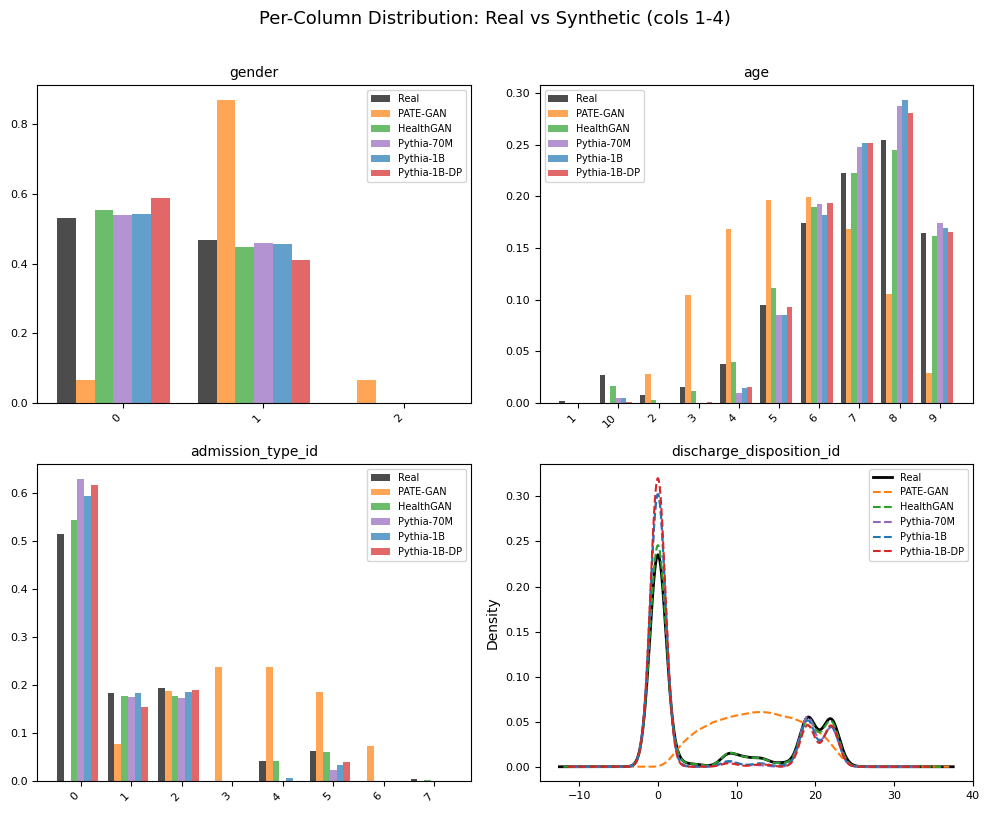
\includegraphics[width=0.95\textwidth]{images/results/marginals_0}
\caption{Per-column marginal distributions, real versus all five
generators (block 1 of 5).}
\label{app:fig:marg0}
\end{figure}

\begin{figure}[H]
\centering
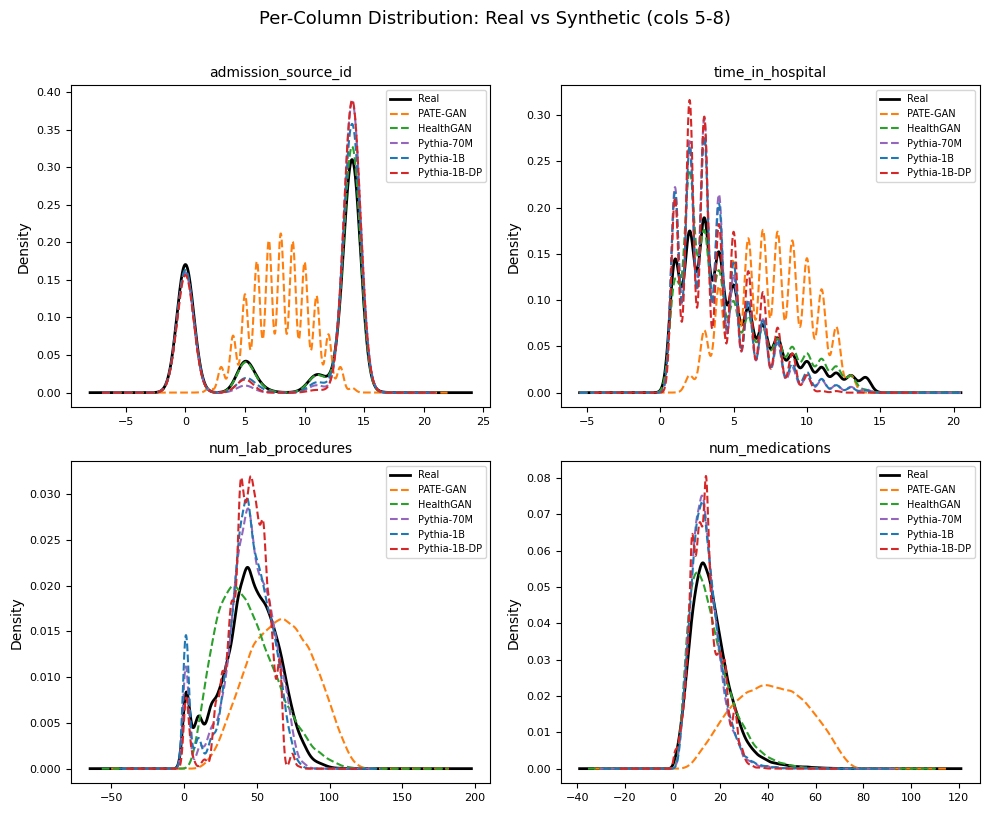
\includegraphics[width=0.95\textwidth]{images/results/marginals_1}
\caption{Per-column marginal distributions, real versus all five
generators (block 2 of 5).}
\label{app:fig:marg1}
\end{figure}

\begin{figure}[H]
\centering
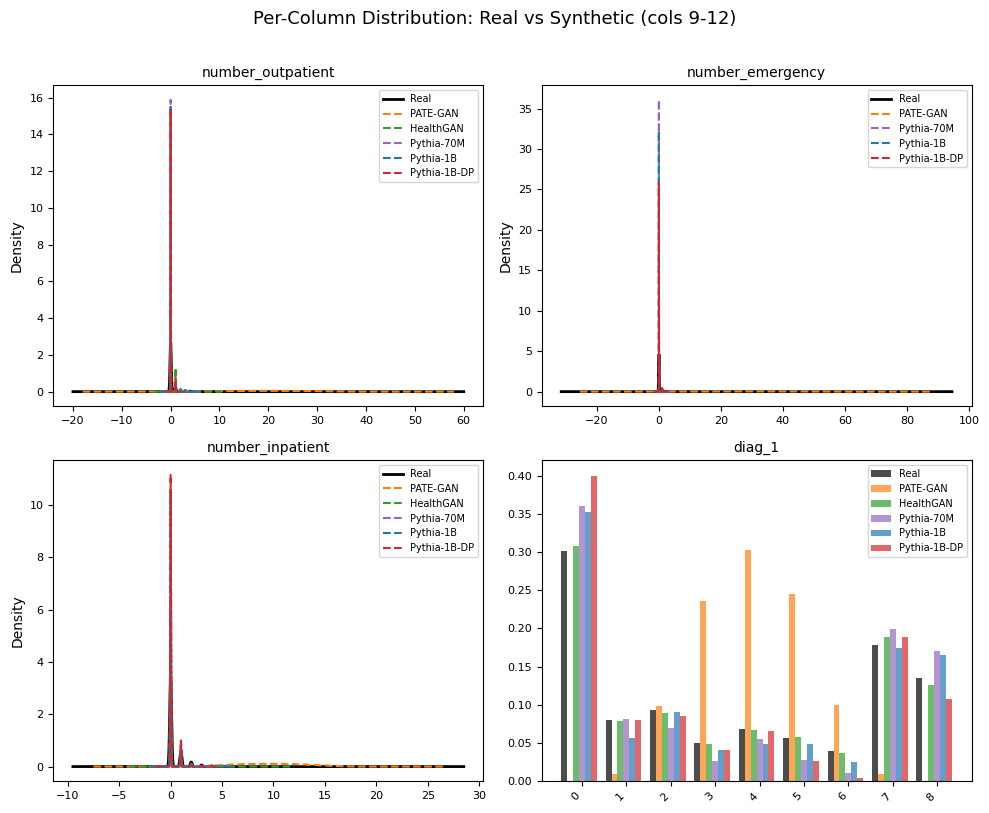
\includegraphics[width=0.95\textwidth]{images/results/marginals_2}
\caption{Per-column marginal distributions, real versus all five
generators (block 3 of 5).}
\label{app:fig:marg2}
\end{figure}

\begin{figure}[H]
\centering
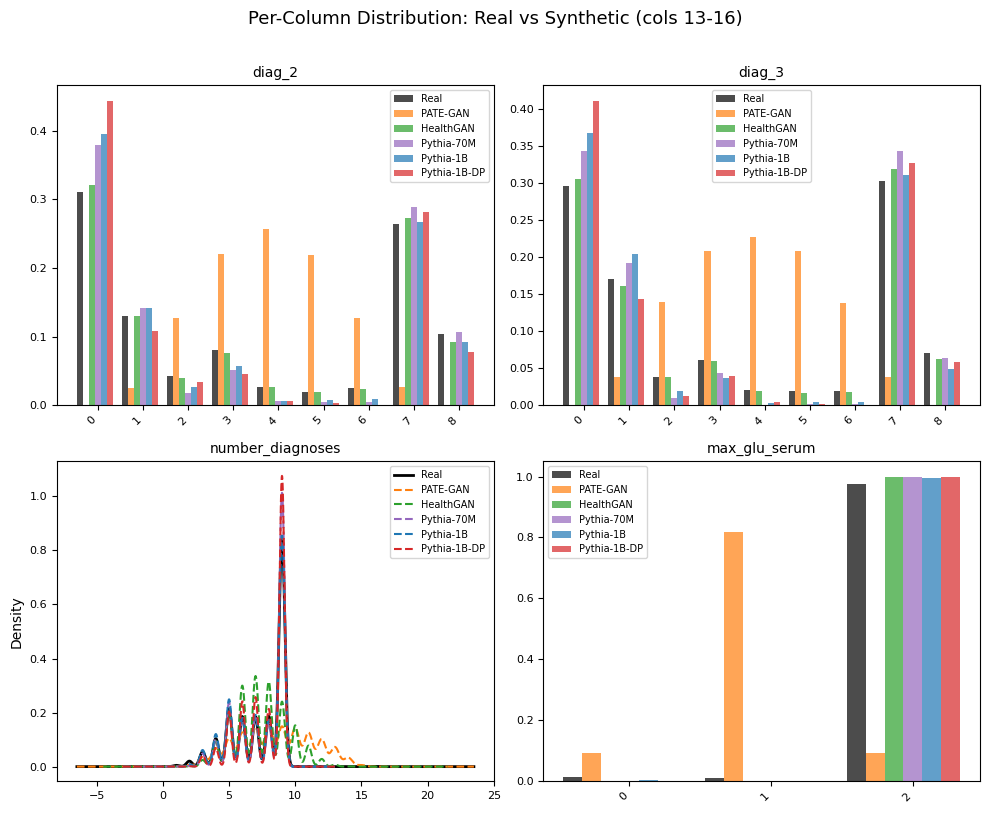
\includegraphics[width=0.95\textwidth]{images/results/marginals_3}
\caption{Per-column marginal distributions, real versus all five
generators (block 4 of 5).}
\label{app:fig:marg3}
\end{figure}

\begin{figure}[H]
\centering
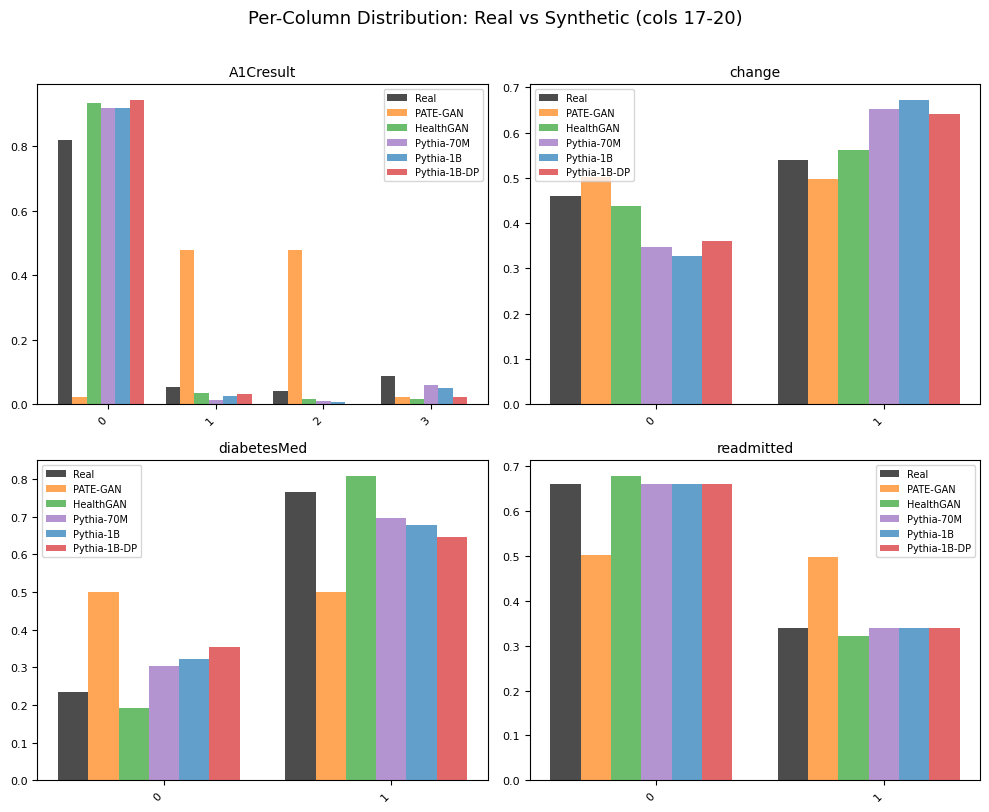
\includegraphics[width=0.95\textwidth]{images/results/marginals_4}
\caption{Per-column marginal distributions, real versus all five
generators (block 5 of 5).}
\label{app:fig:marg4}
\end{figure}

% --------------------------------------------------------------

\chapter{Per-Generator Utility Diagnostics}
\label{app:utility-diag}

The main text reports the class-balance, train--test, correlation-difference,
and survival diagnostics of Section~\ref{sec:results:rq2:utility} in
compressed form. This appendix provides the supporting tables and the full
per-generator visual diagnostics.

\section{Class-Balance and Train--Test Diagnostics}
\label{app:class-balance}

Figure~\ref{app:fig:class-balance} and Table~\ref{app:tab:class-balance}
show the positive-class prevalence of the binary readmission target in the
real and synthetic train/test splits. Table~\ref{app:tab:train-test-auc}
then reports the full AUC-ROC matrix for the TRTR, TSTR, TRTS, and TSTS
regimes.

\begin{figure}[H]
\centering
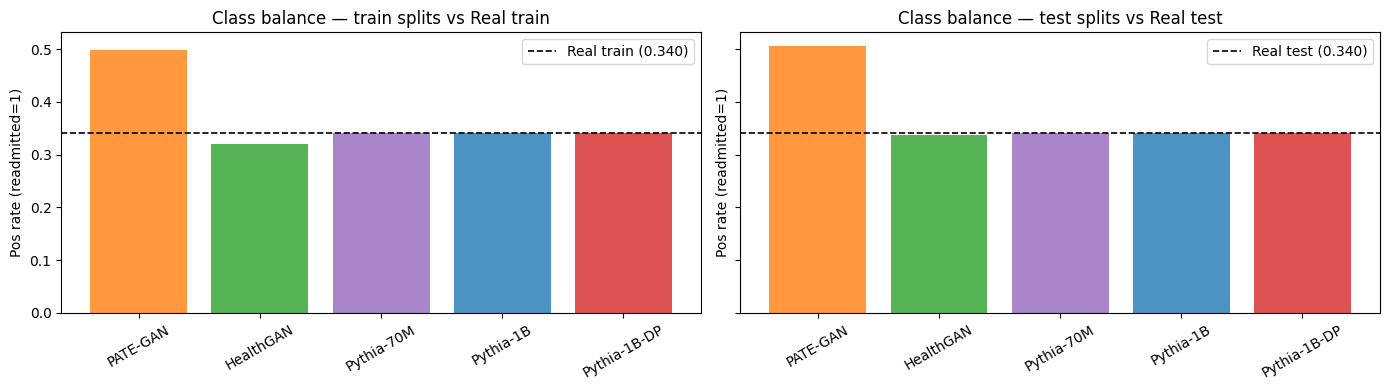
\includegraphics[width=\textwidth]{images/results/class_balance}
\caption{Class balance of the binary readmission target in real and
synthetic train/test splits. The dashed line marks the corresponding
real-split prevalence.}
\label{app:fig:class-balance}
\end{figure}

\begin{table}[H]
\centering
\small
\caption{Readmission class balance by source and split. $\Delta$ is computed
against the matching real split.}
\label{app:tab:class-balance}
\begin{tabular}{llrrrrr}
\toprule
Source & Split & $N$ & Pos (1) & Neg (0) & Pos rate & $\Delta$ vs Real \\
\midrule
Real        & train & 57{,}214 & 19{,}464 & 37{,}750 & 0.340 & $+0.000$ \\
Real        & test  & 14{,}304 & 4{,}866  & 9{,}438  & 0.340 & $+0.000$ \\
PATE-GAN    & train & 57{,}214 & 28{,}500 & 28{,}714 & 0.498 & $+0.158$ \\
HealthGAN   & train & 57{,}214 & 18{,}345 & 38{,}869 & 0.321 & $-0.020$ \\
Pythia-70M  & train & 57{,}214 & 19{,}464 & 37{,}750 & 0.340 & $+0.000$ \\
Pythia-1B   & train & 57{,}214 & 19{,}464 & 37{,}750 & 0.340 & $+0.000$ \\
Pythia-1B-DP & train & 57{,}214 & 19{,}464 & 37{,}750 & 0.340 & $+0.000$ \\
PATE-GAN    & test  & 14{,}304 & 7{,}245  & 7{,}059  & 0.507 & $+0.166$ \\
HealthGAN   & test  & 14{,}304 & 4{,}813  & 9{,}491  & 0.336 & $-0.004$ \\
Pythia-70M  & test  & 14{,}304 & 4{,}866  & 9{,}438  & 0.340 & $+0.000$ \\
Pythia-1B   & test  & 14{,}304 & 4{,}866  & 9{,}438  & 0.340 & $+0.000$ \\
Pythia-1B-DP & test  & 14{,}304 & 4{,}866  & 9{,}438  & 0.340 & $+0.000$ \\
\bottomrule
\end{tabular}
\end{table}

\begin{table}[H]
\centering
\scriptsize
\caption{AUC-ROC by train--test regime. TSTR is the headline downstream
utility regime; TRTS checks synthetic test realism, and TSTS checks internal
synthetic consistency.}
\label{app:tab:train-test-auc}
\begin{tabular}{llcccc}
\toprule
Synthetic Source & Classifier & TRTR & TSTR & TRTS & TSTS \\
\midrule
HealthGAN & Gradient Boosting & 0.7008 & 0.6312 & 0.6531 & 0.6191 \\
HealthGAN & Logistic Regression & 0.6670 & 0.6130 & 0.6499 & 0.6103 \\
HealthGAN & Random Forest & 0.6790 & 0.6153 & 0.6366 & 0.6021 \\
\midrule
PATE-GAN & Gradient Boosting & 0.7008 & 0.5108 & 0.4601 & 0.5323 \\
PATE-GAN & Logistic Regression & 0.6670 & 0.5079 & 0.5082 & 0.5432 \\
PATE-GAN & Random Forest & 0.6790 & 0.5018 & 0.5040 & 0.5302 \\
\midrule
Pythia-1B & Gradient Boosting & 0.7008 & 0.6818 & 0.6980 & 0.7119 \\
Pythia-1B & Logistic Regression & 0.6670 & 0.6613 & 0.6822 & 0.6969 \\
Pythia-1B & Random Forest & 0.6790 & 0.6682 & 0.6635 & 0.8343 \\
\midrule
Pythia-1B-DP & Gradient Boosting & 0.7008 & 0.5827 & 0.5338 & 0.5403 \\
Pythia-1B-DP & Logistic Regression & 0.6670 & 0.5868 & 0.5013 & 0.5236 \\
Pythia-1B-DP & Random Forest & 0.6790 & 0.5823 & 0.5353 & 0.6213 \\
\midrule
Pythia-70M & Gradient Boosting & 0.7008 & 0.6634 & 0.5939 & 0.5920 \\
Pythia-70M & Logistic Regression & 0.6670 & 0.6573 & 0.5882 & 0.5893 \\
Pythia-70M & Random Forest & 0.6790 & 0.6588 & 0.5678 & 0.5720 \\
\bottomrule
\end{tabular}
\end{table}

\section{Correlation-Difference Heatmaps}
\label{app:corrheat}

Figure~\ref{app:fig:corrheat} gives the correlation-difference heatmaps
(real minus synthetic correlation matrix) for all five generators,
extending the contrast of Figure~\ref{fig:rq2:corrheat}. Saturated cells
denote large residual correlation; pale cells denote faithful
reproduction of the pairwise dependency structure.

\begin{figure}[H]
\centering
\begin{subfigure}{0.48\textwidth}\centering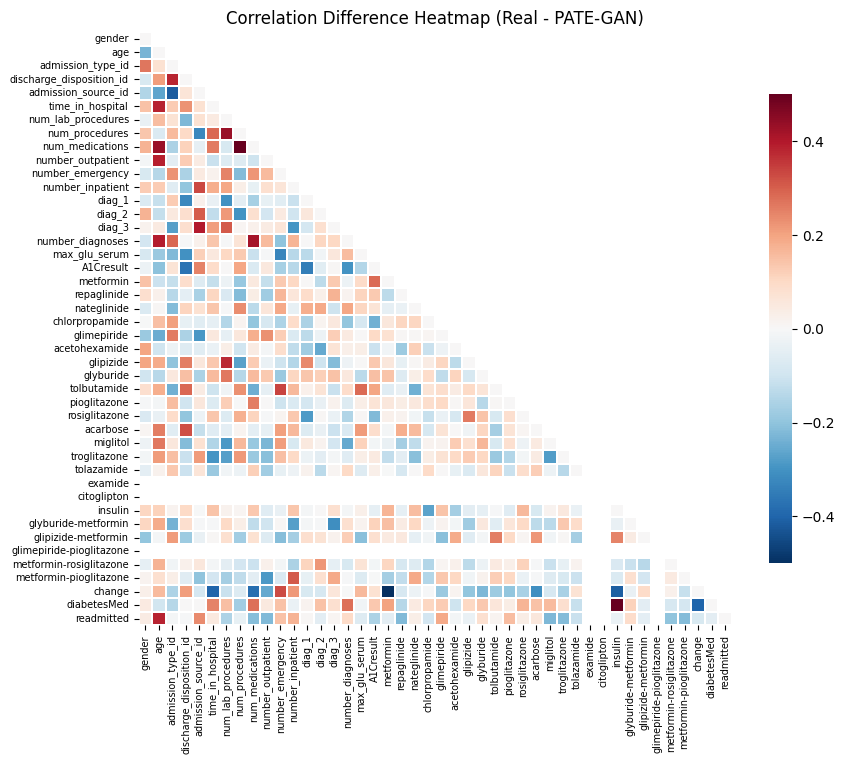
\includegraphics[width=\textwidth]{images/results/corrheat_0}\caption{PATE-GAN}\end{subfigure}\hfill
\begin{subfigure}{0.48\textwidth}\centering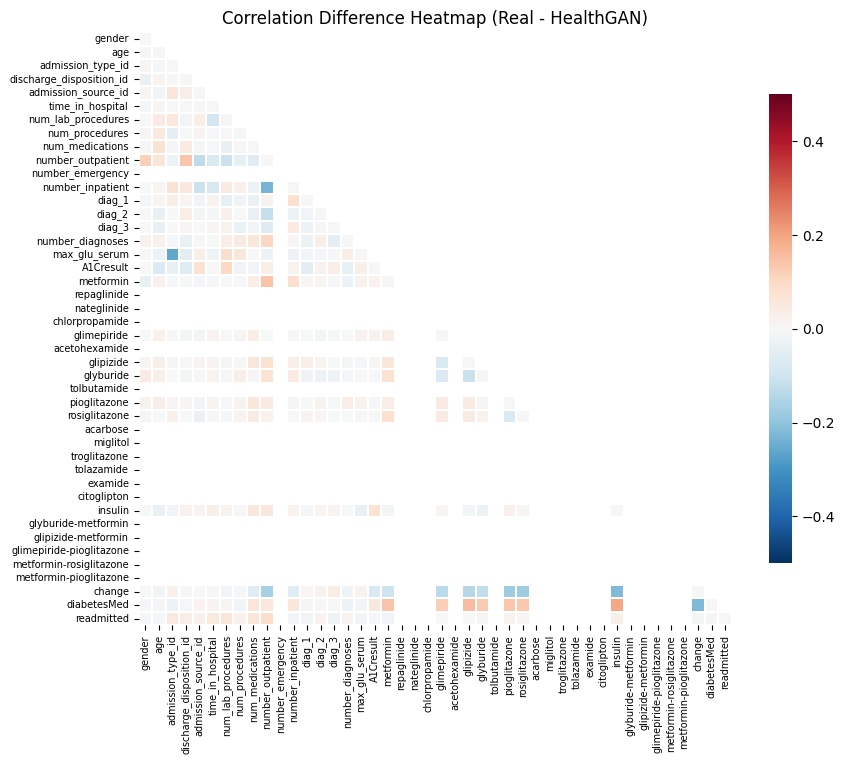
\includegraphics[width=\textwidth]{images/results/corrheat_1}\caption{HealthGAN}\end{subfigure}

\vspace{1ex}
\begin{subfigure}{0.48\textwidth}\centering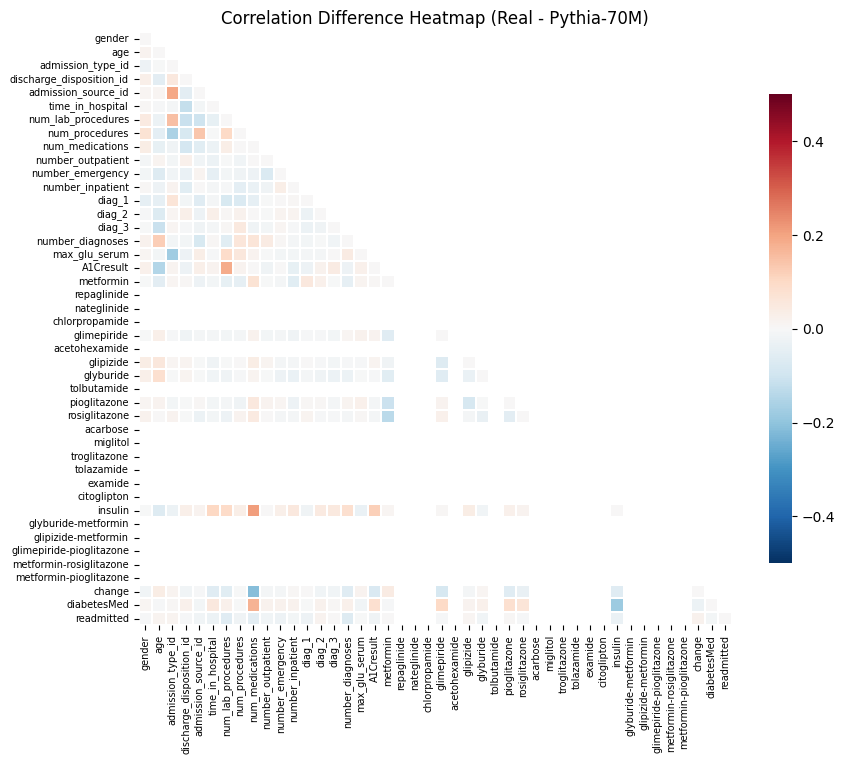
\includegraphics[width=\textwidth]{images/results/corrheat_2}\caption{Pythia-70M}\end{subfigure}\hfill
\begin{subfigure}{0.48\textwidth}\centering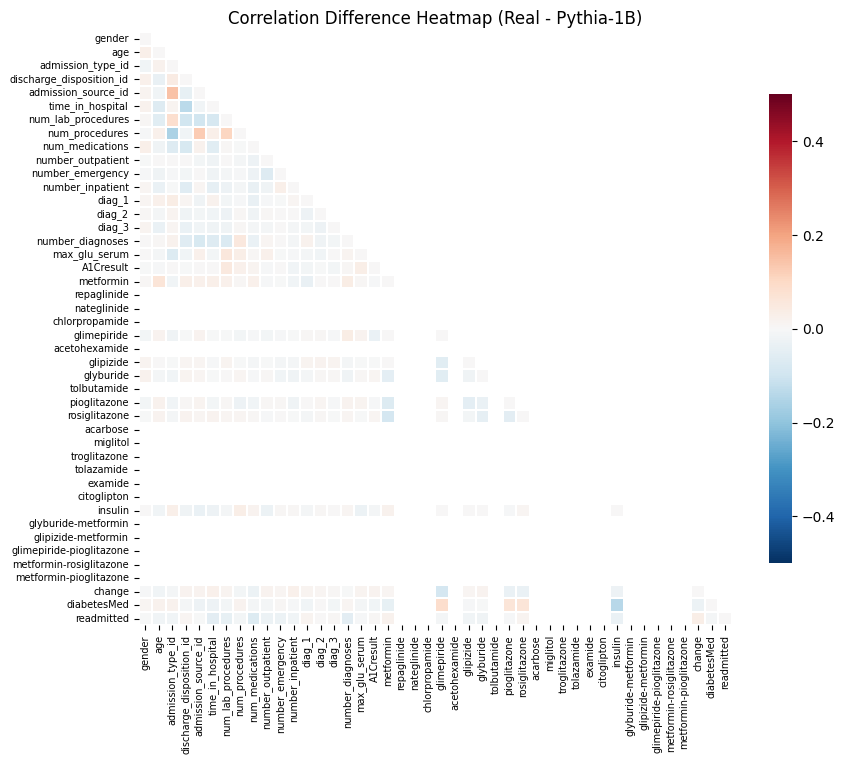
\includegraphics[width=\textwidth]{images/results/corrheat_3}\caption{Pythia-1B}\end{subfigure}

\vspace{1ex}
\begin{subfigure}{0.48\textwidth}\centering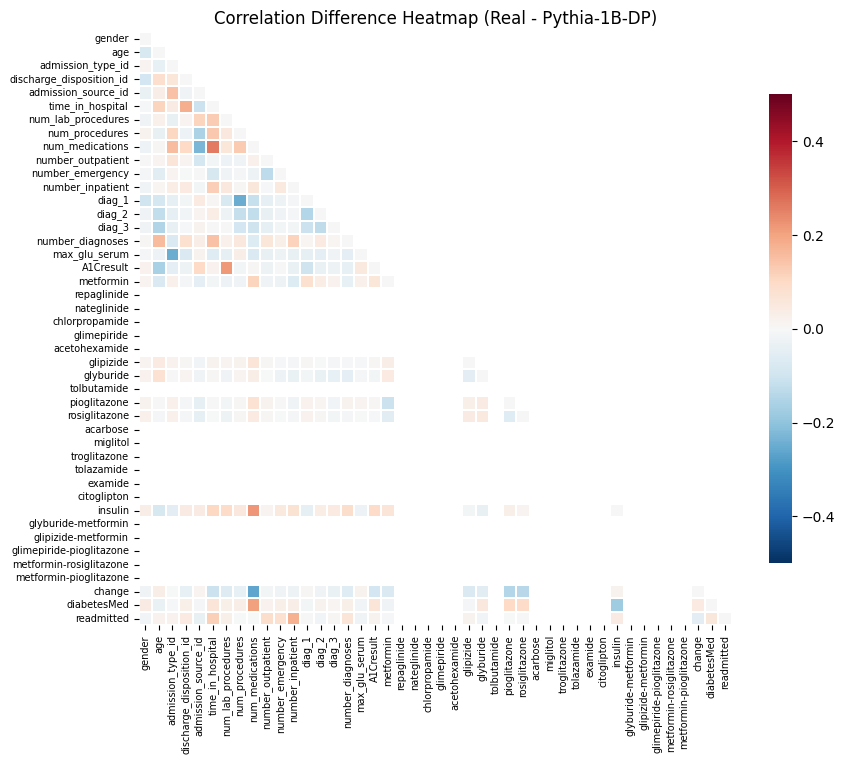
\includegraphics[width=\textwidth]{images/results/corrheat_4}\caption{Pythia-1B-DP}\end{subfigure}
\caption{Correlation-difference heatmaps (real minus synthetic) for all
five generators.}
\label{app:fig:corrheat}
\end{figure}

\section{Cox Proportional-Hazards Estimates}
\label{app:cox}

Figure~\ref{app:fig:cox} gives the Cox hazard-ratio plots (real in black
versus synthetic in colour, with shaded rows marking non-overlapping
confidence intervals) for all five generators, extending the contrast of
Figure~\ref{fig:rq2:cox}. The per-generator confidence-interval overlap
counts are reported in Table~\ref{tab:rq2:cox}.

\begin{figure}[H]
\centering
\begin{subfigure}{0.48\textwidth}\centering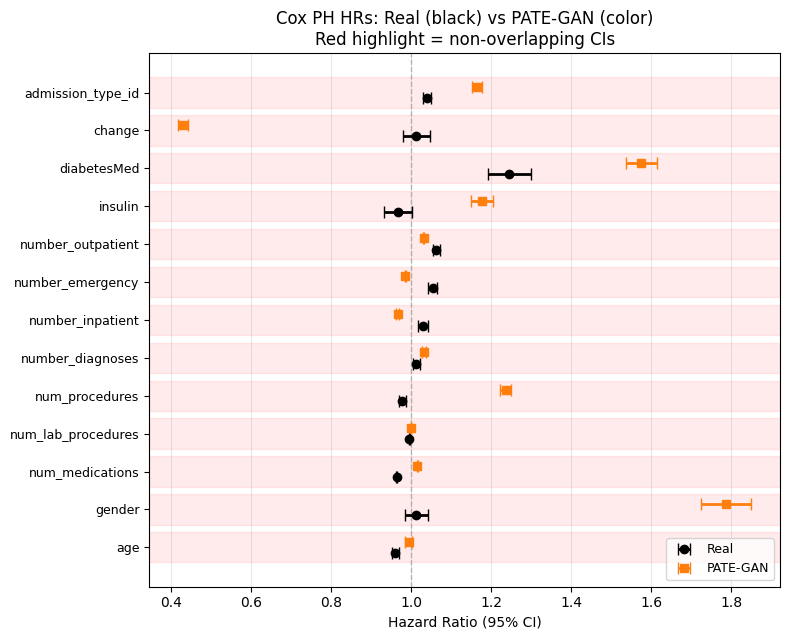
\includegraphics[width=\textwidth]{images/results/cox_0}\caption{PATE-GAN (0/13)}\end{subfigure}\hfill
\begin{subfigure}{0.48\textwidth}\centering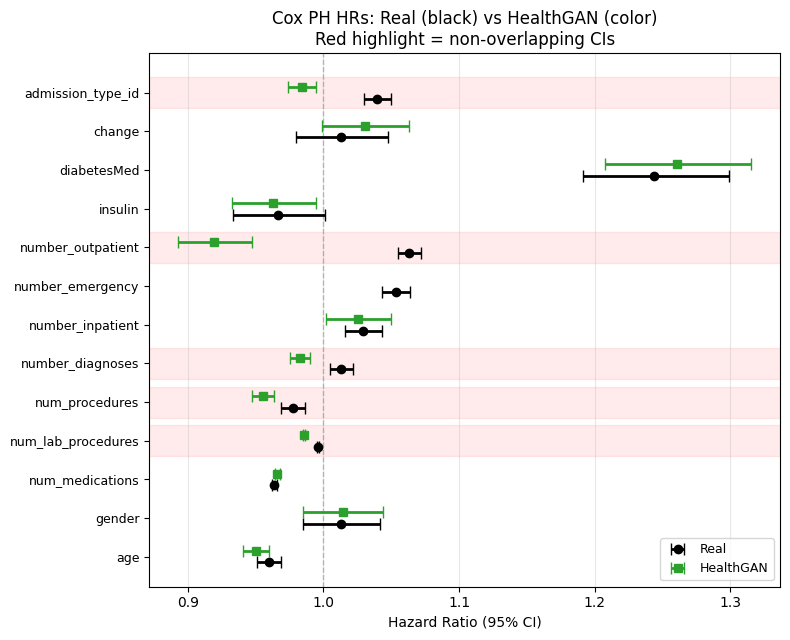
\includegraphics[width=\textwidth]{images/results/cox_1}\caption{HealthGAN (7/12)}\end{subfigure}

\vspace{1ex}
\begin{subfigure}{0.48\textwidth}\centering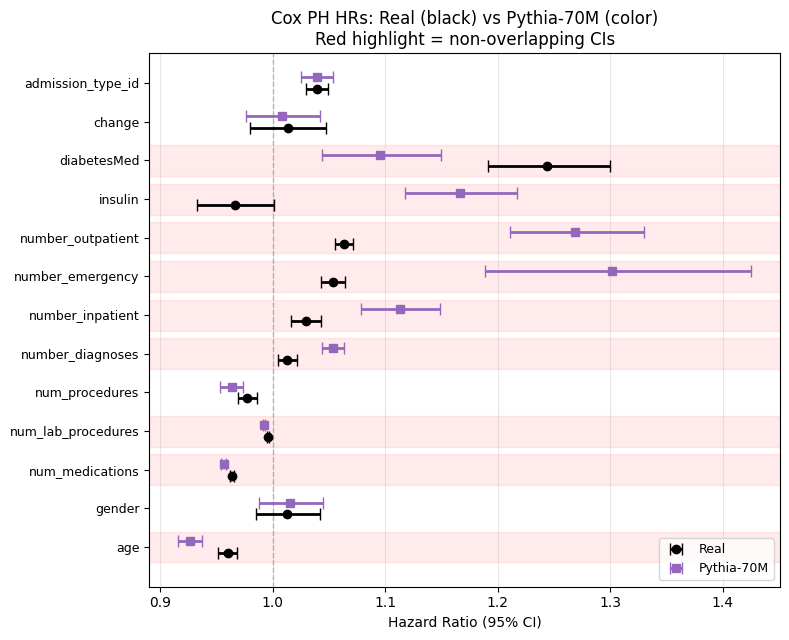
\includegraphics[width=\textwidth]{images/results/cox_2}\caption{Pythia-70M (4/13)}\end{subfigure}\hfill
\begin{subfigure}{0.48\textwidth}\centering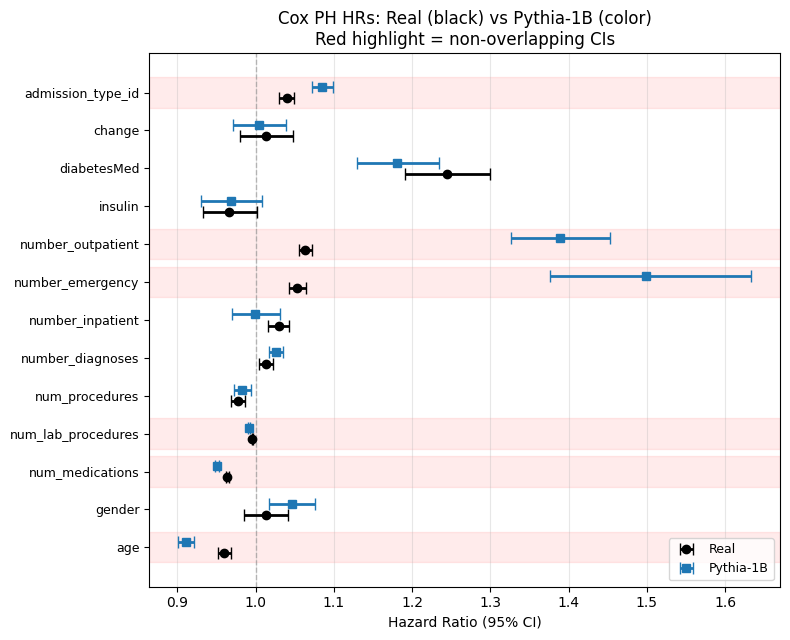
\includegraphics[width=\textwidth]{images/results/cox_3}\caption{Pythia-1B (7/13)}\end{subfigure}

\vspace{1ex}
\begin{subfigure}{0.48\textwidth}\centering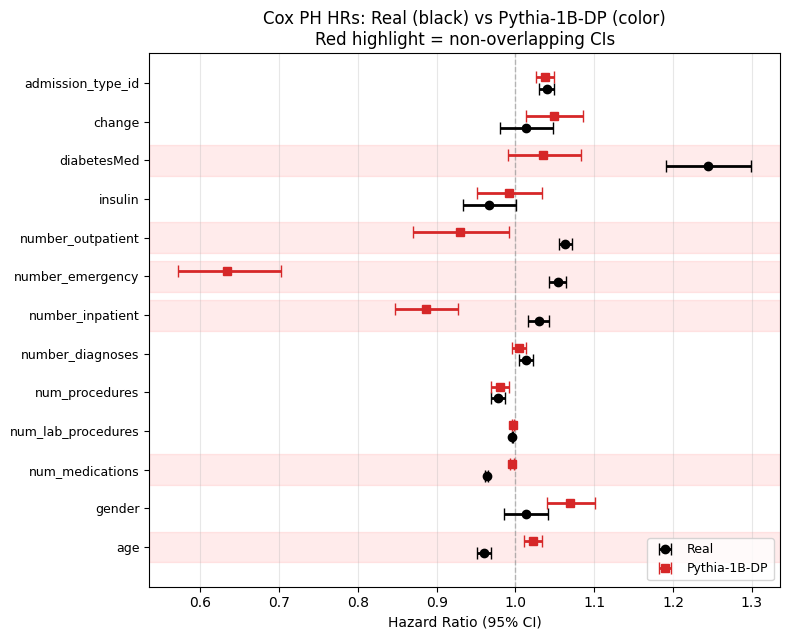
\includegraphics[width=\textwidth]{images/results/cox_4}\caption{Pythia-1B-DP (7/13)}\end{subfigure}
\caption{Cox hazard-ratio estimates with $95\%$ confidence intervals for
all five generators; subcaptions report the overlap count with the real
intervals.}
\label{app:fig:cox}
\end{figure}

% --------------------------------------------------------------

\chapter{Per-Attribute Privacy Risk}
\label{app:privacy-detail}

% TODO: Detailed per-attribute breakdown of attribute-inference advantage
% (§4.2). The main text reports max advantage; here, list every attribute
% × generator cell with the actual value.

% --------------------------------------------------------------

\chapter{Reproducibility}
\label{app:reproducibility}

\section{Repository Layout}
% TODO: tree-style listing of the project showing
%   thesis/, healthgan/, Pategan/, pythia/, and the shared data/ directory.

\section{Run Commands}
% TODO: shell snippets for each pipeline:

% \begin{verbatim}
% # 1. Preprocess
% python -m thesis.feature_engineering ...
%
% # 2. Generate HealthGAN synthetic data
% python healthgan/generators/sdv_converter.py ... encode
% python healthgan/generators/wgan_for_mac.py 5 64
% python healthgan/generators/sdv_converter.py ... decode samples_99999_5_64.npy
%
% # 3. Generate PATE-GAN synthetic data
% python Pategan/generate_pategan_synthetic.py --epsilon 5.0 --splits train test
%
% # 4. Generate Pythia synthetic data (non-DP)
% python pythia/generate_pythia_synthetic.py --splits train test
%
% # 5. Generate Pythia synthetic data (DP)
% python pythia/generate_pythia_synthetic_dp.py --dp \
%        --target-epsilon 5.0 --target-delta 1e-5
%
% # 6. Evaluate
% jupyter execute thesis/data_analysis.ipynb
% \end{verbatim}

\section{Run Metadata Excerpts}
% TODO: include excerpts from
%   thesis/data/pythia/run_metadata.json
%   thesis/data/pythia/run_metadata_dp.json
% showing achieved_epsilon, training duration, hardware.

\section{Computational Environment}
% TODO: Python version, key library versions (torch, opacus, transformers,
% peft, tensorflow, scikit-learn, lifelines), GPU model and memory, OS.
% Wall-clock time per generator.

% --------------------------------------------------------------

\chapter{HealthGAN Variant Comparison}
\label{app:hg-variants}

This appendix provides the visual diagnostics supporting the sample-selection
analysis of Section~\ref{sec:methods:healthgan:variants}, which compares the
three retained HealthGAN draws (indexed $0$, $3$, and $6$) and carries draw
$0$ forward as representative. The headline fidelity figures --- mean
Kolmogorov--Smirnov statistic and mean correlation difference per draw ---
are given in Table~\ref{tab:hg-variants}; the figures below show that the
three draws are visually indistinguishable from one another and from the
real data on every diagnostic, supporting the use of draw $0$ as a representative sample.

The diagnostics in this appendix were generated in the HealthGAN-only
fidelity analysis of \texttt{data\_analysis.ipynb}, using the real training
partition and the three retained decoded HealthGAN draws labelled
HealthGAN-0, HealthGAN-3, and HealthGAN-6 in that analysis.

\section{Per-Column Marginal Distributions}
\label{app:hg-variants:marginals}

\begin{figure}[H]
\centering
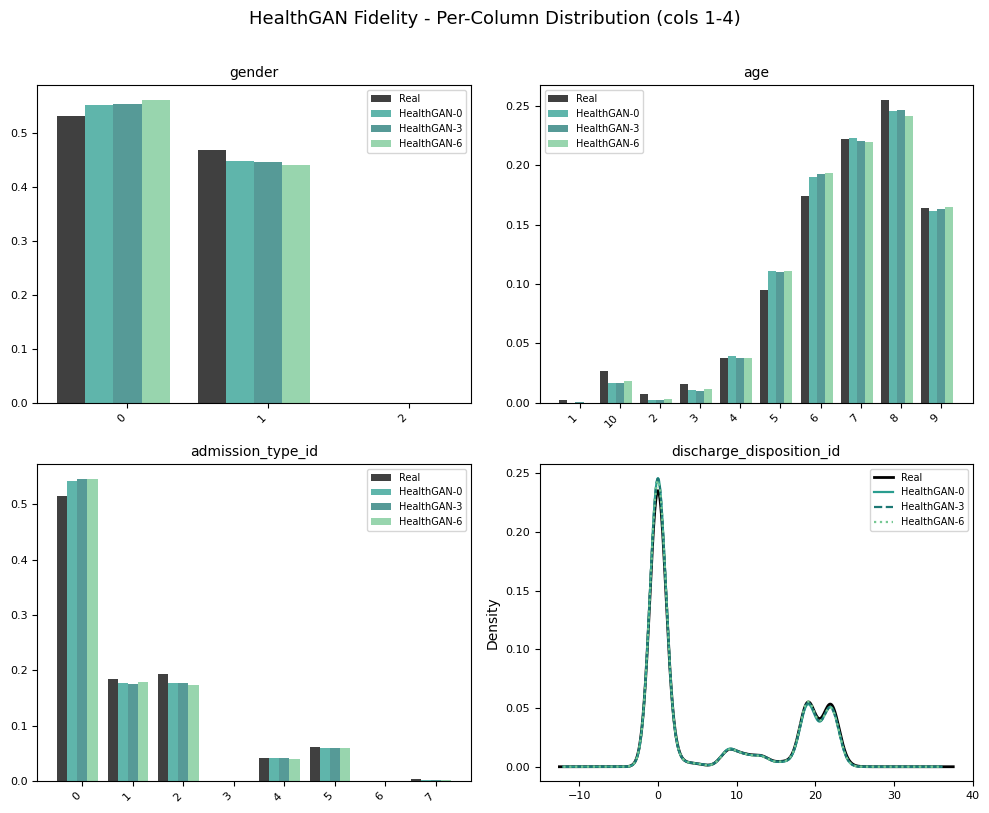
\includegraphics[width=0.92\textwidth]{images/results/hg_marginals_0}
\caption{Per-column marginal distributions, real versus the three HealthGAN
draws (block 1 of 5).}
\label{app:fig:hgmarg0}
\end{figure}

\begin{figure}[H]
\centering
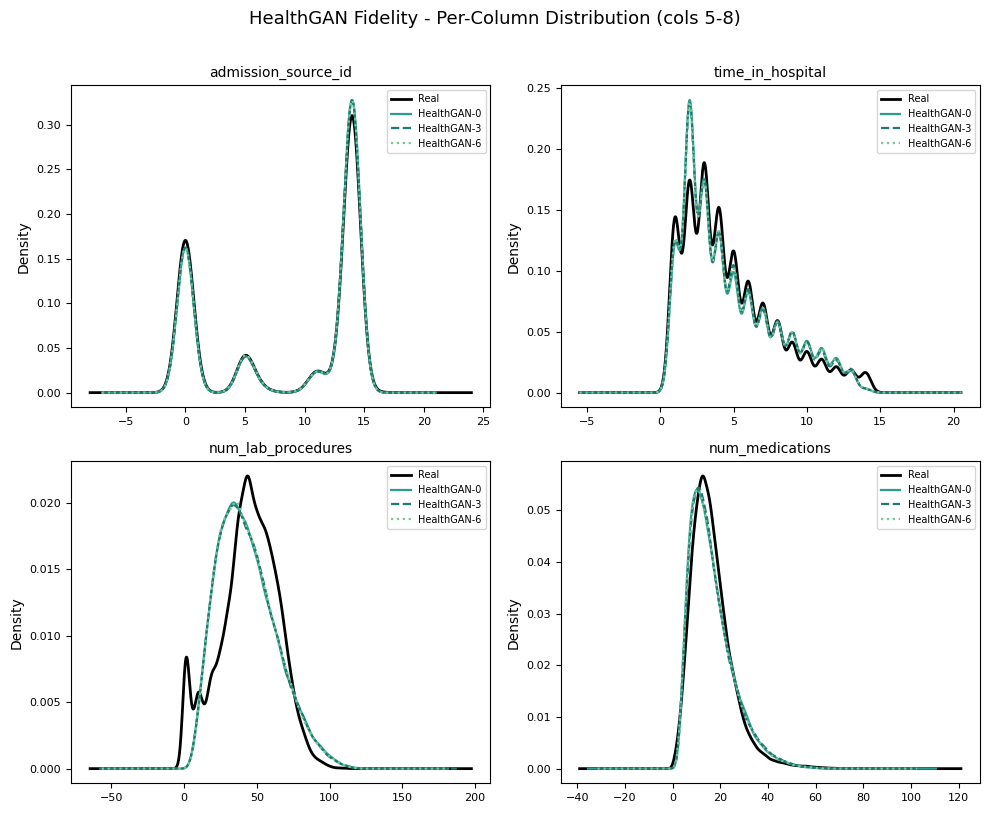
\includegraphics[width=0.92\textwidth]{images/results/hg_marginals_1}
\caption{Per-column marginal distributions, real versus the three HealthGAN
draws (block 2 of 5).}
\label{app:fig:hgmarg1}
\end{figure}

\begin{figure}[H]
\centering
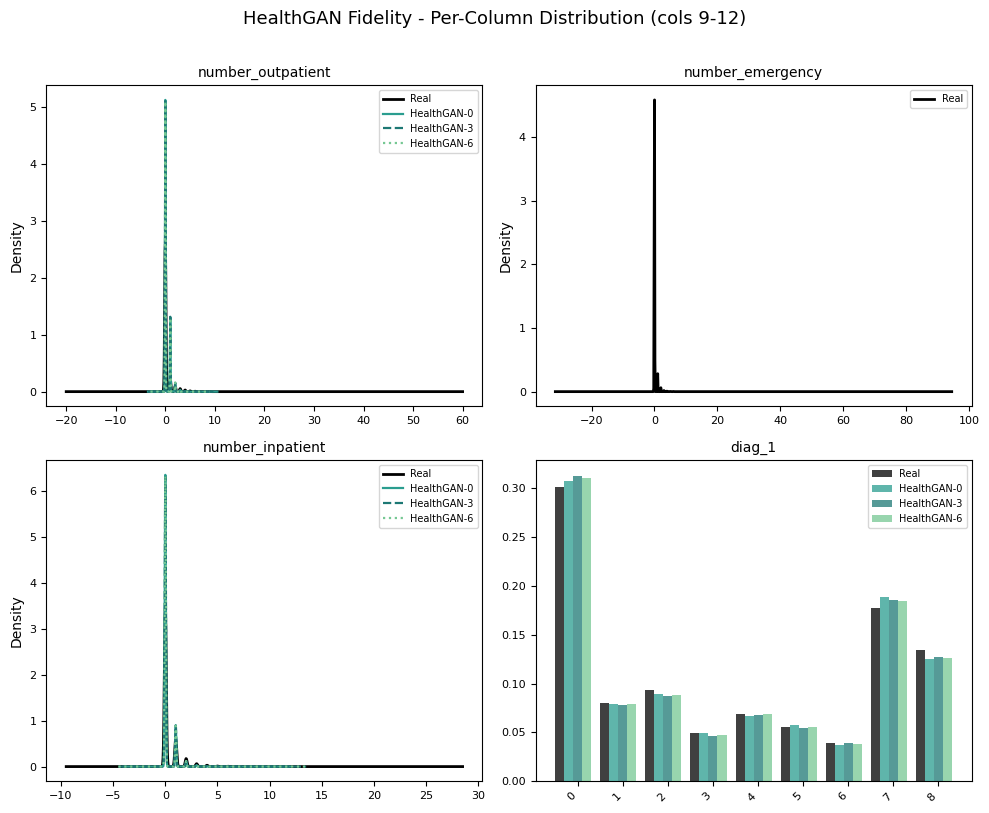
\includegraphics[width=0.92\textwidth]{images/results/hg_marginals_2}
\caption{Per-column marginal distributions, real versus the three HealthGAN
draws (block 3 of 5).}
\label{app:fig:hgmarg2}
\end{figure}

\begin{figure}[H]
\centering
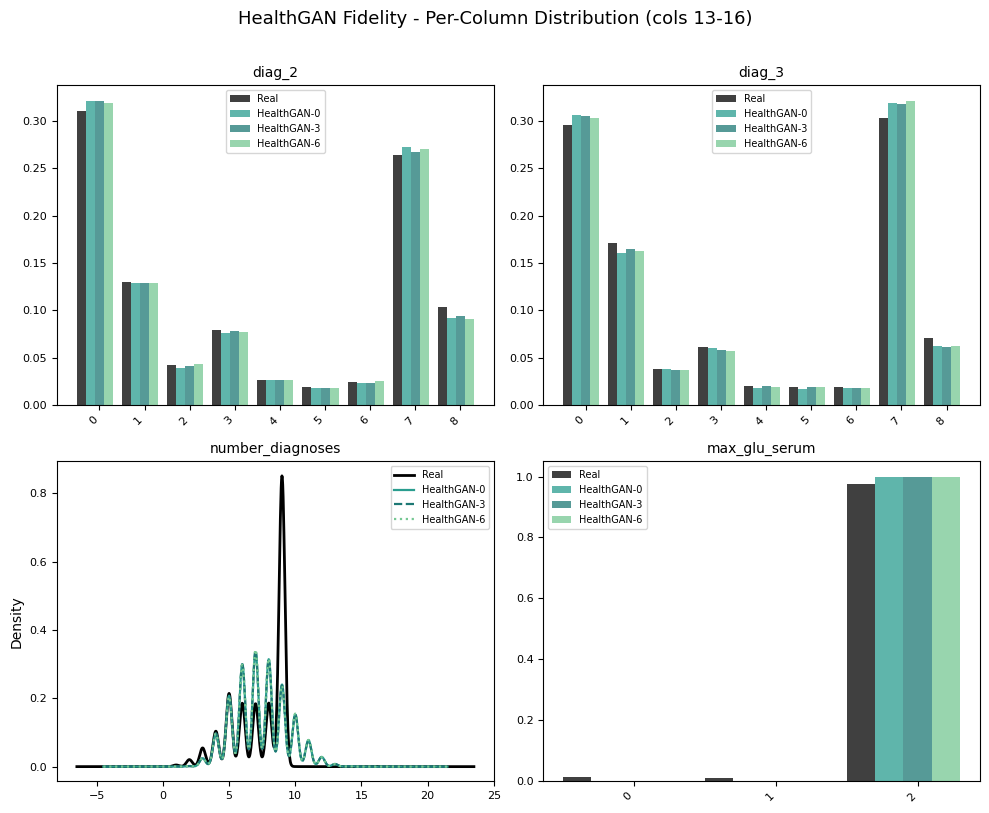
\includegraphics[width=0.92\textwidth]{images/results/hg_marginals_3}
\caption{Per-column marginal distributions, real versus the three HealthGAN
draws (block 4 of 5).}
\label{app:fig:hgmarg3}
\end{figure}

\begin{figure}[H]
\centering
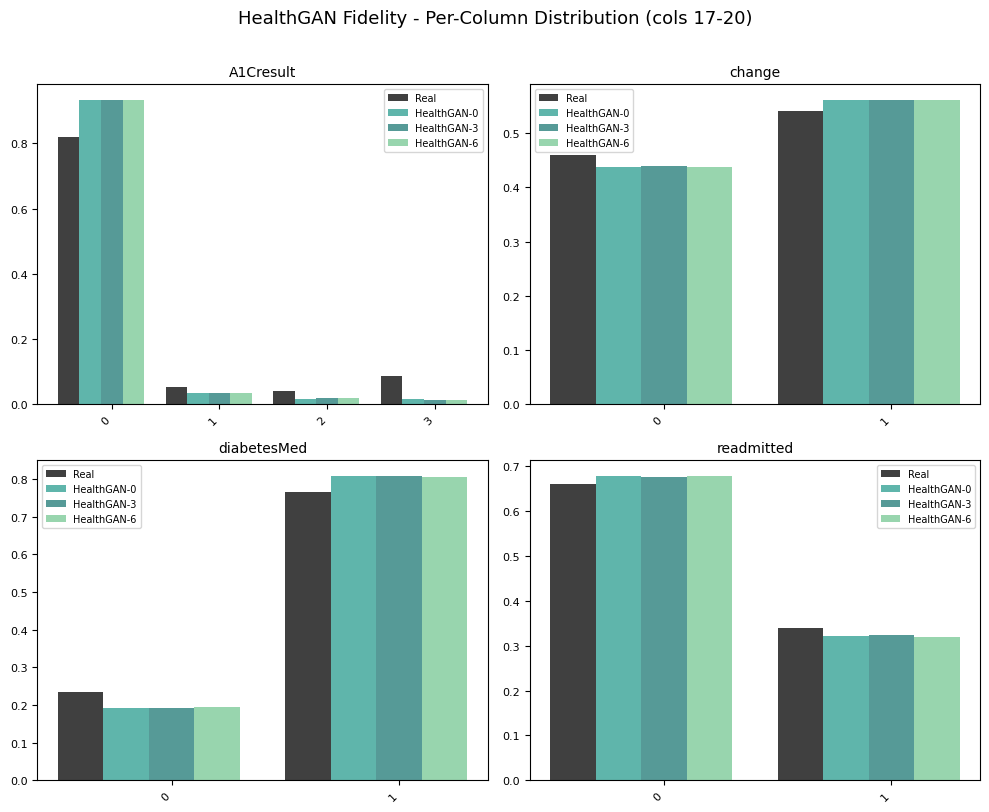
\includegraphics[width=0.92\textwidth]{images/results/hg_marginals_4}
\caption{Per-column marginal distributions, real versus the three HealthGAN
draws (block 5 of 5).}
\label{app:fig:hgmarg4}
\end{figure}

\section{Descriptive Statistics}
\label{app:hg-variants:desc}

\begin{table}[H]
\centering
\small
\caption{Selected per-column means for the real training partition and the
three retained HealthGAN draws.}
\label{app:tab:hg-means}
\begin{tabular}{lrrrr}
\toprule
Column & Real & HG-0 & HG-3 & HG-6 \\
\midrule
gender & 0.468 & 0.448 & 0.446 & 0.440 \\
age & 7.074 & 7.030 & 7.040 & 7.037 \\
admission\_type\_id & 1.082 & 1.011 & 1.004 & 0.999 \\
discharge\_disposition\_id & 6.875 & 6.513 & 6.540 & 6.595 \\
admission\_source\_id & 8.876 & 9.155 & 9.167 & 9.157 \\
time\_in\_hospital & 4.763 & 4.740 & 4.728 & 4.730 \\
num\_lab\_procedures & 44.181 & 43.550 & 43.552 & 43.541 \\
num\_medications & 16.407 & 16.461 & 16.528 & 16.392 \\
number\_outpatient & 0.305 & 0.263 & 0.265 & 0.266 \\
number\_emergency & 0.124 & 0.000 & 0.000 & 0.000 \\
number\_inpatient & 0.320 & 0.174 & 0.173 & 0.173 \\
diag\_1 & 3.523 & 3.504 & 3.494 & 3.487 \\
diag\_2 & 3.480 & 3.420 & 3.413 & 3.418 \\
diag\_3 & 3.415 & 3.417 & 3.408 & 3.440 \\
number\_diagnoses & 7.346 & 7.364 & 7.359 & 7.364 \\
max\_glu\_serum & 1.961 & 2.000 & 2.000 & 2.000 \\
A1Cresult & 0.395 & 0.113 & 0.113 & 0.112 \\
change & 0.540 & 0.562 & 0.561 & 0.562 \\
diabetesMed & 0.766 & 0.809 & 0.808 & 0.805 \\
readmitted & 0.340 & 0.321 & 0.324 & 0.321 \\
\bottomrule
\end{tabular}
\end{table}

\begin{table}[H]
\centering
\small
\caption{Selected per-column standard deviations for the real training
partition and the three retained HealthGAN draws.}
\label{app:tab:hg-std}
\begin{tabular}{lrrrr}
\toprule
Column & Real & HG-0 & HG-3 & HG-6 \\
\midrule
gender & 0.499 & 0.497 & 0.497 & 0.496 \\
age & 1.598 & 1.507 & 1.501 & 1.514 \\
admission\_type\_id & 1.495 & 1.457 & 1.452 & 1.451 \\
discharge\_disposition\_id & 9.186 & 9.033 & 9.044 & 9.066 \\
admission\_source\_id & 6.311 & 6.234 & 6.225 & 6.221 \\
time\_in\_hospital & 3.183 & 3.187 & 3.175 & 3.185 \\
num\_lab\_procedures & 19.964 & 20.144 & 20.051 & 19.963 \\
num\_medications & 8.644 & 9.103 & 9.175 & 9.094 \\
number\_outpatient & 1.127 & 0.539 & 0.539 & 0.541 \\
number\_emergency & 0.650 & 0.000 & 0.000 & 0.000 \\
number\_inpatient & 0.810 & 0.479 & 0.483 & 0.481 \\
diag\_1 & 3.115 & 3.116 & 3.127 & 3.118 \\
diag\_2 & 3.204 & 3.199 & 3.199 & 3.192 \\
diag\_3 & 3.179 & 3.190 & 3.185 & 3.190 \\
number\_diagnoses & 1.972 & 1.996 & 1.996 & 1.992 \\
max\_glu\_serum & 0.255 & 0.010 & 0.004 & 0.010 \\
A1Cresult & 0.916 & 0.472 & 0.470 & 0.470 \\
change & 0.498 & 0.496 & 0.496 & 0.496 \\
diabetesMed & 0.423 & 0.393 & 0.394 & 0.396 \\
readmitted & 0.474 & 0.467 & 0.468 & 0.467 \\
\bottomrule
\end{tabular}
\end{table}

\section{Correlation Structure and Manifold Overlap}
\label{app:hg-variants:corr-pca}

\begin{figure}[H]
\centering
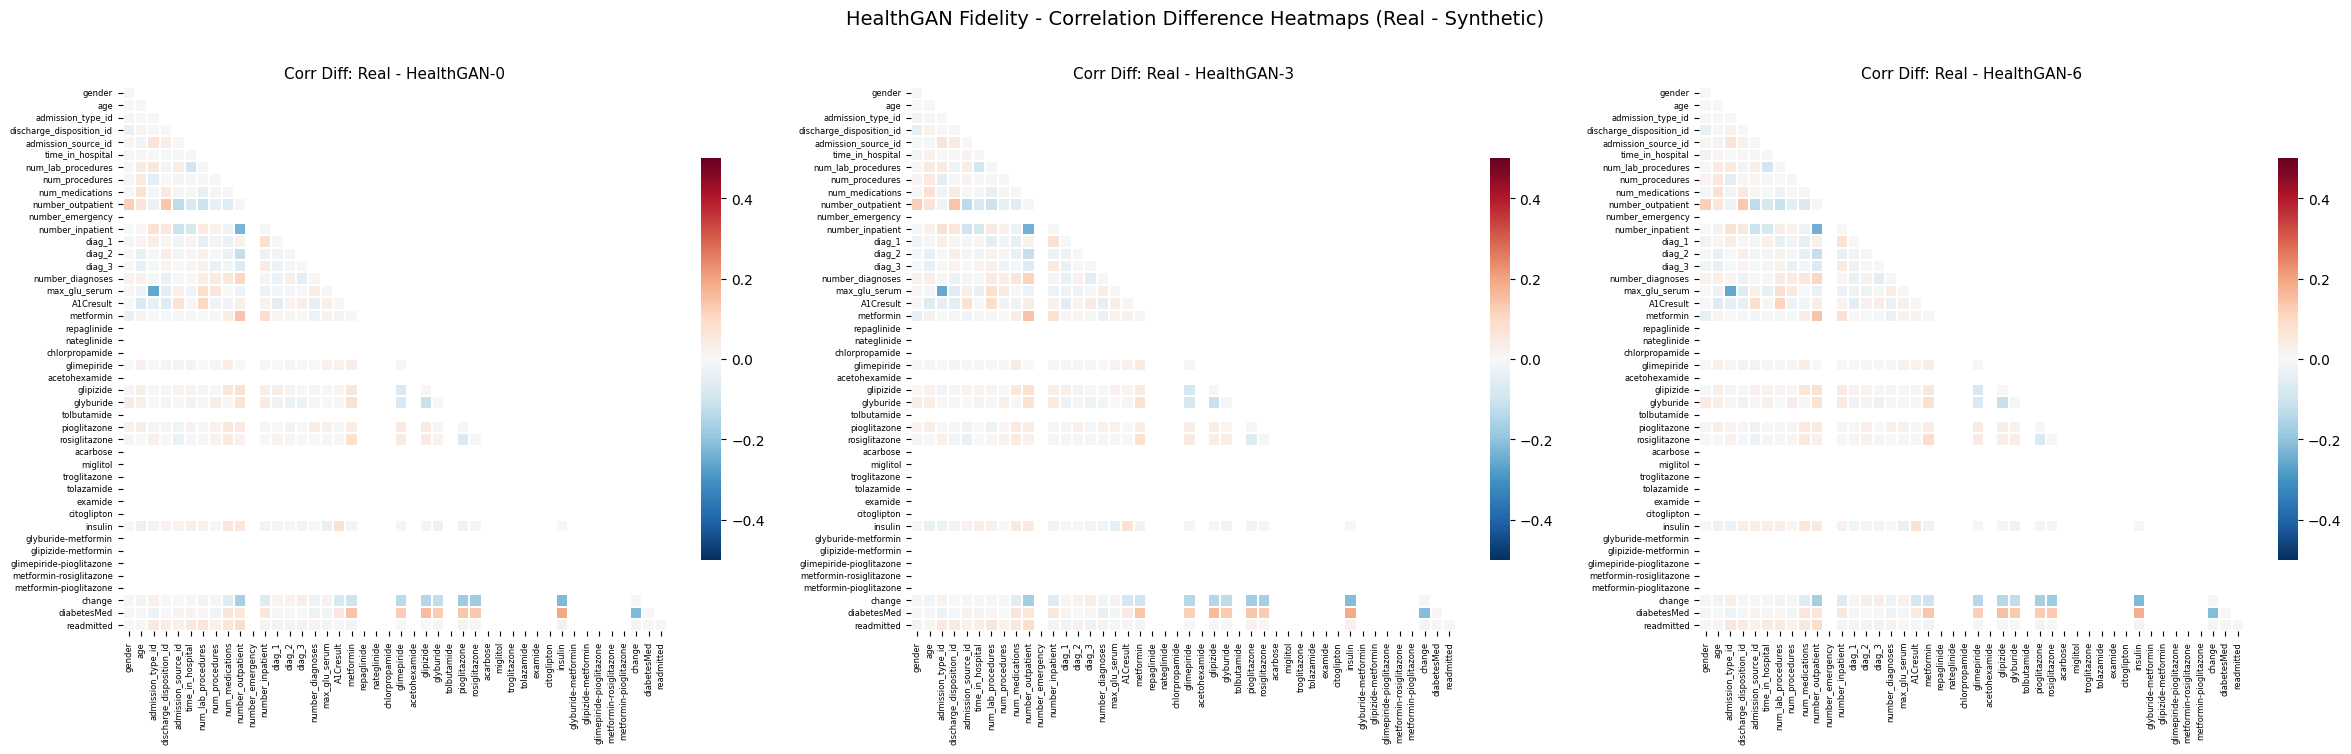
\includegraphics[width=0.92\textwidth]{images/results/hg_corrheat}
\caption{Correlation-difference heatmaps (real minus synthetic) for the
three HealthGAN draws.}
\label{app:fig:hgcorr}
\end{figure}

\begin{figure}[H]
\centering
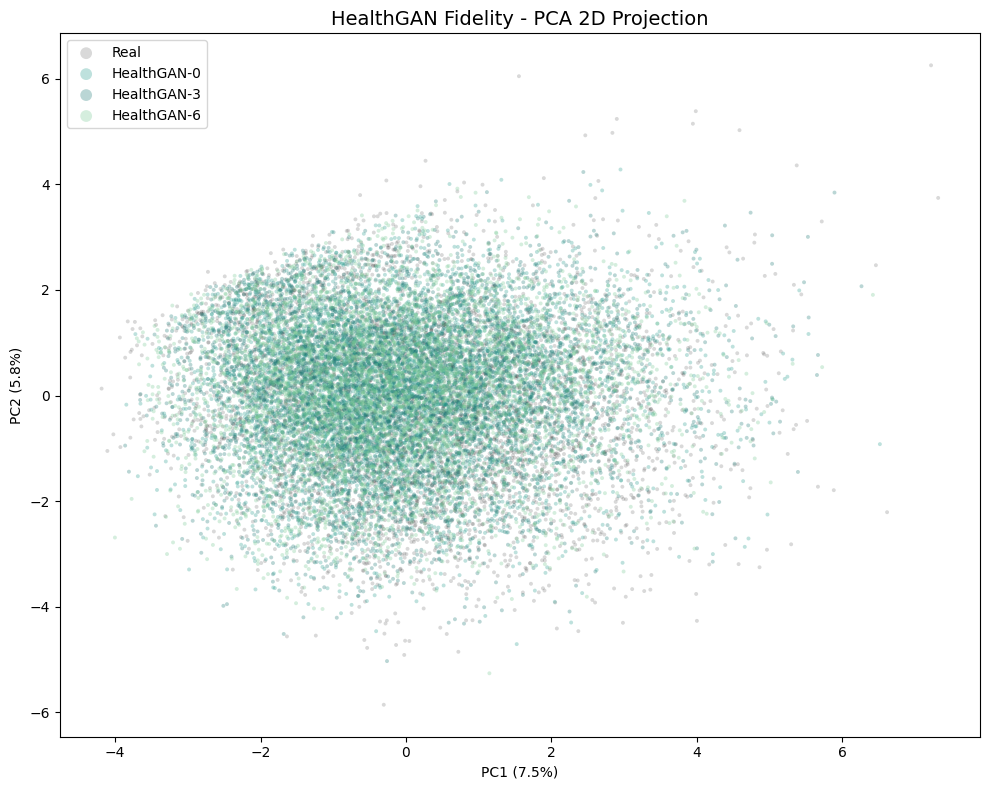
\includegraphics[width=0.7\textwidth]{images/results/hg_pca}
\caption{Two-dimensional PCA projection of the real data and the three
HealthGAN draws; the three draws overlap one another and the real cloud.}
\label{app:fig:hgpca}
\end{figure}


\end{document}
